\documentclass[10pt,a4paper,onecolumn]{article} \usepackage[latin1]{inputenc}
\usepackage{amsmath,enumitem,datetime,xfrac,fix-cm,color,multirow,siunitx}
\usepackage{amsfonts,amssymb,mathtools,stmaryrd,dsfont,tikz,amsthm}
\usepackage[cm]{fullpage}
\definecolor{linkColor}{rgb}{0.5, 0.5, 0.5}
\usepackage[colorlinks, allcolors=linkColor, bookmarks=True]{hyperref}
\usepackage[capitalise]{cleveref}
\usetikzlibrary{positioning,trees}
\usepackage{algorithm,algpseudocode}
\graphicspath{{Figures/}}
\DeclareGraphicsExtensions{.pdf,.png}
\numberwithin{equation}{section}
\newtheorem{definition}{Definition}[section]\newtheorem{theorem}{Theorem}[section]
\newtheorem{lemma}{Lemma}[section]\newtheorem{example}{Example}[section]
\newtheorem{remark}{Remark}[section]
\makeatletter\let\c@definition\c@theorem\let\c@definition\c@theorem\makeatother
\makeatletter\let\c@lemma\c@theorem\let\c@lemma\c@theorem\makeatother
\makeatletter\let\c@example\c@theorem\let\c@example\c@theorem\makeatother
\makeatletter\let\c@remark\c@theorem\let\c@remark\c@theorem\makeatother
\newtheorem*{theorem*}{Theorem}

\newcommand{\Partial}[2]{\frac{\partial #1}{\partial #2}}
\let\F\mathds\let\C\mathcal\newcommand{\R}{\F{R}}\newcommand{\A}{\C{A}}
\newcommand{\Vector}[3]{ \begin{pmatrix} #1 \\ #2 \\ #3 \end{pmatrix}}
\newcommand{\MTwo}[4]{\begin{pmatrix} #1 & #2 \\ #3 & #4 \end{pmatrix}}
\newcommand{\Norm}[1]{{\left\vert\kern-0.25ex\left\vert\kern-0.25ex\left\vert #1 \right\vert\kern-0.25ex\right\vert\kern-0.25ex\right\vert}}
\newcommand{\norm}[1]{{\left\lVert #1 \right\rVert}}
\renewcommand{\sfrac}[2]{\,^{#1}\!\!/\!_{#2}}
\newcommand{\IP}[2]{\left\langle #1,#2 \right\rangle}\newcommand{\ip}[2]{#1 \vcenter{\hbox{\resizebox{6pt}{!}{\ensuremath\cdot}}} #2}
\newcommand{\op}[1]{\operatorname{#1}}\newcommand{\overtext}[2]{\stackrel{\text{#1}}{#2}}
\newcommand{\xmapsfrom}[1]{\reflectbox{$\xmapsto{\reflectbox{\scalebox{0.87}[0.69]{$#1$}}}$}}
\newcommand{\splitln}[4]{\begin{cases} #1 & #2 \\ #3 & #4\end{cases}}
\renewcommand{\P}{\F{P}}\newcommand{\E}{\F{E}}\newcommand{\1}{\F{1}}
\newcommand{\tab}{\indent}\newcommand{\Tab}{\newline\tab}
\renewcommand{\circle}[1]{\raisebox{.5pt}{\rm{\textcircled{\raisebox{-.9pt} {#1}}}}}
\newcommand{\intbar}{-\hspace{-10.5pt}\int}\newcommand{\todo}[1]{{\color{red}#1}}
\DeclareMathOperator{\st}{\;s.t.\;}\DeclareMathOperator{\as}{\;a.s.\;}\renewcommand{\epsilon}{\varepsilon}
\DeclareMathOperator*{\Union}{\bigcup}\DeclareMathOperator{\union}{\cup}
\DeclareMathOperator*{\Intersect}{\bigcap}\DeclareMathOperator{\intersect}{\cap}
\renewcommand{\bar}{\overline}\renewcommand{\hat}{\widehat}\renewcommand{\tilde}{\widetilde}
\renewcommand{\vec}{\mathbf}
\DeclareMathOperator*{\argmin}{argmin}\DeclareMathOperator{\TV}{TV}
\DeclareMathOperator{\prox}{prox}\DeclareMathOperator{\supp}{supp}
\DeclareMathOperator{\id}{id}\DeclareMathOperator{\sign}{sign}

\newcounter{adaptStepCounter}
\newenvironment{adaptiveStep}{\refstepcounter{adaptStepCounter}}{}
\crefname{adaptStepCounter}{step}{steps}

% TODO: get rid of this stuff...
\let\linop\C
\usepackage{clipboard}\newclipboard{aFEMclipboard}
\newcommand{\UCmath}[1]{%
	\begingroup
	\ucmathlist\uppercase\expandafter{#1}%
	\endgroup
}
\newcommand{\ucmathlist}{%
	\def\alpha{\mathrm{A}}%
	\def\beta{\mathrm{B}}%
	\let\gamma=\Gamma
	\let\delta=\Delta
	\def\epsilon{\mathrm{E}}%
	\def\varepsilon{\mathrm{E}}%
	\def\zeta{\mathrm{Z}}%
	\def\eta{\mathrm{H}}%
	\let\theta=\Theta
	\let\vartheta=\Theta
	\def\iota{\mathrm{I}}%
	\def\kappa{\mathrm{K}}%
	\let\lambda=\Lambda
	\def\mu{\mathrm{M}}%
	\def\nu{\mathrm{N}}%
	\let\xi=\Xi
	\let\pi=\Pi
	\let\varpi=\Pi
	\def\rho{\mathrm{P}}%
	\def\varrho{\mathrm{P}}%
	\let\sigma=\Sigma
	\def\tau{\mathrm{T}}%
	\let\upsilon=\Upsilon
	\let\phi=\Phi
	\let\varphi=\Phi
	\def\chi{\mathrm{X}}%
	\let\psi=\Psi
	\let\omega=\Omega
}
\newcommand{\caps}[1]{\UCmath{#1}}
\usepackage{xstring}
\newcommand*{\Func}[1]{%
	\IfEqCase{#1}{%
		{0}{\op{E}}%
		{1}{\op{F}}%
		{2}{\op{G}}%
		{3}{\op{H}}%
	}[\op{F}#1]%
}
\newcommand*{\func}[1]{%
	\IfEqCase{#1}{%
		{0}{\op{e}}%
		{1}{\op{f}}%
		{2}{\op{g}}%
		{3}{\op{h}}%
	}[\op{f}#1]%
}
\newcommand*{\varf}[1]{%
	\IfEqCase{#1}{%
		{0}{u}%
		{1}{v}%
		{2}{w}%
	}[u#1]%
}
\newcommand*{\spcf}[1]{%
	\IfEqCase{#1}{%
		{0}{\F{U}}%
		{1}{\F{V}}%
		{2}{\F{W}}%
	}[\F{U}#1]%
}
\newcommand*{\vard}[1]{%
	\IfEqCase{#1}{%
		{0}{\varphi}%
		{1}{\psi}%
	}[\varphi #1]%
}
\newcommand*{\spcd}[1]{%
	\IfEqCase{#1}{%
		{0}{\Phi}%
		{1}{\Psi}%
	}[\Phi#1]%
}
\newcommand*{\varx}[1]{%
	\IfEqCase{#1}{%
		{0}{x}%
		{1}{y}%
		{2}{z}%
		{3}{r}%
	}[x#1]%
}
\newcommand*{\vart}[1]{%
	\IfEqCase{#1}{%
		{0}{s}%
		{1}{t}%
	}[t#1]%
}
\newcommand*{\vars}[1]{%
	\IfEqCase{#1}{%
		{0}{\alpha}%
		{1}{\beta}%
		{2}{\gamma}%
		{3}{a}%
		{4}{b}%
		{5}{c}%
	}[k#1]%
}
\newcommand*{\data}[1]{%
	\IfEqCase{#1}{%
		{0}{\eta}%
		{1}{\nu}%
	}[g]%
}
\newcommand{\Domain}{\Omega}
\newcommand{\domain}{\omega}
\newcommand{\diam}{\op{diam}}
\newcommand{\meshsize}{h}
\DeclareMathOperator{\noise}{noise}

% capital forms
\newcommand*{\Varx}[1]{\caps{\varx{#1}}}
\newcommand*{\Varf}[1]{\caps{\varf{#1}}}
\newcommand*{\Vart}[1]{\caps{\vart{#1}}}
\newcommand*{\Vars}[1]{\caps{\vars{#1}}}
% vector forms
\newcommand*{\vvarx}[1]{\vec{\varx{#1}}}\newcommand*{\vVarx}[1]{\vec{\Varx{#1}}}
\newcommand*{\vvart}[1]{\vec{\vart{#1}}}\newcommand*{\vvars}[1]{\vec{\vars{#1}}}
\newcommand*{\vvard}[1]{\vec{\vard{#1}}}\newcommand*{\vdata}[1]{\vec{\data{#1}}}
\newcommand*{\vVarf}[1]{\vecf{\Varf{#1}}}\newcommand*{\vvarf}[1]{\vecf{\varf{#1}}}


\author{Robert Tovey}
\date{\longdate\today}
\title{FISTA with adaptive discretisations}
\begin{document}
	\maketitle

%In many variational approaches to inverse problems, optimisation problems are often written in a continuous setting but solved with a discrete optimisation algorithm. Consider what happens when $\sqrt{e^2}$ is computed in your favourite programming language. We have asked a `continuous' question and have been given a `discrete' answer with very well controlled error bounds.
%
%The parallel to this for optimisation is that we still do not have infinite computing memory or processing power, but we still want to compute minimisers to a known accuracy with efficient implementations. It is typically much harder to control discretisation errors in optimisation problems, for instance the $\Gamma$-convergence of discrete total variation \cite{Bartels2012,Bartels2015} or the approximation errors for wavelets/curvelets/sheerlets \cite{Mallat1999,Candes2004,Guo2007}. These are typically quite weak guarantees valid for asymptotic resolution/time and are hard to quantify in a specific example. In this work we propose an algorithm with three aims:
%\begin{itemize}
%	\item All computations are discrete but the asymptotic reconstruction is exact, even for infinite dimensional reconstructions in a Banach space, with a guaranteed rate.
%	\item Distance to the infinite dimensional minimiser can be quantified.
%	\item Discretisation is adaptively optimised for the particular minimiser.
%\end{itemize}
%
%We choose to modify the FISTA algorithm because it is quite general and performs very well in discrete optimisation problems. The strategy will be to follow the standard FISTA algorithm as closely as possible. The only difference is that at each iteration, computations will only be performed on a finite dimensional subspace. 
%
%One key issue is that FISTA is intrinsically designed to converge only in $L^2$. In finite dimensions there is no issue, all norms are equal and so convergence rates are equal for all problems up to scaling constants. On the other hand, in infinite dimensions there exist minimisers which are not in $L^2$. In this case, we find that the rate will always be slower than for standard FISTA but still at a guaranteed rate.
%
%We perform two numerical experiments where the minimiser is in $L^1\setminus L^2$ which demonstrates the reduced rate. We also show an example where the minimiser is in $\ell^2(\R^m)$ for some $m$ which is not known a priori and observe that the refining FISTA algorithm achieves linear convergence.

\section{Introduction}
The standard setting of the Fast Iterative Shrinkage-Thresholding Algorithm (FISTA) is that there exists a Hilbert space $\F H$ over which we wish to minimise the function 
\begin{equation}\label{eq:ca: min F = fD+fC}
	\min_{\varf0\in\F H}\Func0(\varf0)  \qquad\text{such that}\qquad \Func0(\varf0)\coloneqq \func1(\varf0) + \func2(\varf0),
\end{equation}
where $\func1\colon\F H\to\R$ is a convex differentiable function with $L$-Lipschitz gradient and $\func2\colon\F H\to\bar\R$ is a convex function. FISTA is a practically fast algorithm which, for many choices of $\Func0$, generates a sequence of iterates $\varf0_n\in\F H$ such that $\Func0(\varf0_n)$ converges at the optimal rate of $O(n^{-2})$ \cite{Beck2009,Chambolle2015}.

The canonical example for this work will be the Lasso energy,
$$\Func0(\varf0) = \tfrac12\norm{\A\varf0-\vdata0}_2^2 + \mu\norm{\varf0}_1$$
where $\vdata0\in\R^m$ is some observed data, $\A\colon \C M(\R^d)\to \R^m$ is the forward map and $\mu>0$ is a chosen scalar. It is known that there exist minimisers of $\Func0$ of the form:
$$\varf0^* = \sum_{i=1}^{m}\vars0_i\delta_{\vvarx0_i}, $$
for some $\vars0_i\in\R$ and where $\delta_{\vvarx0_i}$ is the Dirac delta function centred at $\vvarx0_i\in\R^d$ \cite{Unser2016,Boyer2019}. The challenge with this minimiser is that $\varf0^*\in L^1\setminus L^2$, so exact FISTA cannot be applied to this problem. On the other hand, $\varf0^*$ has a very nice structure which we expect can be easily and efficiently represented by, for instance, a basis of finite elements.

In this work we propose a modification of FISTA which addresses both of these points. During each iteration we restrict computation to a subspace, i.e. $\varf0_n\in\spcf0^n\subset\F H$.
For infinite dimensional optimisation, this allows us to reconstruct $\varf0^*$ to an arbitrary precision in finite time. Alternatively, for finite dimensional optimisation this potentially allows for a more computationally efficient variant of the classical FISTA algorithm.

Inexact optimisation is a well-established field which can be seen to encompass methods such as coordinate descent \cite{Wright2015}, stochastic gradient \cite{Spall2005,Bottou2018}, or indeed approximate FISTA-like algorithms \cite{Jiang2012,Villa2013}. The result of \Cref{thm:ca: exponential FISTA convergence} is very similar to \cite[Proposition 2]{Schmidt2011} and \cite[Proposition 3.3]{Aujol2015}. The key novelty is the concept of convergence outside of the Hilbert space $\F H$. Additionally assuming that errors come from quantified subspace approximations, we can also provide explicit rates.

\subsection{Outline}
This chapter is organised as follows. \Cref{sec:ca: prelims} defines notation and the generic form of our proposed refining FISTA algorithm, \Cref{alg:ca: refining FISTA}. The main theoretical contribution of this work is the convergence analysis of \Cref{alg:ca: refining FISTA} which is split into two parts: first we outline the proof structure in \Cref{sec:ca: recipe}, then we state the specific results in the case of FISTA in \Cref{sec:ca: FISTA convergence}. The main results are \Cref{thm:ca: exponential FISTA convergence} and \Cref{thm:ca: practical refinement criteria} which extend the convergence of FISTA to infinite dimensional Banach spaces with uniform/adaptively chosen subspaces $\spcf0^n$ respectively.

\Cref{sec:ca: general examples} presents some general results for the application of \Cref{alg:ca: refining FISTA} and \Cref{sec:ca: Lasso definition} gives a much more detailed discussion of adaptive refinement for Lasso minimisation. In particular, we describe how to choose efficient refining discretisations to approximate $\varf0^*$, estimate the convergence of $\Func0$, and identify the support of $\varf0^*$. The numerical results in \Cref{sec:ca: numerics} demonstrate these techniques in four different models demonstrating the sharpness of our analysis and the computational efficiency of adaptive discretisations.


\section{Definitions and notation}\label{sec:ca: prelims}
We consider optimisation of \eqref{eq:ca: min F = fD+fC} over two spaces, the Banach space $(\spcf0,\Norm\cdot)$ and Hilbert space $(\F H,\IP\cdot\cdot,\norm\cdot)$, such that 
$$ \exists\varf0^*\in \spcf0 \quad\st\quad \Func0(\varf0^*) = \min_{\varf0\in\spcf0}\Func0(\varf0) = \min_{\varf0\in\F H}\Func0(\varf0).$$
We further define
$$\Func0_0\colon \varf0\mapsto \Func0(\varf0)-\Func0(\varf0^*).$$
Note that $\Func0_0$ is uniquely defined, even if $\varf0^*$ may not be.

We propose a refining FISTA algorithm in \Cref{alg:ca: refining FISTA} for a choice of refining subspaces $\spcf0^n\subset\spcf0^{n+1}\subset \spcf0\cap\F H$ for $n=0,1,\ldots$. The only difference is that on iteration $n$, all computations are performed in the subspace $\spcf0^n$. Indeed, if $\spcf0^n=\spcf0=\F H$ then this is just the standard FISTA algorithm.

Without loss of generality we will assume $L=1$, i.e. $\nabla\func1$ is 1-Lipschitz. To get the general statement of any of the results which follow, replace $\Func0$ with $\frac{\Func0}{L}$. Implicitly, the only impact of $L$ is scaling the convergence rates which are only given up to a constant factor anyway. A more important distinction is to say that the properties of $\func1$ and $\func2$ are stated with respect to the Hilbert norm. In particular,
$$\norm{\nabla\func1(\varf0)- \nabla\func1(\varf1)} \leq \norm{\varf0-\varf1}$$
for all $\varf0,\varf1\in\F H$ and $\func2$ is called `simple' if
$$\argmin_{\varf0\in\tilde{\spcf0}}\tfrac12\norm{\varf0-\varf1}^2 + \func2(\varf0) $$
is exactly computable for all $\varf1\in\F H$ and all $\tilde{\spcf0}\in\{\spcf0^n\}_{n=0}^\infty$. 

Finally we introduce the concept of an orthogonal projection in the setting of this work. For a subspace $\spcf0^n\subset\spcf0\cap\F H$ we define the orthogonal projection $\Pi_n\colon (\spcf0^n)^*\to \spcf0^n$ to be any extension of the function such that 
$$\IP{\Pi_n\varf0}{\varf1} = \IP{\varf0}{\varf1} \text{ for all } \varf0\in(\spcf0^n)^*, \ \varf1\in\spcf0^n.$$
This definition is non-standard as we view $(\spcf0^n)^*$ embedded in $\spcf0$. Note that $\spcf0^n\subset\F H$ implies that $(\spcf0^n)^*\supset\F H$, therefore $\Pi_n$ is an extension of the classical orthogonal projection. It is convenient to allow an extension here because $\spcf0$ may be bigger than $\F H$, $(\spcf0^n)^*$ is the largest space such that $\Pi_n$ is well-defined. Beyond this, the Hahn-Banach theorem may allow the domain of $\Pi_n$ to be extended further, but the definition is no longer unique. For example, in 1D the value of $\IP{\delta_0}{\frac{1}{\sqrt[4]{\varx0}}}$ is not well-defined, but the value of $\IP{\delta_0}{\1_{[0,1]}}$ can be chosen to be consistent with some sequence of molifiers. To account for this possibility, we shall state that the domain of $\Pi_n$ is $\bar{(\spcf0^n)^*}$, with the closure computed in an appropriate topology dictated by $\Norm\cdot$.

Constant factors will generally not be tracked during the proofs in this chapter. For sequences $(a_n)_{n=1}^\infty$,$(b_n)_{n=1}^\infty$ we will frequently use the notation:
\begin{align*}
	a_n \lesssim b_n \qquad &\iff \qquad \exists C,N>0 \st a_n \leq C b_n \text{ for all } n>N,
	\\ a_n \simeq b_n \qquad &\iff \qquad a_n\lesssim b_n \lesssim a_n.
\end{align*}

\begin{algorithm}[b!]\caption{Refining sub-space FISTA}\label{alg:ca: refining FISTA}
	\centering
	\begin{algorithmic}[1]
		\State Choose $(\spcf0^n)_{n\in\F N}$, $\varf0_0\in \spcf0^0$ and some FISTA stepsize choice $(\vart1_n)$
		\State $\varf1_0\gets \varf0_0, n\gets0$
		\Repeat
		\State $\bar{\varf0}_n \gets (1-\tfrac{1}{\vart1_n})\varf0_n + \tfrac{1}{\vart1_n}\varf1_n$
		\State $\displaystyle \varf0_{n+1} \gets \argmin_{\varf0\in \spcf0^{n+1}} \tfrac12\norm{\varf0-\bar{\varf0}_n+\nabla \func1(\bar{\varf0}_n)}^2+\func2(\varf0)$
		\State $\varf1_{n+1} \gets (1-\vart1_n)\varf0_n + \vart1_n\varf0_{n+1}$
		\State $n\gets n+1$
		\Until{converged}
	\end{algorithmic}
\end{algorithm}


\section{General proof recipe}\label{sec:ca: recipe}
In this work we focus on the FISTA algorithm, however, the key ingredients of the proof do not rely on the particular structure of FISTA. In this section we will sketch the general `recipe' of the convergence proof for adaptive schemes in a Banach space setting.

During this section, we will refer to the structure of FISTA as motivation. In particular, we recall the classical FISTA convergence guarantee given in \cite[Theorem 2]{Chambolle2015}:
\begin{equation}\label{eq:ca: classical FISTA}
	t_N^2\Func0_0(\varf0_N) + \sum^{N-1}_{n=1}\rho_n\Func0_0(\varf0_n) + \tfrac12\norm{\varf1_N-\varf0^*}^2 \leq \tfrac12\norm{\varf0_0-\varf0^*}^2
\end{equation}
for some $t_N\simeq N$ and $\rho_n\geq0$.


\subsubsection{Step 1: Quantifying the scaling properties}
\begin{adaptiveStep}\label{step:ca: step 1 smoothness}
	The first step is to quantify how $\Func0$ and $\norm\cdot$ behave as the discretisation refines, or resolution increases. In \Cref{alg:ca: refining FISTA} we are given the subspaces $\spcf0^n$ which we partition into a sequence of milestones. In particular, we assume there exists $n_k\in\F N$ and constants $\vars3_{\Varf0},\vars3_{\Func0}\geq1$ such that:
	$$n_0<n_1<\ldots, \qquad \norm{\argmin_{\varf0\in\spcf0^{n_k}}\Func0_0(\varf0)} \lesssim \vars3_{\Varf0}^k, \qquad \text{and}\qquad \min_{\varf0\in\spcf0^{n_k}}\Func0_0(\varf0) \lesssim \vars3_{\Func0}^{-k}.$$
	
	The idea is that $\spcf0^{n_k}$ is a discretisation at resolution $\meshsize^k$ for some $\meshsize<1$ and therefore the minimum of $\Func0_0$ decays exponentially while the norm of discrete minimisers potentially grows exponentially. In \Cref{sec:ca: general examples} we will see that this exponential scaling is very natural.
	
	The value of $\vars3_{\Varf0}$ is dictated by the Banach space $\spcf0$ in relation $\F H$. If $\varf0^*\in \spcf0\setminus\F H$, as for Lasso, then the right-hand side of \eqref{eq:ca: classical FISTA} becomes infinity. All norms are equivalent on finite dimensional subspaces, but the scaling of this relationship is quantified by $\vars3_{\Varf0}>1$. The value of $\vars3_{\Func0}>1$ is an indicator of how easy $\Func0$ is to discretise. If $\Func0$ is very smooth and the choice of discrete basis is very efficient then $\vars3_{\Func0}$ is large. The trade-off between $\vars3_{\Func0}$ and $\vars3_{\Varf0}$ dictates the final convergence rate of the algorithm.
\end{adaptiveStep}

\subsubsection{Step 2: Generalising the convergence bound}
\begin{adaptiveStep}\label{step:ca: step 2 convergence bound}
	The bound in \eqref{eq:ca: classical FISTA} is only valid when $\spcf0^n$ is a constant sequence. The first analytical step is to quantify the effect of refinement. \Cref{thm:ca: mini FISTA convergence} gives an expression for this for generic choices of $\spcf0^n$ in \Cref{alg:ca: refining FISTA}. 
	
	If $\spcf0^n$ is a constant sequence then \Cref{thm:ca: mini FISTA convergence} recovers the right-hand side of \eqref{eq:ca: classical FISTA} through a large telescoping sum, the exact form of the sum does not matter at this moment. Without further assumptions, the sum does not telescope and the bound grows linearly with $n$. If we re-introduce the sequence $n_k$ from the previous step then we can simplify this inequality. In particular, if 
	$$ \spcf0^{n_k} = \spcf0^{n_k+1} = \ldots = \spcf0^{n_{k+1}-1},$$
	then the right-hand side will telescope on the intervals $(n_k,n_{k+1})$ and scale only with $k\simeq\log(n)$. The result of this is presented in \Cref{thm:ca: mini exponential FISTA convergence}.
	
	The take-home message here is that the introduction of the milestones $n_k$ greatly simplifies the convergence bound expression and allows us to utilise the scaling properties described in \Cref{step:ca: step 1 smoothness}.
\end{adaptiveStep}

\subsubsection{Step 3: Sufficiently fast refinement}
\begin{adaptiveStep}\label{step:ca: step 3 sufficiently fast}
	In \Cref{step:ca: step 2 convergence bound} we developed a convergence bound, now we wish to show that it is only worse than the classical \eqref{eq:ca: classical FISTA} by a constant factor. In particular, it is equivalent to run \Cref{alg:ca: refining FISTA} for $N$ iterations or the classical FISTA algorithm for $N$ iterations on the fixed subspace $\spcf0^N$. \Cref{thm:ca: sufficiently fast} shows that this is true so long as $\spcf0^n$ refine sufficiently quickly, i.e. $n_k$ are sufficiently small. In summary, in comparison with \eqref{eq:ca: classical FISTA}, we show $$ \Func0_0(\varf0_N) \lesssim \frac{\vars3_{\Varf0}^{2K}}{N^2} = O\left(\frac{\norm{\varf0_0-\argmin_{\varf0\in\spcf0^N}\Func0(\varf0)}^2}{N^2}\right)$$
	for all $N\leq n_K$. 
\end{adaptiveStep}

\subsubsection{Step 4: Sufficiently slow refinement}
\begin{adaptiveStep}\label{step:ca: step 4 sufficiently slow}
	The result of \Cref{step:ca: step 3 sufficiently fast} is sufficient to prove convergence, but not directly a rate. If the subspaces refine too quickly then this factor of $\norm{\varf0^*}=\infty$ will slow the rate of convergence. Refinement should happen sufficiently quickly so that we do not waste time overfitting to the discretisation, but low resolution problems converge faster therefore we should then refine as slowly as possible. \Cref{thm:ca: sufficiently slow} balances these two factors in an optimal way for the FISTA algorithm. This results in a convergence guarantee of the form
	$$ \Func0_0(\varf0_N) \lesssim \frac{N^{2\epsilon}}{N^2}$$
	for all $N\in\F N$, some $\epsilon\in[0,1)$ depending on $\vars3_{\Varf0},\vars3_{\Func0}$. In particular, if $\varf0^*\in\F H$ then $\epsilon=0$ recovers the classical rate.
\end{adaptiveStep}

\subsubsection{Step 5: Adaptivity}
\begin{adaptiveStep}\label{step:ca: step 5 adaptivity}
	Up to this point we have implicitly focused on the case where $\spcf0^n$ and $n_k$ are chosen a priori. Here we emphasise some of the challenges which are faced when extending results to allow for on-the-fly greedy adaptivity.
	
	Spatial adaptivity is robust, so long as the scaling properties of \Cref{step:ca: step 1 smoothness} are satisfied. The only other constraint is to ensure that the partial telescoping of \Cref{step:ca: step 2 convergence bound} still holds. In the case of FISTA, \Cref{thm:ca: mini exponential FISTA convergence} shows that this only requires the existence of $\tilde{\varf2}_k\in\spcf0^{n_k}$ such that 
	$$\tilde{\varf2}_k\in\spcf0^{n_k}\cap\spcf0^{n_k+1}\cap\ldots\cap\spcf0^{n_{k+1}-1}.$$
	
	Refinement time adaptivity is more challenging for FISTA due to the non-descent property of the algorithm. The idea is that resolution should increase rapidly while $\Func0$ is `easy' to optimise then default to the rate of \Cref{step:ca: step 4 sufficiently slow} when it is `hard'. The result of this is \Cref{thm:ca: stronger exponential FISTA convergence} which shows 
	$$ \min_{n\leq N}\Func0_0(\varf0_n) \lesssim \frac{N^{2\epsilon}}{N^2}$$
	for all $N\in\F N$, the same $\epsilon\in[0,1)$ from \Cref{step:ca: step 4 sufficiently slow}. The penalty for accelerating the refinement time is a potential loss of stability in $\Func0(\varf0_n)$, however, the asymptotic rate is equivalent and this behaviour has not been seen in numerical experiments.
\end{adaptiveStep}

\section{Proof of convergence}\label{sec:ca: FISTA convergence}
In this section we follow the recipe motivated in \Cref{sec:ca: recipe} to prove convergence of two variants of \Cref{alg:ca: refining FISTA}. Motivated by this argument, we will first formalise the definition of the constants $\vars3_{\Varf0}$ and $\vars3_{\Func0}$.
\begin{definition}\label{def:ca: exp subspaces}
	Fix $\vars3_{\Varf0},\vars3_{\Func0}\geq 1$ and a sequence of subspaces $\{\tilde{\spcf0}^k\subset\F H\cap\spcf0\st k\in\F N\}$. We say that $\{\tilde{\spcf0}^k\}$ is a \emph{$(\vars3_{\Varf0},\vars3_{\Func0})$-discretisation for $\Func0$} if 
	$$ \norm{\tilde{\varf2}_k}\lesssim \vars3_{\Varf0}^k \qquad\text{and}\qquad \Func0_0(\tilde{\varf2}_k) \lesssim \vars3_{\Func0}^{-k} $$
	for all $k\in\F N$ and some choice $\tilde{\varf2}_k\in\argmin_{\varf0\in\tilde{\spcf0}^k}\Func0(\varf0)$.
\end{definition}
In this section we will simply assume that such sequences exist and in \Cref{sec:ca: general examples} we will give some more general examples. Each of the main theorems and lemmas will be stated with a sketch proof in this section. The details of the proofs are either trivial or very technical and are therefore placed in \Cref{app:ca: FISTA convergence} to preserve the flow of the argument.

\subsection{Computing the convergence bound}
For \Cref{step:ca: step 2 convergence bound} of \Cref{sec:ca: recipe} we look to replicate the classical bound of the form in \eqref{eq:ca: classical FISTA} for \Cref{alg:ca: refining FISTA}. The proofs in this step follow the classical arguments of \cite{Beck2009,Chambolle2015} very closely. 

\subsubsection{Single iterations}
We first wish to understand a single iteration of \Cref{alg:ca: refining FISTA}. This is done through the following two lemmas.
\begin{lemma}[equivalent to {\cite[Lemma 1]{Chambolle2015}}]\label{thm:ca: descent lemma}
	\Copy{thm:ca: descent lemma}{
		Suppose $\nabla \func1$ is 1-Lipschitz, for any $\bar{\varf0}\in \spcf0^{n-1}$ define
		$$ \varf0 \coloneqq \argmin_{\varf0\in \spcf0^{n}} \tfrac12\norm{\varf0-\bar{\varf0}+\nabla \func1(\bar{\varf0})}^2+\func2(\varf0).$$
		Then, for all $\varf2\in\bar{(\spcf0^n)^*}\supset\F H$, we have
		$$\Func0(\varf0) + \tfrac12\norm{\varf0-\Pi_n\varf2}^2 \leq \Func0(\Pi_n\varf2) + \tfrac12\norm{\bar{\varf0}-\Pi_n\varf2}^2$$
		where $\Pi_n\colon\bar{(\spcf0^n)^*}\to\spcf0^n$ is the orthogonal projection.
	}
\end{lemma}
This is exactly the result of \cite{Chambolle2015} applied to the function $\varf0\mapsto\Func0(\Pi_n\varf0)$. Applying \Cref{thm:ca: descent lemma} to the iterates from \Cref{alg:ca: refining FISTA} gives a more explicit inequality.

\begin{lemma}[analogous to {\cite[Theorem 2]{Chambolle2015}, \cite[Theorem 1]{Beck2009}}]\label{thm:ca: one step FISTA}
	\Copy{thm:ca: one step FISTA}{
		Let $\spcf0^n\subset\F H\cap\spcf0$ and $\varf2_n\in\spcf0^n$ be chosen arbitrarily and $\varf0_n$/$\varf1_n$ be generated by \Cref{alg:ca: refining FISTA} for all $n\in\F N$.
		For all $n\in\F N$ it holds that}
	\begin{equation}
		\vart1_{n}^2(\Func0(\varf0_{n}) - \Func0(\varf2_n)) - (\vart1_{n}^2-\vart1_{n})(\Func0(\varf0_{n-1})-\Func0(\varf2_n)) \leq \tfrac1{2}\left[\norm{\varf1_{n-1}}^2-\norm{\varf1_{n}}^2\right] + \IP{\varf1_{n}-\varf1_{n-1}}{\varf2_n}.\label{eq:ca: one-step FISTA}
	\end{equation}
\end{lemma}

The proof of this lemma is a result of the convexity of $\Func0$ for a well chosen $\varf2$ in \Cref{thm:ca: descent lemma}. 

\subsubsection{Generic convergence bound}
\Cref{thm:ca: one step FISTA} gives us an understanding of a single iteration of \Cref{alg:ca: refining FISTA}, summing over $n$ then gives our generic convergence bound for any variant of \Cref{alg:ca: refining FISTA}.

\begin{theorem}\label{thm:ca: mini FISTA convergence}
	\Copy{thm:ca: mini FISTA convergence}{
		Fix a sequence of subspaces $\{\spcf0^n\subset\spcf0\cap\F H\st n\in\F N\}$, arbitrary $\varf0_0\in \spcf0^0$, and FISTA stepsize choice $(\vart1_n)_{n\in\F N}$. Let $\varf0_n$ and $\varf1_n$ be generated by \Cref{alg:ca: refining FISTA}. 
		Then, for any choice of $\varf2_n\in\spcf0^n$ and $N\in\F N$ we have}
	\begin{multline}\label{eq:ca: FISTA inequality}
		\vart1_N^2\Func0_0(\varf0_N) + \sum_{n=1}^{N-1}\rho_n \Func0_0(\varf0_n) + \frac{\norm{\varf1_N-\varf2_N}^2}{2} \leq \frac{\norm{\varf0_0-\varf2_0}^2-\norm{\varf2_0}^2+\norm{\varf2_N}^2}{2}
		\\ + \sum^N_{n=1} \vart1_n\Func0_0(\varf2_n) + \IP{\varf1_{n-1}}{\varf2_{n-1}-\varf2_n}.
	\end{multline}
\end{theorem}
This result is the key approximation for showing convergence of FISTA with refining sub-spaces. In the classical setting, we have $\spcf0^n=\spcf0=\F H$, $\varf2_n=\varf0^*$ and the extra terms on the right-hand side collapse to 0. 

%The natural choice in \Cref{eq:ca: FISTA inequality} is $\varf2_n=\Pi_n\varf0^*$, however, there are simple counter-examples which give $\Func0(\Pi_n\varf0^*)=\infty$ and so this inequality becomes useless. A simple example, if $\func1(\varf0) = \norm{\varf0}_2^2$, $\func2$ is the indicator on the set $\F D=\{\varf0\in L^1([0,1])\st \varf0(\varx0) \geq \varx0\}$ and $\spcf0^n$ is a set of piecewise constant functions, then $\varf0^*=\varx0\mapsto \varx0$. On the other hand, $\Pi_n \varf0^*$ is the piecewise projection to the mean so it must be that $\Pi_n \varf0^*\notin \F D$. To see this, suppose one of these pixels is $[\varx0_0-\meshsize,\varx0_0+\meshsize]$, then $$\Pi_n\varf0^*\left(\varx0_0+\sfrac\meshsize2\right) = \argmin_{\vars5\in\R}\int_{\varx0_0-\meshsize}^{\varx0_0+\meshsize}(\varf0^*(\varx0)-\vars5)^2d\varx0 = \intbar_{\varx0_0-\meshsize}^{\varx0_0+\meshsize}\varf0^*(\varx0)d\varx0= \varx0_0 < \varx0_0+\sfrac\meshsize2,$$
%which violates the constraint of $\F D$.
%
%The choice $\varf2_n=\argmin_{\varf0\in\spcf0^n}\Func0(\varf0)$ is much more robust and allows us to apply this algorithm much more broadly. The penalty for this flexibility is a more complicated analysis, each time the sub-space changes, the system receives a `shock' proportional to $\norm{\varf2_{n}-\varf2_{n+1}}$. 


\subsubsection{Convergence bound with milestones}
In standard FISTA, the right-hand side of \eqref{eq:ca: FISTA inequality} is a constant. The following lemma minimises the growth of the `constant' as a function of $N$ by partially telescoping the sum on the right-hand side. 
\begin{lemma}\label{thm:ca: mini exponential FISTA convergence}
	\Copy{thm:ca: mini exponential FISTA convergence}{
		Let $\varf0_n$, $\varf1_n$ be generated by \Cref{alg:ca: refining FISTA}, $(n_k\in\F N)_{k=0}^\infty$ be a monotone increasing sequence, and define
		$$\tilde{\spcf0}^k \coloneqq \spcf0^{n_k}, \qquad \tilde{\varf2}_k \in \argmin_{\varf0\in\tilde{\spcf0}^k} \Func0(\varf0).$$
		If
		$$ \tilde{\varf2}_k \in \spcf0^n \qquad\text{ for all }\qquad n_k\leq n<n_{k+1},\ k\in\F N,$$
		then for all $K\in\F N$, $n_K\leq N<n_{K+1}$ we have
		\begin{multline*}
			\vart1_N^2\Func0_0(\varf0_N) + \sum_{n=1}^{N-1}\rho_n \Func0_0(\varf0_n) + \frac{\norm{\varf1_N-\tilde{\varf2}_K}^2}{2} \leq C + \frac{\norm{\tilde{\varf2}_K}^2}{2} + \frac{(N+1)^2-n_K^2}{2}\Func0_0(\tilde{\varf2}_K) \\+ \sum_{k=1}^K \frac{n_k^2-n_{k-1}^2}{2}\Func0_0(\tilde{\varf2}_{k-1}) + \IP{\varf1_{n_k-1}}{\tilde{\varf2}_k-\tilde{\varf2}_{k+1}}
		\end{multline*}
		where $C = \frac{\norm{\varf0_0-\tilde{\varf2}_0}^2-\norm{\tilde{\varf2}_0}^2}{2}$.
	}
\end{lemma}
The introduction of $n_k$ has greatly simplified the expression of \Cref{thm:ca: mini FISTA convergence}. On the right-hand side, we now only consider $\Func0_0$ evaluated on the sequence $\tilde{\varf2}_k$ and there are only $K$ non-zero inner-product terms remaining.

\subsection{Refinement without overfitting}
The result of \Cref{thm:ca: mini exponential FISTA convergence} is still optimal in the sense that it reduces to \eqref{eq:ca: classical FISTA} when $\spcf0^n=\spcf0$, however, now we would like to achieve the equivalent rate (up to a constant factor) including refinement. This can be likened to the idea of overfitting to the discretisation. It is only efficient to optimise the discrete energy while the discrete gap $\Func0(\varf0_n)-\Func0(\tilde{\varf2}_k)$ is comparable to the continuous gap $\Func0(\varf0_n)-\Func0(\varf0^*)$.

This is achieved by two assumptions, first we use the structure of \Cref{def:ca: exp subspaces} to quantify the properties of the refinement, then we force $K$ to scale with $\log(N)$ to slow the growth of the right hand side. This is summarised in the following lemma.

\begin{lemma}\label{thm:ca: sufficiently fast}
	\Copy{thm:ca: sufficiently fast}{
		Suppose $\spcf0^n, \varf0_n, \varf1_n$ and $n_k$ satisfy the conditions of \Cref{thm:ca: mini exponential FISTA convergence} and $\{\tilde{\spcf0}^k\}$ forms an $(\vars3_{\Varf0},\vars3_{\Func0})$-discretisation for $\Func0$.
		If either:
		\begin{itemize}
			\item $\vars3_{\Varf0}>1$ and $n_k^2\lesssim \vars3_{\Func0}^k\vars3_{\Varf0}^{2k}$,
			\item or $\vars3_{\Varf0}=1$, $\sum_{k=1}^\infty n_k^2\vars3_{\Func0}^{-k}<\infty$ and $\sum_{k=1}^\infty\norm{\tilde{\varf2}_k-\tilde{\varf2}_{k+1}}<\infty,$
		\end{itemize}
		then
		$$ \Func0_0(\varf0_N) \lesssim \frac{\vars3_{\Varf0}^{2K}}{N^2}$$
		for all $n_K\leq N< n_{K+1}$.}
\end{lemma}

We make two observations of the optimality of \Cref{thm:ca: sufficiently fast}:
\begin{itemize}
	\item The convergence guarantee for $N$ iterations of classical FISTA in the space $\spcf0^N$ is 
	$$ \Func0_0(\varf0_N) \lesssim \frac{\norm{\varf0_0-\argmin_{\varf0\in\spcf0^N}\Func0(\varf0)}^2}{N^2} + \min_{\varf0\in\spcf0^N}\Func0(\varf0) \lesssim \frac{\vars3_{\Varf0}^{2K}}{N^2} + \vars3_{\Func0}^{-K}.$$
	This is equivalent to \Cref{thm:ca: sufficiently fast} under the conditions on $n_k$.
	\item If $\spcf0$ is finite dimensional then the $\vars3_{\Varf0}=1$ is almost trivially satisfied. Norms in finite dimensions are equivalent and any discretisation can be achieved with a finite number of refinements (i.e. the sums over $k$ are finite). 
\end{itemize}

\subsubsection{Convergence rate}
At the end of \Cref{step:ca: step 3 sufficiently fast} we have shown that $\Func0(\varf0_n)$ converges at a rate depending on $k$ and $n$ so long as $k$ grows sufficiently quickly. On the other hand, as $k$ grows, the rate becomes worse and so we need to also put a lower limit on the growth of $n_k$. The following lemma computes the global convergence rate of $\Func0(\varf0_n)$ when $k$ grows at the minimum rate which is consistent with \Cref{thm:ca: sufficiently fast}. 

As a special case, note that if $\vars3_{\Varf0}=1$ then \Cref{thm:ca: sufficiently fast} already gives the optimal $O(N^{-2})$ convergence rate. This is in fact a special case of \cite{Aujol2015}. If $\varf0^*\in\F H$ then it is not possible to refine `too quickly' and the following lemma is not needed.

\begin{lemma}\label{thm:ca: sufficiently slow}
	\Copy{thm:ca: sufficiently slow}{
		Suppose $\varf0_n$ and $n_k$ are sequences satisfying 
		$$\Func0_0(\varf0_N) \lesssim \frac{\vars3_{\Varf0}^{2K}}{N^2} \qquad\text{where} \qquad  n_K^2\gtrsim \vars3_{\Func0}^K\vars3_{\Varf0}^{2K},$$
		then 
		$$\Func0_0(\varf0_N) \lesssim \frac{1}{N^{2(1-\epsilon)}}\qquad \text{ where } \qquad \epsilon = \frac{\log \vars3_{\Varf0}^2}{\log \vars3_{\Func0} + \log \vars3_{\Varf0}^2}.$$}
\end{lemma}

\subsubsection{FISTA convergence with a priori discretisation}
We can summarise \Cref{thm:ca: mini exponential FISTA convergence,thm:ca: sufficiently fast,thm:ca: sufficiently slow} into a single FISTA iteration. The following theorem states the convergence guarantees when $\spcf0^n$ and $n_k$ are chosen a priori.
\begin{theorem}\label{thm:ca: exponential FISTA convergence}
	\Copy{thm:ca: exponential FISTA convergence}{
		Let $\{\tilde{\spcf0}^k\st k\in\F N\}$ be an $(\vars3_{\Varf0},\vars3_{\Func0})$-discretisation for $\Func0$ and choose any $\spcf0^n$ such that 
		$$ \tilde{\spcf0}^k = \spcf0^{n_k}, \qquad \tilde{\varf2}_k \in \spcf0^{n_k+1} \cap\ldots\cap \spcf0^{n_{k+1}-1}$$
		for all $k\in\F N$. Compute $\varf0_n$, $\varf1_n$ by \Cref{alg:ca: refining FISTA} and choose $\tilde{\varf2}_k \in \argmin_{\varf0\in\tilde{\spcf0}^k}\Func0(\varf0)$.
		
		\bigbreak\noindent Suppose that either:
		\begin{itemize}
			\item $\vars3_{\Varf0}>1$ and $n_k^2\simeq \vars3_{\Func0}^k\vars3_{\Varf0}^{2k}$,
			\item or $\vars3_{\Varf0}=1$, $\sum_{k=1}^\infty n_k^2\vars3_{\Func0}^{-k}<\infty$ and $\sum_{k=1}^\infty\norm{\tilde{\varf2}_k-\tilde{\varf2}_{k+1}}<\infty$,
		\end{itemize}
		then
		$$\Func0_0(\varf0_N) \lesssim \frac{1}{N^{2(1-\epsilon)}}\qquad \text{ where } \qquad \epsilon = \frac{\log \vars3_{\Varf0}^2}{\log \vars3_{\Func0} + \log \vars3_{\Varf0}^2}$$
		uniformly for $N\in\F N$.
	}
\end{theorem}
This theorem is very easy to implement and requires very little knowledge of how to estimate $\Func0_0(\varf0_n)$. So long as $\vars3_{\Varf0}$ and $\vars3_{\Func0}$ can be computed analytically, choosing $\tilde{\spcf0}^k$ to be uniform discretisations and $\tilde{\spcf0}^k = \spcf0^{n_k}=\ldots= \spcf0^{n_{k+1}-1}$ will give the stated convergence rate.


\subsubsection{FISTA convergence with adaptivity}
\Cref{thm:ca: sufficiently fast} gives a sufficient condition for converging at the rate $O(N^{2(\epsilon-1)})$ but it is not necessary and in fact limits the potential convergence rate. To see this, if $\vars3_{\Func0}$ is a sharp estimate of $\Func0$, note that 
$$\Func0_0(\varf0_N) \geq \min_{\varf0\in\spcf0^N}\Func0_0(\varf0) \simeq \vars3_{\Func0}^{-K} \simeq\frac{\vars3_{\Varf0}^{2K}}{N^2} \simeq N^{2(\epsilon-1)}.$$
To go beyond this rate (for example the linear convergence which will be seen in \Cref{sec:ca: wavelet examples}) we need to consider choosing $n_k$ adaptively.

While \Cref{thm:ca: exponential FISTA convergence} also allows for spatial adaptivity, we will make further comment here as it links strongly with the choice of $n_k$. Suppose $\{\tilde{\spcf0}^k\st k\in\F N\}$ is an $(\vars3_{\Varf0},\vars3_{\Func0})$-discretisation for $\Func0$. To ensure that $\{\spcf0^{n_k}\st k\in\F N\}$ also satisfies the condition, it is sufficient to verify two properties:
$$ \varf0^{n_K-1}\in\spcf0^{n_K}\subset \bigcup_{k=0}^K\tilde{\spcf0}^k \qquad\text{and}\qquad \Func0_0(\varf0^{n_K-1}) \lesssim \vars3_{\Func0}^{-K}.$$
The subspace inclusion guarantees the condition for $\vars3_{\Varf0}$ and $\Func0_0(\tilde{\varf2}_K) = \min_{\varf0\in\spcf0^{n_K}}\Func0_0(\varf0) \leq \Func0_0(\varf0_{n_K-1})$ confirms the condition for $\vars3_{\Func0}$. 

For both adaptive choice of $n_k$ and $\spcf0^n$, accurate estimation of $\Func0_0(\varf0_n)$ is key. The idea of the following theorem is that we combine estimates of $\Func0_0(\varf0_n)$ with a `backstop' condition; `small' refinements can happen at any time and `big' refinements should happen as soon as $\Func0_0(\varf0_n)\lesssim \vars3_{\Func0}^{-k}$ for the appropriate $k\in\F N$. 

Without any way to estimate $\Func0_0(\varf0_n)$, we must rely on \Cref{thm:ca: sufficiently fast} for a naive a priori bound. If $\Func0_0(\varf0_n)$ can be computed exactly then we do not need to enforce $n_k^2\lesssim \vars3_{\Func0}^k\vars3_{\Varf0}^{2k}$ at all; it is implicitly guaranteed. For any intermediate case, we should combine estimates and choose the best one. This is summarised by \Cref{thm:ca: stronger exponential FISTA convergence}.

\begin{theorem}\label{thm:ca: stronger exponential FISTA convergence}
	\Copy{thm:ca: stronger exponential FISTA convergence}{
		Let $\{\spcf0^n\subset\F H\cap\spcf0\st n\in\F N\}$ be a sequence of subspaces and $n_k\in\F N$ a monotone increasing sequence such that
		$$ \tilde{\spcf0}^k \coloneqq \spcf0^{n_k}\ni \varf0_{n_k-1}, \qquad \tilde{\varf2}_k \in \left[\argmin_{\varf0\in\tilde{\spcf0}^k}\Func0(\varf0)\right]\cap\spcf0^{n_k+1} \cap\ldots\cap \spcf0^{n_{k+1}-1}$$
		for all $k\in\F N$.
		Compute $\varf0_n$, $\varf1_n$ by \Cref{alg:ca: refining FISTA}.
		
		\bigbreak\noindent Suppose there exist $\vars3_{\Varf0},\vars3_{\Func0}\geq1$ such that either:
		\begin{itemize}
			\item $\vars3_{\Varf0}>1$ and $n_k^2\lesssim \vars3_{\Func0}^k\vars3_{\Varf0}^{2k}$,
			\item or $\vars3_{\Varf0}=1$, $\sum_{k=1}^\infty n_k^2\vars3_{\Func0}^{-k}<\infty$ and $\sum_{k=1}^\infty\norm{\tilde{\varf2}_k-\tilde{\varf2}_{k+1}}<\infty$
		\end{itemize}
		and both
		$$ \norm{\tilde{\varf2}_k}\lesssim \vars3_{\Varf0}^k \qquad\text{and}\qquad \Func0_0(\varf0_{n_K-1}) \lesssim \vars3_{\Func0}^{-K}.$$
		Whenever these conditions on $n_k$ are satisfied, then
		$$\min_{n\leq N}\Func0_0(\varf0_n) \lesssim \frac{1}{N^{2(1-\epsilon)}}\qquad \text{ where } \qquad \epsilon = \frac{\log \vars3_{\Varf0}^2}{\log \vars3_{\Func0} + \log \vars3_{\Varf0}^2}$$
		uniformly for $N\in\F N$.
	}
\end{theorem}
This theorem can be directly compared with \Cref{thm:ca: exponential FISTA convergence}. In particular, we note that the convergence rate is the same in both theorems but the price for better adaptivity is a slightly weaker stability guarantee (i.e. the addition of the min on the left-hand side).

In a practical sense, \Cref{thm:ca: exponential FISTA convergence} provides a worst case convergence rate but if the observed convergence is faster then the refinement should also be accelerated. The issue arises if $\Func0$ is a function which is `easy' to minimise for small $n$ ($n_k$ is small) but `hard' for large $n$ (\Cref{thm:ca: sufficiently fast} becomes sharp). If this behaviour is made to oscillate, then the convergence will also be oscillatory although still optimal in the sense of \Cref{thm:ca: stronger exponential FISTA convergence}.

\begin{remark}
	The convergence guarantee of \Cref{thm:ca: stronger exponential FISTA convergence} can be strengthened back to the monotone statement $\Func0_0(\varf0_N) \lesssim \frac{1}{N^{2(1-\epsilon)}}$ whenever $$\tilde{\varf2}_k \in \bigcap_{n=n_k}^N\spcf0^n$$
	for the appropriate $k\in\F N$. This shows that the non-monotone convergence guarantee is somehow related to non-monotonicity of the discretisation, if $\spcf0^n\subset\spcf0^{n+1}$ for all $n\in\F N$ then the above condition is always satisfied. It is currently unclear how to make this statement more precise without an excessive number of constraints on the choice of $\spcf0^n$.
\end{remark}

\Cref{thm:ca: stronger exponential FISTA convergence} relies on estimation of when $\Func0_0(\varf0_n) \lesssim \vars3_{\Func0}^{-k}$ although there are many equivalent characterisations for this. Some are described in the following lemma.

\begin{lemma}\label{thm:ca: practical refinement criteria}
	\Copy{thm:ca: practical refinement criteria}{
		Let $\{\tilde{\spcf0}^k\st k\in\F N\}$ be a sequence of subspaces with some points $\varf0_k\in \tilde{\spcf0}^k$ and $\tilde{\varf2}_k\in\argmin_{\varf0\in\tilde{\spcf0}^k}\Func0(\varf0)$. Suppose that $\norm{\tilde{\varf2}_k}\lesssim \vars3_{\Varf0}^k$. Any of the following conditions are sufficient to show that $\{\tilde{\spcf0}^k\}$ is an $(\vars3_{\Varf0},\vars3_{\Func0})$-discretisation for $\Func0$:
		\begin{enumerate}
			\item Small continuous gap refinement: $ \Func0_0(\varf0_k)\leq \vars1\vars3_{\Func0}^{-k}$ for all $k\in\F N$, some $\vars1>0$.
			\item Small discrete gap refinement: $\Func0_0(\tilde{\varf2}_k)\leq \vars1\vars3_{\Func0}^{-k}$ and $ \Func0_0(\varf0_k)-\Func0_0(\tilde{\varf2}_{k-1})\leq \vars1\vars3_{\Func0}^{-k}$ for all $k\in\F N$, some $\vars1>0$.
			\item Small relative gap refinement: $ \Func0_0(\varf0_k) - \Func0_0(\tilde{\varf2}_{k-1}) \leq \vars1\Func0_0(\varf0_k)$ for all $k\in\F N$, some $0<\vars1\leq \frac{1}{1+\vars3_{\Func0}}$.
			\item Small continuous gradient refinement: $ \Norm{\partial\Func0(\varf0_k)}_*\leq \vars1\vars3_{\Func0}^{-k}$ for all $k\in\F N$, some $\vars1>0$, and sublevel sets of $\Func0$ are $\Norm\cdot$-bounded.
			\item Small discrete gradient refinement: $\Func0_0(\tilde{\varf2}_k)\leq \vars1\vars3_{\Func0}^{-k}$ and $\Norm{\Pi_k\partial\Func0(\varf0_k)}_*\leq \vars1\vars3_{\Func0}^{-k}$ for all $k\in\F N$, some $\vars1>0$, and sublevel sets of $\Func0$ are $\Norm\cdot$-bounded. The operator $\Pi_k\colon\F H\to\tilde{\spcf0}^k$ is the orthogonal projection.
		\end{enumerate}
	}
\end{lemma}

The refinement criteria described by \Cref{thm:ca: practical refinement criteria} can be split into two groups. Cases (1), (3), and (4) justify that $\tilde{\spcf0}^k$ is good enough whenever $\varf0_k$ (or $\varf0_{n_k-1}$ in \Cref{thm:ca: stronger exponential FISTA convergence}) is contained in $\tilde{\spcf0}^k$. In cases (2) and (5), $\varf0_k$ is good enough to choose $n_k$ but $\varf0_k\in\tilde{\spcf0}^k$ is not sufficient to validate $\tilde{\spcf0}^k$ on its own.

Another splitting of the criteria is into gap and gradient computations. Typically, gradient norms (in (4) and (5)) should be easier to estimate than gaps because they only require local knowledge rather than global, i.e. $\partial\Func0(\varf0_n)$ rather than an estimate of $\Func0(\varf0^*)$. Implicitly, the global information comes from an extra condition on $\Func0$ to assert that sublevel sets are bounded.

\section{General examples}\label{sec:ca: general examples}
In this work we consider the Lasso problem to be both a motivating example and source of numerical examples, however, \Cref{alg:ca: refining FISTA} is much more broadly applicable. The aim of this section is to justify this fact and demonstrate that the constants $\vars3_{\Varf0}$ and $\vars3_{\Func0}$ can be easily computed in many examples. 

The trivial source of examples is any problem where $\spcf0$ is finite dimensional. In this case \Cref{thm:ca: exponential FISTA convergence,thm:ca: stronger exponential FISTA convergence} both achieve the standard FISTA rate, almost by default. The conditions on $\{\spcf0^n\st n\in\F N\}$ prevent `oscillations' in the discretisation and therefore \Cref{alg:ca: refining FISTA} becomes standard FISTA after a finite number of iterations (i.e. $n_k=\infty$ for some $k$).

For less trivial examples, we explore the use of finite element bases for discretisation when $\F H = L^2(\Domain)$ for some compact $\Domain\subset\R^d$. Informally, we wish to generate spaces $\{\tilde{\spcf0}^k\st k\in\F N\}$ with the properties:
\begin{itemize}
	\item each $\tilde{\spcf0}^k$ is a finite dimensional subspace of $L^\infty$, 
	\item each $\tilde{\spcf0}^k$ can be spanned by shifting and rescaling elements of $\tilde{\spcf0}^0$,
	\item and $\tilde{\spcf0}^k$ are known to have good approximation rates in $\Norm\cdot$.
\end{itemize}
The first point makes it easy to compute the analytical equivalence between $\norm\cdot$ and $\Norm\cdot$, the second point dictates the scaling with respect to $k$, the third point links back to optimisation. Our formal definitions for finite element spaces are given below.
\begin{definition}
	Suppose $\spcf0\subset L^p(\Domain)$ for some compact domain $\Domain\subset\R^d$. We say that $\F M^k = \{\domain_1^k,\domain_2^k,\ldots\}$ is a \emph{mesh} if 
	$$\domain_i^k\subset\Domain, \qquad |\domain_i^k\cap\domain^k_j| = 0$$
	for all $i$ and $j$. We say that $\tilde{\spcf0}^k\subset \spcf0\cap\F H$ is a \emph{finite element space} if there exists a mesh $\F M^k$ such that for all $\varf0\in\tilde{\spcf0}^k$ there exists $\varf0_i^k\in\tilde{\spcf0}^k$ such that
	$$\supp(\varf0_i^k)\subset \bar{\domain_i^k}, \qquad \varf0(\vvarx0) = \varf0^k_i(\vvarx0) \qquad \text{ for a.e. }\vvarx0\in\domain_i^k, \text{ all } i\in\F N.$$
	
	We say that a sequence of finite element sub-spaces $\tilde{\spcf0}^k\subset \spcf0\cap \F H$ is \emph{$\meshsize$-refining} if there exists a basis $\{e_1, \ldots,e_N\}\subset\tilde{\spcf0}^0$ such that for any $\varf0_i^k\in\tilde{\spcf0}^k$ with $\supp(\varf0_i^k)\subset\domain_i^k$ there exist $\vars0\in\R^{d\times d}$, $\vvars1\in\R^d$, $\vvars2\in\R^N$ such that 
	$$0<\op{det}(\vars0) \lesssim \meshsize^{-kd}, \quad \varf0_i^k(\vvarx0) = \sum_{j=1}^N\vars2_je_j(\vars0 \vvarx0+\vvars1) \quad \text{ for a.e. }\vvarx0\in\domain_i^k, \quad \supp(e_j(\vars0\cdot+\vvars1))\subset\bar{\domain_i^k}. $$
	
	We say that $(\tilde{\spcf0}^k)_k$ is \emph{of order $p$} if
	$$\min_{\varf2\in\tilde{\spcf0}^k}\Norm{\varf2-\varf0^*} \lesssim_{\varf0^*} \meshsize^{kp}.$$
	We allow the implicit constant to have any dependence on $\varf0^*$ so long as it is finite. In the case of Sobolev spaces, we would expect an inequality of the form
	$\min_{\varf2\in\tilde{\spcf0}^k}\norm{\varf2-\varf0^*}_{W^{0,q}} \lesssim \meshsize^{kp}\norm{\varf0^*}_{W^{p,q}}$ \cite{Strang1972}.
\end{definition}
We note that any piecewise polynomial finite element space can be used to form a $\meshsize$-refining sequence of subspaces. Wavelets almost satisfy this definition but not the support condition, each space contains every scale of wavelet. Similarly, a Fourier basis does satisfy nice scaling properties but each basis vector has global support. Both of these exceptions are important and could be accounted for with further analysis but we focus on the more standard finite element case. The following theorem shows that all finite element spaces achieve the same basic rates of convergence in \Cref{alg:ca: refining FISTA}, depending on the particular properties of $\Norm\cdot$ and $\Func0$.
\begin{theorem}\label{thm:ca: generic a_U and a_E}
	Suppose $\F H= L^2(\Domain)$ for some compact domain $\Domain\subset\R^d$ and $\norm\cdot_q\lesssim \Norm\cdot$ for some $q\in[1,\infty]$. If $(\tilde{\spcf0}^k)_k$ is a sequence of $\meshsize$-refining finite element spaces of order $p$ then
	\begin{align*}
		\vars3_{\Varf0} &\leq \splitln{1}{q\geq 2}{\sqrt{\meshsize^{-d}}}{q<2},
		\\\vars3_{\Func0} &\geq \begin{cases}
			\meshsize^{-p} & \Func0 \text{ is $\Norm\cdot$-Lipschitz at }\varf0^*
			\\\meshsize^{-2p} & \Func0 \text{ is $\Norm\cdot$-smooth at }\varf0^*
		\end{cases}\ .
	\end{align*}
	If $\func2$ is not Lipschitz at $\varf0^*$ but $\func1$ is $\Norm\cdot$-Lipschitz and 
	$$\min_{\varf2\in\tilde{\spcf0}^k}\left\{\Norm{\varf2-\varf0^*}\st \func2(\varf2)\leq \func2(\varf0^*)\right\} \lesssim \min_{\varf2\in\tilde{\spcf0}^k}\Norm{\varf2-\varf0^*},$$
	then, again, $\vars3_{\Func0}\geq\meshsize^{-p}$. 
\end{theorem}
The proof of this theorem is in \Cref{app:ca: generic a_U and a_E}. The main take-home for this theorem is that the computation of $\vars3_{\Varf0}$ and $\vars3_{\Func0}$ is typically very simple and obvious given a particular choice of $\Norm\cdot$ and $\Func0$. The only non-trivial case is when $\func2$ is not smooth enough to estimate directly. So long as $\tilde{\spcf0}^k$ are sufficiently dense in sublevel sets of $\func2$, the smoothness of $\func1$ is sufficient to give a convergence rate.

\section{Lasso minimisation}\label{sec:ca: Lasso definition}
We now return to the concrete example of Lasso which will be used for numerical results in \Cref{sec:ca: numerics}. We consider three forms of Lasso which will be referred to as continuous, countable, and discete Lasso depending on whether the space $\spcf0$ is $\C M([0,1]^d)$, $\ell^1(\R)$, or finite dimensional respectively. In each case, the energy can be written as 
\begin{equation}\label{eq:ca: Lasso energy}
	\Func0(\varf0) = \tfrac12\norm{\A\varf0-\vdata0}_{\ell^2}^2 + \mu\Norm{\varf0}
\end{equation}
for some $\A\colon \spcf0\cup\F H\to\R^m$ and $\mu>0$, where $\Norm\cdot=\norm\cdot_1$.

The aim of this section is to develop all of the necessary tools for implementing \Cref{alg:ca: refining FISTA} on the energy \eqref{eq:ca: Lasso energy} through either \Cref{thm:ca: exponential FISTA convergence} or \Cref{thm:ca: stronger exponential FISTA convergence}. This includes computing the rates $\vars3_{\Varf0}$ and $\vars3_{\Func0}$, estimating the continuous gap $\Func0_0(\varf0_n)$, and developing an efficient refinement choice for $\spcf0^n$.

\subsection{Continuous case}\label{sec:ca: continuous lasso rate}
We start by estimating rates in the case $\spcf0=\C M(\Domain)$ where $\Domain =[0,1]^d$. In this case we choose $\tilde{\spcf0}^k$ to be the span of all piecewise constant functions on a mesh of squares with maximum side length $2^{-k}$ (i.e. $\meshsize=\sfrac12$). 

We would like to apply \Cref{thm:ca: generic a_U and a_E} to compute the rate of convergence although $\norm\cdot_1$ is too strong a metric and results in order $p=0$. This can be seen because for any $\varf0\in L^1(\Domain^d)$, 
$$\norm{\varf0-\delta_0}_1 = \sup_{\vard0\in C(\Domain^d), \norm{\vard0}_\infty\leq 1} \IP{\vard0}{\varf0-\delta_0} = \norm{\varf0}_1+\norm{\delta_0}_1 \geq 1.$$ 
The result of \Cref{thm:ca: generic a_U and a_E} gives $\vars3_{\Varf0}=2^{\frac d2}$ (whether or not $p=0$) and choosing $\Norm\cdot$ to be an appropriate negative Sobolev norm or transport metric gives $p=1$ and $\vars3_{\Func0} = 2^1$. We will work through this second statement explicitly to demonstrate the additional requirements on $\A$.

For any $\varf2\in\tilde{\spcf0}^k$ such that $\norm{\varf2}_1\leq \norm{\varf0^*}_1$, we have
\begin{align*}
	\Func0(\varf2)-\Func0(\varf0^*) &=  \tfrac12\norm{\A\varf2-\vdata0}^2 - \tfrac12\norm{\A\varf0^*-\vdata0}^2 + \mu\left(\Norm{\varf2}-\Norm{\varf0^*}\right)
	\\&\leq \tfrac12\norm{\A\varf2-\vdata0}^2 - \tfrac12\norm{\A\varf0^*-\vdata0}^2
	\\&= \IP{\tfrac12\A(\varf2+\varf0^*)-\vdata0}{\A(\varf2-\varf0^*)}
	\\&\leq \max(\norm{\A\varf2-\vdata0},\norm{\A\varf0^*-\vdata0})\norm{\A(\varf2-\varf0^*)} 
	\\&\leq \sqrt{2\Func0(\varf2)}\norm{\A(\varf2-\varf0^*)}.
\end{align*}
For any bounded linear extension to the orthogonal projection $\tilde\Pi_k\colon\spcf0\to\tilde{\spcf0}^k$, choose $\varf2 = \tilde\Pi_k\varf0^*$, then we get
$$\Func0(\varf2)-\Func0(\varf0^*) \lesssim \norm{\A(\tilde\Pi_k\varf0^*-\varf0^*)} \leq \norm{(\tilde\Pi_k-\id)\A^*}_{\ell^2\to L^\infty}\Norm{\varf0^*}.$$
Expanding this operator norm further,
\begin{multline*}
	\norm{(\tilde\Pi_k-\id)\A^*}_{\ell^2\to L^\infty} = \sup_{\vvarx3\in\R^m}\max_{\vvarx0\in\Domain} \frac{|[\tilde\Pi_k\A^*\vvarx3](\vvarx0)-[\A^*\vvarx3](\vvarx0)|}{\norm{\vvarx3}_{\ell^2}} \leq \sup_{\vvarx3\in\R^m} \frac{\sqrt{d}2^{-k}\norm{\nabla[\A^*\vvarx3]}_{L^\infty}}{\norm{\vvarx3}_{\ell^2}} 
	\\= \sqrt{d}2^{-k}|\A^*|_{\ell^2\to C^1}
\end{multline*}
where $\sqrt d2^{-k}$ is the diameter of a $d$ dimensional pixel of side length $2^{-k}$. 

This computation confirms two things, firstly that the scaling constant is indeed $\vars3_{\Func0} = 2$, and secondly that the required smoothness to achieve a good rate with \Cref{alg:ca: refining FISTA} is that $\A^*\colon\R^m\to C^1(\Domain)$ is a bounded operator. This accounts for the fact that $\C M(\Domain)$ is such a large space containing distributions. In \Cref{sec:ca: smoothing operators} we will show two practical examples were this (semi)norm is accurately computable. 

Inserting the computed rates into \Cref{thm:ca: exponential FISTA convergence} or \Cref{thm:ca: stronger exponential FISTA convergence} gives the guaranteed convergence rate
\begin{equation}\label{eq:ca: Lasso energy rate}
	\epsilon = \frac{\log \vars3_{\Varf0}^2}{\log \vars3_{\Func0} + \log \vars3_{\Varf0}^2} = \frac{d}{1+d} \quad \implies \quad \Func0_0(\varf0_N) \lesssim N^{-2(1-\epsilon)} = N^{-\frac{2}{1+d}}.
\end{equation}
This energy rate also corresponds to a resolution rate, on iteration $N$ with $N^2\sim (\vars3_{\Func0}\vars3_{\Varf0}^2)^k$ we expect the resolution to be
\begin{equation}\label{eq:ca: Lasso resolution rate}
	\meshsize = 2^{-k} = \left(\vars3_{\Func0}\vars3_{\Varf0}^2\right)^{\frac{k}{1+d}} \sim N^{-\frac{2}{1+d}}.
\end{equation}

\subsection{Countable and discrete case}
We now extend the rate computations to the case when $\spcf0=\ell^1(\R)$, or a finite dimensional subspace. The key fact here is that, even when $\spcf0$ is infinite dimensional, it is known (e.g. \cite[Theorem 2]{Unser2016} and \cite[Corollary 2]{Boyer2019}) that $\varf0^*$ can be chosen to have at most $m$ non-zeros. If this is the case, then $\varf0^*\in \ell^2(\R)$; this makes the analysis much simpler than in the continuous case. In this subsection we will ignore the discrete case as a simple sub-case of the countable.

For countable Lasso we consider discretisation subspaces of the form 
$$\tilde{\spcf0}^k = \{\varf0\in \ell^1(\R) \st i\notin J_k\implies \varf0_i=0\}$$ for some sets $J_k\subset\F N$, i.e. infinite vectors with finitely many non-zeros. The key change in analysis from the continuous case is that sparse vectors in $\ell^1(\R)$ are also in $\ell^2(\R)$. Because of this, $\vars3_{\Varf0}=1$ which leads to the expected optimal rate
$$\min_{n\leq N} \Func0_0(\varf0_n) \lesssim \frac{1}{N^2},$$
independent of $\vars3_{\Func0}$ or any additional properties of $\A$. The number of refinements will also be finite, therefore $n_k=\infty$ for some $k$ and the remaining conditions of \Cref{thm:ca: exponential FISTA convergence,thm:ca: stronger exponential FISTA convergence} hold trivially.

\subsection{Refinement metrics}\label{sec:ca: Lasso gap and gradient}
\Cref{thm:ca: practical refinement criteria} shows that adaptive refinement can be performed based on estimates of the function gap or the gradient. In this subsection we provide estimates for these values which can be easily computed.

\subsubsection{Bounds for discretised functionals}\label{sec:ca: bound discrete}
We start by computing estimates for discretised Lasso. This covers the cases when either continuous/countable Lasso is projected onto $\spcf0^n$, or $\spcf0$ is finite dimensional. For notation we will use the continuous case. To recover the other cases, just replace continuous indexing ($\varf0(\vvarx0)$) with discrete ($\varf0_i$).

Let $\Pi_n\colon\spcf0\to\spcf0^n$ denote the orthogonal projection (in fact the unique bounded extension). For Lasso, discretising the function $\Func0$ ($\varf0\mapsto\Func0(\Pi_n\varf0)$) is equivalent to replacing $\varf0$ with $\Pi_n\varf0$, and $\A^*$ with $\Pi_n\A^*$. 

\paragraph{Discrete gradient}
We can use this formulation to compute the discrete sub-derivative at $\varf0_n\in\spcf0^n$:
\begin{align*}
	\partial_n \Func0(\Pi_n\varf0_n)(\vvarx0) &= [\Pi_n\A^*(\A\varf0_n-\vdata0)](\vvarx0) + \begin{cases}
		\{+\mu\} & \varf0_n(\vvarx0)>0 \\ [-\mu,\mu] & \varf0_n(\vvarx0)=0 
		\\\{-\mu\} & \varf0_n(\vvarx0)<0 
	\end{cases} 
	\\&\eqqcolon [\Pi_n\A^*(\A\varf0_n-\vdata0)](\vvarx0) + \mu\Pi_n\sign(\varf0_n(\vvarx0))
\end{align*}
where we define $\vart0+\mu[-1,1] = [\vart0-\mu,\vart0+\mu]$ for all $\vart0\in\R$, $\mu\geq0$. 

We need a metric to decide whether $\partial_n\Func0$ is small. As $\Norm\cdot = \norm\cdot_1$, the natural metric is $\Norm\cdot_* = \norm\cdot_\infty$ and so we get the estimate
\begin{align*}
	\Norm{\partial_n \Func0(\varf0_n)}_* &= \max_{\vvarx0\in\Domain}\min\left\{|\varf1| \st \varf1\in \Pi_n\A^*(\A\varf0_n-\vdata0)(\vvarx0) +  \mu\sign(\varf0_n(\vvarx0))\right\}
	\\&= \max_{\vvarx0\in\Domain}\begin{cases}
		|[\Pi_n\A^*(\A\varf0_n-\vdata0)(\vvarx0) + \mu| & \varf0_n(\vvarx0)>0
		\\|[\Pi_n\A^*(\A\varf0_n-\vdata0)(\vvarx0) - \mu| & \varf0_n(\vvarx0)<0
		\\\max\left(|[\Pi_n\A^*(\A\varf0_n-\vdata0)(\vvarx0)| - \mu, 0\right) & \varf0_n(\vvarx0) = 0
	\end{cases}
\end{align*}
which can be used in \Cref{thm:ca: practical refinement criteria}.

\paragraph{Discrete gap}
We now move on to the discrete gap, $\Func0(\varf0_n)-\min_{\varf0\in\spcf0^n}\Func0(\varf0)$. This can be computed with a dual representation, such as that used by \cite{Duval2017a},
\begin{align*}
	\min_{\varf0\in \spcf0^n} \tfrac12\norm{\A\varf0-\vdata0}_{\ell^2}^2 + \mu\Norm{\varf0} &= \min_{\varf0\in\F H}\max_{\vvard0\in\R^m} \ip{(\A\Pi_n\varf0-\vdata0)}{ \vvard0} +\mu\Norm{\Pi_n\varf0} -\tfrac12\norm{\vvard0}_{\ell^2}^2
	\\&= \max_{\vvard0\in\R^m}\min_{\varf0\in\F H} \ip{(\A\Pi_n\varf0-\vdata0)}{\vvard0} +\mu\Norm{\Pi_n\varf0} -\tfrac12\norm{\vvard0}_{\ell^2}^2
	\\&= \max_{\vvard0\in\R^m} \splitln{-\ip{\vdata0}{\vvard0} -\tfrac12\norm{\vvard0}_{\ell^2}^2}{\Norm{\Pi_n\A^*\vvard0}_*\leq \mu}{-\infty}{\text{else}}
	\\&= -\min_{\vvard0\in\R^m} \underbrace{\tfrac12\norm{\vvard0}_{\ell^2}^2+\ip{\vdata0}{\vvard0}}_{\eqqcolon \Func0^*(\vvard0)}  + \chi(\Norm{\Pi_n\A^*\vvard0}_*\leq \mu).
\end{align*}
In particular,
$$\Func0(\varf0) - \min_{\varf0\in\spcf0^n}\Func0(\varf0) = \Func0(\varf0) + \min_{\Norm{\Pi_n\A^*\vvard0}_*\leq \mu} \Func0^*(\vvard0) \leq \Func0(\varf0) + \Func0^*(\vvard0)$$
for any feasible $\vvard0\in\R^m$. Differentiating the saddle point with respect to $\vvard0$, if $\vvard0^*$ is the maximiser for $\varf0^*\in\argmin_{\varf0\in\spcf0^n}\Func0(\varf0)$ then
$$ \vvard0^* = \A\varf0^*-\vdata0.$$
We remark briefly that it is more conventional to include the constraint in the definition of $\Func0^*$. We choose to omit it here to highlight that it is only the constraint which changes between the discrete and continuous cases; $\Func0^*$ will remain the same.

Given $\varf0_n\in \spcf0^n$, the optimality condition motivates a simple rule for choosing $\vvard0$:
$$\vvard0_n\coloneqq \A\varf0_n - \vdata0, \qquad \Func0(\varf0)-\min_{\varf0'\in\spcf0^n}\Func0(\varf0') \leq \Func0(\varf0) +\min_{\vars2\geq 0}\left\{\Func0^*(\vars2\vvard0_n) \st \vars2 \Norm{\Pi_n\A^*\vvard0_n}_*\leq \mu\right\}$$
with optimal choice
$$\vars2 =\max\left(0, \min\left(\frac{-\ip{\vdata0}{\vvard0_n}}{\norm{\vvard0_n}_{\ell^2}^2}, \frac{\mu}{\Norm{\Pi_n\A^*\vvard0_n}_*}\right)\right).$$
To apply \Cref{alg:ca: refining FISTA}, we are assuming that both $\func1(\varf0_n) = \frac12\norm{\vvard0_n}_{\ell^2}^2$ and $\Pi_n\nabla\func1(\varf0_n) = \Pi_n\A^*\vvard0_n$ are easily computable, therefore $\vars2$ and $\Func0(\varf0_n) +\Func0^*(\vars2\vvard0_n)$ are also easy to compute.

\subsubsection{Bounds for countable functionals}
Extending the results of \Cref{sec:ca: bound discrete} to $\spcf0=\ell^1(\R)$ is analytically very simple but relies heavily on the specific choice of $\A$. The computations of gradients and gaps carry straight over replacing $\Pi_n$ with $\id$ and adding the sets $J_n\subset\F N$ which define $\spcf0^n = \{\varf0\in\ell^1\st i\notin J_n\implies \varf0_i=0\}$. In particular,
\begin{align*}
	\Norm{\partial\Func0(\varf0_n)}_* &= \max_{i\in\F N}\begin{cases}
		|[\A^*\vvard0_n]_i + \mu| & [\varf0_n]_i>0
		\\|[\A^*\vvard0_n]_i - \mu| & [\varf0_n]_i<0
		\\\max\left(|[\A^*\vvard0_n]_i| - \mu, 0\right) & [\varf0_n]_i = 0
	\end{cases}
	\\ \Func0_0(\varf0_n) &\leq \Func0(\varf0_n) + \Func0(\vars2_0\vvard0_n), \qquad \vars2_0=\max\left(0, \min\left(\frac{-\ip{\vdata0}{\vvard0_n}}{\norm{\vvard0_n}_{\ell^2}^2}, \frac{\mu}{\Norm{\A^*\vvard0_n}_*}\right)\right)
\end{align*}
where $\vvard0_n = \A\varf0_n-\vdata0\in\R^m$ is always exactly computable.

In the countable case, the sets $J_n$ give a clear partition into known/unknown values in these definitions. For $i\in J_n$ the computation is the same as in \Cref{sec:ca: bound discrete}, then for $i\notin J_n$ we know $[\varf0_n]_i=0$ which simplifies the remaining computations. This leads to:
\begin{align*}
	\Norm{\partial\Func0(\varf0_n)}_* &= \max\left(\max_{i\in J_n}|[\partial\Func0(\varf0_n)]_i|,\ \max_{i\notin J_n} |[\partial\Func0(\varf0_n)]_i|\right)
	\\&= \max\left(\Norm{\partial_n\Func0(\varf0_n)}_*,\ \max_{i\notin J_n} |[\A^*\vvard0_n]_i|-\mu\right)
	\\ \Norm{\A^*\vvard0_n}_* &= \max\left(\max_{i\in J_n}|[\A^*\vvard0_n]_i|,\ \max_{i\notin J_n} |[\A^*\vvard0_n]_i|\right)
	\\ &= \max\left(\Norm{\Pi_n\A^*\vvard0_n}_*,\ \max_{i\notin J_n} |[\A^*\vvard0_n]_i|\right).
\end{align*}
Both estimates only rely on an upper bound of $\max_{i\notin J_n} |[\A^*\vvard0_n]_i|$. This must be computed on a per-example basis, one example is seen in \Cref{sec:ca: wavelet examples}.

\subsubsection{Bounds for continuous functionals}\label{sec:ca: bound continuous}
Finally, we extend the results of \Cref{sec:ca: bound discrete} to continuous Lasso. Similar to the countable case, the exact formulae can be written down immediately:
\begin{align*}
	\Norm{\partial\Func0(\varf0_n)}_* &= \max_{\vvarx0\in\Domain}\begin{cases}
		|[\A^*\vvard0_n](\vvarx0) + \mu| & \varf0_n(\vvarx0)>0
		\\|[\A^*\vvard0_n](\vvarx0) - \mu| & \varf0_n(\vvarx0)<0
		\\\max\left(|[\A^*\vvard0_n](\vvarx0)| - \mu, 0\right) & \varf0_n(\vvarx0) = 0
	\end{cases}
	\\ \Func0_0(\varf0_n) &\leq \Func0(\varf0_n) + \Func0(\vars2_0\vvard0_n), \qquad \vars2_0=\max\left(0, \min\left(\frac{-\ip{\vdata0}{\vvard0_n}}{\norm{\vvard0_n}_{\ell^2}^2}, \frac{\mu}{\Norm{\A^*\vvard0_n}_*}\right)\right).
\end{align*}
If these quantities are not analytically tractable then we use the mesh $\F M^n$ corresponding to $\spcf0^n$ to decompose the bounds:
\begin{align*}
	\Norm{\partial \Func0(\varf0_n)}_* &= \max_{\domain_i^n\in\F M^n} \begin{cases}
		\norm{\A^*\vvard0_n + \mu}_{L^\infty(\domain_i^n)} & \varf0_n|_{\domain_i^n} > 0
		\\\norm{\A^*\vvard0_n - \mu}_{L^\infty(\domain_i^n)} & \varf0_n|_{\domain_i^n} < 0
		\\\max(0, \norm{\A^*\vvard0_n}_{L^\infty(\domain_i^n)}-\mu) & \varf0_n|_{\domain_i^n} = 0
	\end{cases}
	\\ \Norm{\A^*\vvard0_n}_* &= \max_{\domain_i^n\in\F M^n} \norm{\A^*\vvard0_n}_{L^\infty(\domain_i^n)}.
\end{align*}
Now, both estimates rely on cell-wise supremum norms of $\A^*\vvard0_n$ which we assume is sufficiently smooth. We will use a cell-wise Taylor expansion to provide such an estimate which is both accurate and relatively tight. For instance, let $\vvarx0_i$ be the midpoint of the square $\domain_i^n$, then 
$$\norm{\A^*\vvard0_n}_{L^\infty(\domain_i^n)} \leq |[\A^*\vvard0_n](\vvarx0_i)| + \frac{\op{diam}(\domain_i^n)}{2}|[\nabla\A^*\vvard0_n](\vvarx0_i)| + \frac{\op{diam}(\domain_i^n)^2}{8}|\A^*\vvard0_n|_{C^2}.$$
In this work we chose a first order expansion because we are looking for extrema of $\A^*\vvard0_n$, i.e. we are most interested in the squares $\domain_i^n$ such that 
$$|[\A^*\vvard0_n](\vvarx0_i)| \approx \mu, \qquad |[\nabla\A^*\vvard0_n](\vvarx0_i)| \approx 0, \qquad [\nabla^2\A^*\vvard0_n](\vvarx0_i) \preceq 0. $$
A zeroth order expansion would be optimally inefficient (approximating $|[\nabla\A^*\vvard0_n](\vvarx0_i)|$ with $|\A^*\vvard0_n|_{C^1}$) and a second order expansion would possibly be the most elegant but harder to implement. We found that a first order expansion was simple and efficient.

The bounds presented here for continuous Lasso emphasise the twinned properties required for adaptive mesh optimisation. The mesh should be refined greedily to the structures of $\varf0^*$, but also must be sufficiently uniform to prove that $\varf0^*$ is the function we are approximating. This is a classical exploitation/exploration trade-off; exploiting visible structure whilst searching for other structures which are not yet visible.



\subsection{Support detection}\label{sec:ca: support detection}
The main motivation for using Lasso in applications is because it recovers sparse signals, in the case of compressed sensing the support of $\varf0^*$ is also provably close to the `true' support \cite{Duval2017a,Poon2018}. If $\varf0_n\approx \varf0^*$ in the appropriate sense, then we should also be able to quantify the statement $\op{supp}(\varf0_n)\approx\op{supp}(\varf0^*)$. This is the aim of this subsection.

The work of \cite{Duval2017a,Poon2018} and many others characterise the support of $\varf0^*$ very precisely. In particular, the support is at most $m$ distinct points and (with continuous notation) are a subset of $\{ \vvarx0\in\Domain \st |\A^*\vvard0^*|(\vvarx0) = \mu\} $. Less formally, this can also be seen from the the gradient computations in \Cref{sec:ca: Lasso gap and gradient}, for all $\vvarx0\in\supp(\varf0^*)$
$$0\in \partial \Func0(\varf0^*)(\vvarx0) = [\A^*\vvard0^*](\vvarx0) + \mu\sign(\varf0^*(\vvarx0)).$$
From a computational perspective, identifying the support accurately allows for the most efficient choice of $\spcf0^n$, however, to exclude areas from the support requires very accurate quantification.

Heuristically, we will use strong convexity of $\Func0^*$ and smoothness of $\A^*$ to quantify the statement:
$$ \text{if}\quad \Func0(\varf0_n) + \Func0^*(\vars2_0 \vvard0_n) \approx 0 \quad \text{then}\quad \left\{\vvarx0\st |[\A^*\vvard0_n](\vvarx0)|\ll \mu\right\} \subset\{\vvarx0 \st \varf0^*(\vvarx0)=0\}.$$
First we use the strong convexity of $\Func0^*$, if $\vars2_0\vvard0_n$ and $\vvard0^*$ are both dual-feasible then
$$\tfrac12\norm{\vars2_0\vvard0_n-\vvard0^*}_{\ell^2}^2 \leq \Func0^*(\vars2_0\vvard0_n) - \Func0^*(\vvard0^*) = \Func0^*(\vars2_0\vvard0_n) + \Func0(\varf0^*) \leq \Func0^*(\vars2_0\vvard0_n) + \Func0(\varf0_n),$$
which gives an easily computable bound on $\norm{\vars2_0\vvard0_n-\vvard0^*}_{\ell^2}$. Now we estimate $\A^*\vvard0_n$ on the support of $\varf0^*$:
\begin{align*}
	\min_{\vvarx0\in\supp(\varf0^*)} |[\Pi_n\A^*\vvard0_n](\vvarx0)| &\geq \min_{\vvarx0\in\supp(\varf0^*)} |[\A^*\vvard0_n](\vvarx0)|
	\\&= \frac1{\vars2_0}\min_{\vvarx0\in\supp(\varf0^*)} |[\A^*\vars2_0 \vvard0_n](\vvarx0)|
	\\&\geq \frac1{\vars2_0}\min_{\vvarx0\in\supp(\varf0^*)} |[\A^*\vvard0^*](\vvarx0)| - |[\A^*\vars2_0 \vvard0_n-\A^*\vvard0^*](\vvarx0)|
	\\&= \frac1{\vars2_0}\min_{\vvarx0\in\supp(\varf0^*)} \mu - |[\A^*\vars2_0 \vvard0_n-\A^*\vvard0^*](\vvarx0)|
	\\&\geq \frac1{\vars2_0}\left(\mu - |\A^*|_{\ell^2\to L^\infty}\norm{\vars2_0 \vvard0_n-\vvard0^*}_{\ell^2}\right).
\end{align*}
Therefore,
\begin{equation}
	|[\A^*\vars2_0\vvard0_n](\vvarx0)|< \mu - \sqrt{2(\Func0(\varf0_n)+\Func0^*(\vars2_0\vvard0_n))}|\A^*|_{\ell^2\to L^\infty} \qquad \implies \qquad \varf0^*(\vvarx0)= 0.\label{eq:ca: support equation}
\end{equation}
This equation is valid when $\vvarx0$ is either a continuous or countable index, the only distinction is to switch to $\ell^\infty$ in the norm of $\A^*$. To make the equivalent statement on the discretised problem, simply replace $\vars2_0$ with $\vars2$ and $\A^*$ with $\Pi_n\A^*$.

We can make two quick observations about this formula:
\begin{itemize}
	\item The convergence guarantee from \Cref{thm:ca: exponential FISTA convergence} is for the quantity $\Func0(\varf0_n)-\Func0(\varf0^*)$, the more relevant quantity here is $\Func0^*(\vars2_0\vvard0_n)+\Func0(\varf0^*)$ for which there is no proven rate.
	\item In \Cref{sec:ca: continuous lasso rate}, $|\A^*|_{\ell^2\to C^1}<\infty$ was required to compute a rate of convergence, but only $|\A^*|_{\ell^2\to L^\infty}<\infty$ is needed to estimate the support.
\end{itemize}


\subsection{Operator norms}\label{sec:ca: smoothing operators}
For numerical implementation of Lasso, we are required to accurately estimate several operator norms of $\A$. For $\func1$ to be 1-Lipschitz we must divide by $\norm{\A^*\A}$, and the adaptivity described in \Cref{sec:ca: continuous lasso rate,sec:ca: bound continuous,sec:ca: support detection} requires estimates of $|\A^*|_{\ell^2\to L^\infty}$, $|\A^*|_{\ell^2\to C^1}$, and $|\A^*|_{\ell^2\to C^2}$. The aim for this section is to provide estimates of these norms and seminorms for the numerical examples presented in \Cref{sec:ca: numerics}.

We start by specifying the structure of $\A$. By linearity, there must exist kernels $\vard1_j\in \F H\cap\spcf0^*$ such that $(\A\varf0)_j = \IP{\vard1_j}{\varf0}$ for all $\varf0\in \F H\cup\spcf0$, $j=1,\ldots,m$. In this form, the adjoint can be written precisely, $\A^*\colon\R^m\to \F H$ by 
$$[\A^*\vvarx3](\vvarx0) = \sum_{j=1}^m \varx3_j\vard1_j(\vvarx0) \qquad \text{ for all }\vvarx0\in\Domain,\ \vvarx3\in\R^m.$$

The following lemma allows for exact computation of the operator norm of $\A$, as needed to ensure that $\func1$ is 1-Lipschitz.
\begin{lemma}\label{thm:ca: norm bound L2}
	If $\A\colon \F H \to \R^m$ has kernels $\vard1_j\in \F H$ for $j\in[m]$, then
	$ \norm{\A^*\A} = \norm{\A\A^*} $
	where $\A\A^*\in\R^{m\times m}$ has entries $(\A\A^*)_{i,j} = \IP{\vard1_i}{\vard1_j}$
	and the matrix norm is the standard spectral norm.
\end{lemma}
\begin{proof}
	The operator $\A$ has a finite dimensional range, therefore it also has a singular value decomposition. This shows that $ \norm{\A^*\A} = \norm{\A\A^*} $. To compute the entries of $\A\A^*\colon\R^m\to\R^m$, observe that for any $\vvarx3\in\R^m$
	$$ (\A\A^*\vvarx3)_i = \IP{\vard1_i}{\A^*\vvarx3} = \IP{\vard1_i}{\sum_{j=1}^m\varx3_j\vard1_j} = \sum_{j=1}^m \IP{\vard1_i}{\vard1_j}\varx3_j.$$
	As required.
\end{proof}
If $\norm{\A^*\A}$ is not analytically tractable, then \Cref{thm:ca: norm bound L2} enables it to be computed using standard finite dimensional methods. The operator $\A\A^*$ is always finite dimensional and can be computed without discretisation error.


In the continuous case, when $\F H=L^2(\Domain)$ we also need to estimate the smoothness properties of $\A^*$. A generic result for this is given in the following lemma.
\begin{lemma}\label{thm:ca: norm bound smoothness}
	If $\A\colon \F H \to \R^m$ has kernels $\vard1_j\in L^2(\Domain)\cap C^k(\Domain)$ for $j\in[m]$, then for all $\frac1q+\frac1{q^*}=1$, $q\in[1,\infty]$, we have
	\begin{align*}
		|\A^*\vvarx3|_{C^k}&\coloneqq \sup_{\vvarx0\in\Domain} |\nabla^k[\A^*\vvarx3]|(\vvarx0) \leq \sup_{\vvarx0\in\Domain}\norm{(\nabla^k\vard1_j(\vvarx0))_{j=1}^m}_{\ell^{q^*}}\norm{\vvarx3}_{\ell^q},
		\\ |\A^*|_{\ell^2\to C^k}&\coloneqq \sup_{\norm{\vvarx3}_{\ell^2}\leq 1} |\A^*\vvarx3|_{C^k} \leq \sup_{\vvarx0\in\Domain}\norm{(\nabla^k\vard1_j(\vvarx0))_{j=1}^m}_{\ell^{q^*}}\times \splitln{1}{q\geq 2}{\sqrt{m^{2-q}}}{q<2}.
	\end{align*}
\end{lemma}
\begin{proof}
	For the first inequality, we apply the H\"older inequality on $\R^m$:
	$$ |\nabla^k[\A^*\vvarx3]|(\vvarx0) = \left|\sum_{j=1}^m\nabla^k\vard1_j(\vvarx0)\varx3_j\right|
	\leq \left(\sum_{j=1}^m|\nabla^k\vard1_j(\vvarx0)|^{q^*}\right)^{\frac{1}{q^*}}\norm{\vvarx3}_{\ell^q} = \norm{(\nabla^k\vard1_j(\vvarx0))_j}_{\ell^{q^*}}\norm{\vvarx3}_{\ell^q}.$$
	For the second inequality, if $q>2$ and $\sum_{j=1}^m \varx3_j^2\leq 1$, then $|\varx3_j|\leq 1$ for all $j$ and $\norm{\vvarx3}_{\ell^q}^q\leq \norm{\vvarx3}_{\ell^2}^2\leq 1$. If $q<2$ and $\norm{\vvarx3}_{\ell^2}\leq 1$, then we again use H\"older's inequality:
	$$\sum_{j=1}^m \varx3_j^q \leq \left(\sum_{j=1}^m 1^{Q^*}\right)^{\frac1{Q^*}} \left(\sum_{j=1}^m \varx3_j^{qQ}\right)^{\frac1{Q}} \leq m^{\frac{2-q}{2}}$$
	for $Q = \frac2q$.
\end{proof}

\subsubsection{Concrete examples}
\Cref{thm:ca: norm bound smoothness} demonstrates how the smoothness of $\A$ relates to the smoothness of the kernels $\psi_j$, possibly scaling with respect to $m$. We now present explicit examples of the computations in both \Cref{thm:ca: norm bound smoothness,thm:ca: norm bound L2} for the numerical results in \Cref{sec:ca: numerics}. These examples are common in practical applications and we show the result of \Cref{thm:ca: norm bound examples} in the main text to demonstrate that, while sometimes hard to compute by hand, the constants can estimated accurately in an efficient manner. The Gaussian case is by far the most technical, therefore we will provide a little further explanation at the end of the theorem.
\begin{theorem}\label{thm:ca: norm bound examples}
	\Copy{thm:ca: norm bound examples}{
		Suppose $\A\colon \F H \to \R^m$ has kernels $\vard1_j\in \F H=L^2([0,1]^d)$ for $j\in[m]$.
		\begin{enumerate}
			\item[Case 1:] If $\vard1_j(\vvarx0) = \splitln{1}{\vvarx0\in \F{\Varx0}_j}{0}{\text{ else}}$ for some collection $\F{\Varx0}_j\subset\Domain$ such that $\F{\Varx0}_i\cap \F{\Varx0}_j = \emptyset$ for all $i\neq j$, then 
			$$\norm{\A}_{L^2\to\ell^2} = \max_j \sqrt{|\F{\Varx0}_j|}.$$
			
			\item[Case 2:] If $\vard1_j(\vvarx0) = \cos(\ip{\vvars3_j}{\vvarx0})$ for some frequencies $\vvars3_j\in\R^d$ with $|\vvars3_j|\leq \Vars3$, then
			$$\norm{\A}_{L^2\to\ell^2} \leq \sqrt{m}, \qquad |\A^*\vvarx3|_{C^k}\leq m^{1-\frac1q}\Vars3^k\norm{\vvarx3}_q, \qquad |\A^*|_{\ell^2\to C^k}\leq \sqrt{m}\Vars3^k$$
			for all $\vvarx3\in\R^m$ and $q\in[1,\infty]$.
			
			\item[Case 3:] Suppose $\vard1_j(\vvarx0) = (2\pi\sigma^2)^{-\frac{d}{2}}\exp\left(-\frac{|\vvarx0-\vvarx0_j|^2}{2\sigma^2}\right)$ for some regular mesh $\vvarx0_j\in[0,1]^d$ and separation $\Delta$. i.e. 
			$$\{\vvarx0_j\st j\in[m]\} = \{\vvarx0_0 + (j_1\Delta,\ldots,j_d\Delta)\st j_i\in[\hat m]\}$$
			for some $\vvarx0_0\in\R^d$, $\hat m\coloneqq\sqrt[d]{m}$. For all $\frac1q + \frac{1}{q^*} = 1$, $q\in(1,\infty]$, we get
			\begin{align*}
				\norm{\A}_{L^2\to\ell^2} &\leq \bigg((4\pi\sigma^2)^{-\frac d2}\sum_{j=-2\hat m,\ldots,2\hat m}\exp(-\tfrac{\Delta^2}{4\sigma^2}j^2)\bigg)^d,
				\\ |\A^*\vvarx3|_{C^0} &\leq (2\pi\sigma^2)^{-\frac{d}{2}}\bigg(\sum_{\vec j\in J}\exp\left(-\tfrac{q^*\Delta^2}{2\sigma^2}\max(0,|\vec j|-\delta)^2\right)\bigg)^{\frac1{q^*}}\norm{\vvarx3}_q,
				\\ |\A^*\vvarx3|_{C^1} &\leq \frac{(2\pi\sigma^2)^{-\frac{d}{2}}}{\sigma}\frac{\Delta}{\sigma}\bigg(\sum_{\vec j\in J}(|\vec j|+\delta)^{q^*}\exp\left(-\tfrac{q^*\Delta^2}{2\sigma^2}\max(0,|\vec j|-\delta)^2\right)\bigg)^{\frac1{q^*}}\norm{\vvarx3}_q,
				\\ |\A^*\vvarx3|_{C^2} &\leq \frac{(2\pi\sigma^2)^{-\frac{d}{2}}}{\sigma^2} \bigg(\sum_{\vec j\in J} \left(1+\tfrac{\Delta^2}{\sigma^2}(|\vec j|+\delta)^2\right)^{q^*}\exp\left(-\tfrac{q^*\Delta^2}{2\sigma^2}\max(0,|\vec j|-\delta)^2\right)\bigg)^{\frac1{q^*}} \norm{\vvarx3}_q,
			\end{align*}
			where $\delta= \frac{\sqrt d}{2}$ and $J=\{\vec j\in\F Z^d \st \norm{\vec j}_{\ell^\infty}\leq 2\hat m\}$. The case for $q=1$ can be inferred from the standard limit of $\norm\cdot_{{q^*}}\to \norm\cdot_{\infty}$ for $q^*\to\infty$. For $\Delta\ll\sigma$ (i.e. high resolution data), we get the scaling behaviour
			$$ \norm{\A}_{L^2\to\ell^2} \lesssim \Delta^{-d}, \qquad |\A^*\vvarx3|_{C^k} \lesssim \sigma^{-k}\Delta^{-\tfrac{d}{q^*}}\norm{\vvarx3}_q, \qquad |\A^*|_{\ell^2\to C^k} \lesssim \sigma^{-k}\Delta^{-\frac{d}{2}},$$
			for $k=0,1,2$.
		\end{enumerate}
	}
\end{theorem}

The sharpest method for estimating these norms is of course to compute them. This is most cumbersome for Gaussian kernels, however, the sums converge faster than exponentially and so the computational burden should be very small. On the other hand, if $\Delta$ is small, then the sum is just a quadrature estimate for some continuous integrals. These integrals can be computed analytically and provide a much more intuitive grasp of the scaling with respect to dimensionality, grid spacing, and Gaussian width.


\section{Numerical examples}\label{sec:ca: numerics}
We present four numerical Lasso examples. The first two are in 1D to demonstrate the performance of different variants of \Cref{alg:ca: refining FISTA}, both with and without adaptivity. In particular, we explore sparse Gaussian deconvolution and sparse signal recovery from Fourier data; each displays slightly different behaviour in terms of optimisation. We compare with the \emph{continuous basis pursuit} (CBP) discretisation \cite{Ekanadham2011, Duval2017b} which is also designed to achieve super-resolution accuracy within a convex framework. More details of this method will be provided in \Cref{sec:ca: 1D Lasso examples}.

The next example is 2D reconstruction from Radon or X-ray data with wavelet-sparsity. As the forward operator is not sufficiently smooth, we must optimise in $\ell^1(\R)$ which naturally leads to the choice of a wavelet basis. 

Finally, we process a dataset which represents a realistic application and (simulated) dataset for \Cref{alg:ca: refining FISTA} in biological microscopy, referred to as STORM microscopy. In essence, the task is to perform 2D Gaussian de-blurring/super-resolution and denoising to find the location of sparse spikes of signal.

In this section, the main aim is to minimise the exact Lasso energy $\Func0_0(\varf0_n)$ and so this will be our main metric for the success of an algorithm, referred to as the `continuous gap'. \Cref{thm:ca: practical refinement criteria} only provides guarantees on the values of $\min_{n\leq N}\Func0_0(\varf0_n)$ so it is this monotone estimate which is plotted. To clarify, as $\Func0(\varf0^*)$ is not known exactly, we always use the estimate $\min_{n\leq N}\Func0_0(\varf0_n) \approx \min_{n\leq N}\Func0(\varf0_n) + \min_{n'\leq n}\Func0^*(\vars2_0\vvard0_{n'})$. Another quantity of interest is minimisation of the discrete Lasso energy $\min_{n\leq N}\Func0(\varf0_n) + \min_{n'\leq n}\Func0^*(\vars2\vvard0_{n'})$ which will be referred to as the `discrete gap'. Note that for the adaptive schemes, this may not be exactly monotonic because the discrete dual problem is changing with $N$.


\subsection{1D continuous Lasso}\label{sec:ca: 1D Lasso examples}
In this example we choose $\spcf0=\C M([0,1])$ and $\A\colon \spcf0\to \R^{30}$ with either random Fourier kernels:
$$(\A\varf0)_j = \int_0^1\cos(\vars3_j\varx0)\varf0(\varx0), \qquad \vars3_j\sim \op{Uniform}[-100,100],\ j\in[30],\ \mu =0.02, $$
or Gaussian kernels on a regular grid:
$$(\A\varf0)_j = (2\pi\sigma^2)^{-\frac12}\int_0^1\exp\left(-\frac{(\varx0-(j-1)\Delta)^2}{2\sigma^2}\right)\varf0(\varx0), \quad \sigma=0.12,\ \Delta = \tfrac1{29},\ j\in[30],\ \mu=0.06.$$

Many variants of FISTA are compared for these examples but the key alternative viewed here is the CBP discretisation. There are many methods designed to minimise the continuous Lasso energy in \eqref{eq:ca: Lasso energy} \cite{Bredies2013,Castro2016,Boyd2017,Catala2019} however, most result in a non-convex discretised problem to solve. We have focused on CBP because it approximates $\varf0^*$ through a convex discrete optimisation problem which is asymptotically exact in the limit $\meshsize\to0$. It can even be solved efficiently with FISTA which allows for direct comparison with the uniform and adaptive mesh approaches. As explained by \cite{Ekanadham2011, Duval2017b}, the idea is that for a fixed mesh, the kernels of $\A$ are expanded to first order on each pixel and a particular first order basis is also chosen. If $\varf0^*$ has only one Dirac spike in each pixel then the zeroth order information should correspond to the mass of the spike and additional first order information should determine the location.

As shown in \Cref{sec:ca: Lasso definition}, in 1D we have $\vars3_{\Varf0} = \vars3_{\Func0} = 2$. The estimates given in \eqref{eq:ca: Lasso energy rate} and \eqref{eq:ca: Lasso resolution rate} in dimension $d=1$ predict that the adaptive energy will decay at a rate of $\Func0_0(\varf0_n)\lesssim\frac1n$ so long as the pixel size also decreases at a rate of $\meshsize\sim\frac1n$. To achieve these rates, we implement a refinement criterion from \Cref{thm:ca: practical refinement criteria} with guarantee of $\Func0_0(\varf0_{n_k-1})\lesssim 2^{-k}$ using the estimates made in \Cref{sec:ca: Lasso gap and gradient}. We choose subspaces $\spcf0^n$ to approximately enforce
$$\Func0(\varf0_n) + \Func0^*(\vars2_0\vvard0_n) \leq 2(\Func0(\varf0_n) + \Func0^*(\vars2\vvard0_n))$$
i.e. the continuous gap is bounded by twice the discrete gap. In particular, note that for $\vars2_0\approx \vars2$,
$$ \Func0^*(\vars2_0\vvard0_n) = \tfrac12\norm{\vars2_0\vvard0_n}^2 + \vars2_0\ip{\vdata0}{\vvard0_n} = \frac{\vars2_0}{\vars2}\left(\frac{\vars2_0}{\vars2}\tfrac12\norm{\vars2\vvard0_n}^2 + \vars2\ip{\vdata0}{\vvard0_n}\right) \approx \frac{\vars2_0}{\vars2} \Func0^*(\vars2\vvard0_n).$$
Inserting this back into the continuous/discrete gap inequality, it becomes 
$$ \frac{\vars2_0}{\vars2} \leq 1 + (2-1)\frac{\Func0(\varf0_n)+\Func0^*(\vars2\vvard0_n)}{\Func0^*(\vars2\vvard0_n)}$$
where 2 was our initial chosen ratio. Converting this into a spatial refinement criteria, recall 
$$ \frac{\vars2_0}{\vars2} \approx \frac{\Norm{\A^*\vvard0_n}_*}{\Norm{\Pi_n\A^*\vvard0_n}_*} = \frac{\max_{\domain_i^n\in\F M^n} \norm{\A^*\vvard0_n}_{L^\infty(\domain_i^n)}}{\max_{\domain_i^n\in\F M^n} |\Pi_n\A^*\vvard0_n(\domain_i^n)|} \approx \max_{\domain_i^n\in\F M^n}\frac{ \norm{\A^*\vvard0_n}_{L^\infty(\domain_i^n)}}{|\Pi_n\A^*\vvard0_n(\domain_i^n)|}.$$
If $\frac{\vars2_0}{\vars2}$ is large then there must be pixels (values of $i$) in which this ratio is large. Because of the smoothness of $\A^*\vvard0_n$, refining these pixels will reduce the halve the difference and reduce the balance again. This was found to be an efficient method of selecting pixels for refinement based on quantities which had already been computed. Note briefly that from a heuristic standpoint we are refining for two reasons, aligning with an exploitation/exploration viewpoint. Either the Taylor expansion is tight and it is likely that $\varf0^*$ has support in this point, or the Taylor expansion is loose and we refine to improve our level of uncertainty. This second point guarantees that we find the whole support of $\varf0^*$, not just a subset.

\paragraph{Comparison of discretisation methods}
In \Cref{fig:ca: convergence with ndofs} we compare the three core approaches: fixed uniform
discretisation, adaptive discretisation, and CBP. In particular, we wish to observe their convergence properties as the number of pixels is allowed to grow. In each case we use a FISTA stepsize of $\vart1_n = \frac{n+19}{20}$. The adaptive discretisation is started with one pixel and limited to 128, 256, or 512 pixels while the fixed and CBP discretisations have uniform discretisations with the maximum number of pixels. We observe:
\begin{itemize}
	\item Increasing the number of pixels always increases the accuracy of the optimisation.
	\item The adaptive scheme is much more efficient, in both examples the adaptive scheme with 128 pixels is at least competitive with both fixed discretisations with 512 pixels. In fact, only a maximum of 214 pixels were needed by the adaptive method.
	\item With Fourier kernels the uniform piecewise constant discretisation is more efficient than CBP but in the Gaussian case this is reversed. This suggests that the CBP \emph{does} achieve super-resolution when $\A$ is sufficiently smooth but may be less accurate when the kernels oscillate on the length-scale of a single pixel.
	\item The discrete gaps for non-adaptive optimisation behave as is common for FISTA, initial convergence is polynomial until a locally linear regime activates \cite{Tao2016}. CBP is always slower to converge than the piecewise constant discretisation.
	\item For the adaptive method, the continuous/discrete gaps are very similar for all $n$, as enforced by the refinement criterion.
\end{itemize}
It is not completely fair to judge CBP with the continuous gap because, although it generates a continuous representation, this continuous representation is not necessarily consistent with the discrete gap being optimised, unlike when discretised with finite element methods. On the other hand, this is still the intended interpretation of the algorithm and we have no more appropriate metric in this case.

\begin{figure}[H]\centering
	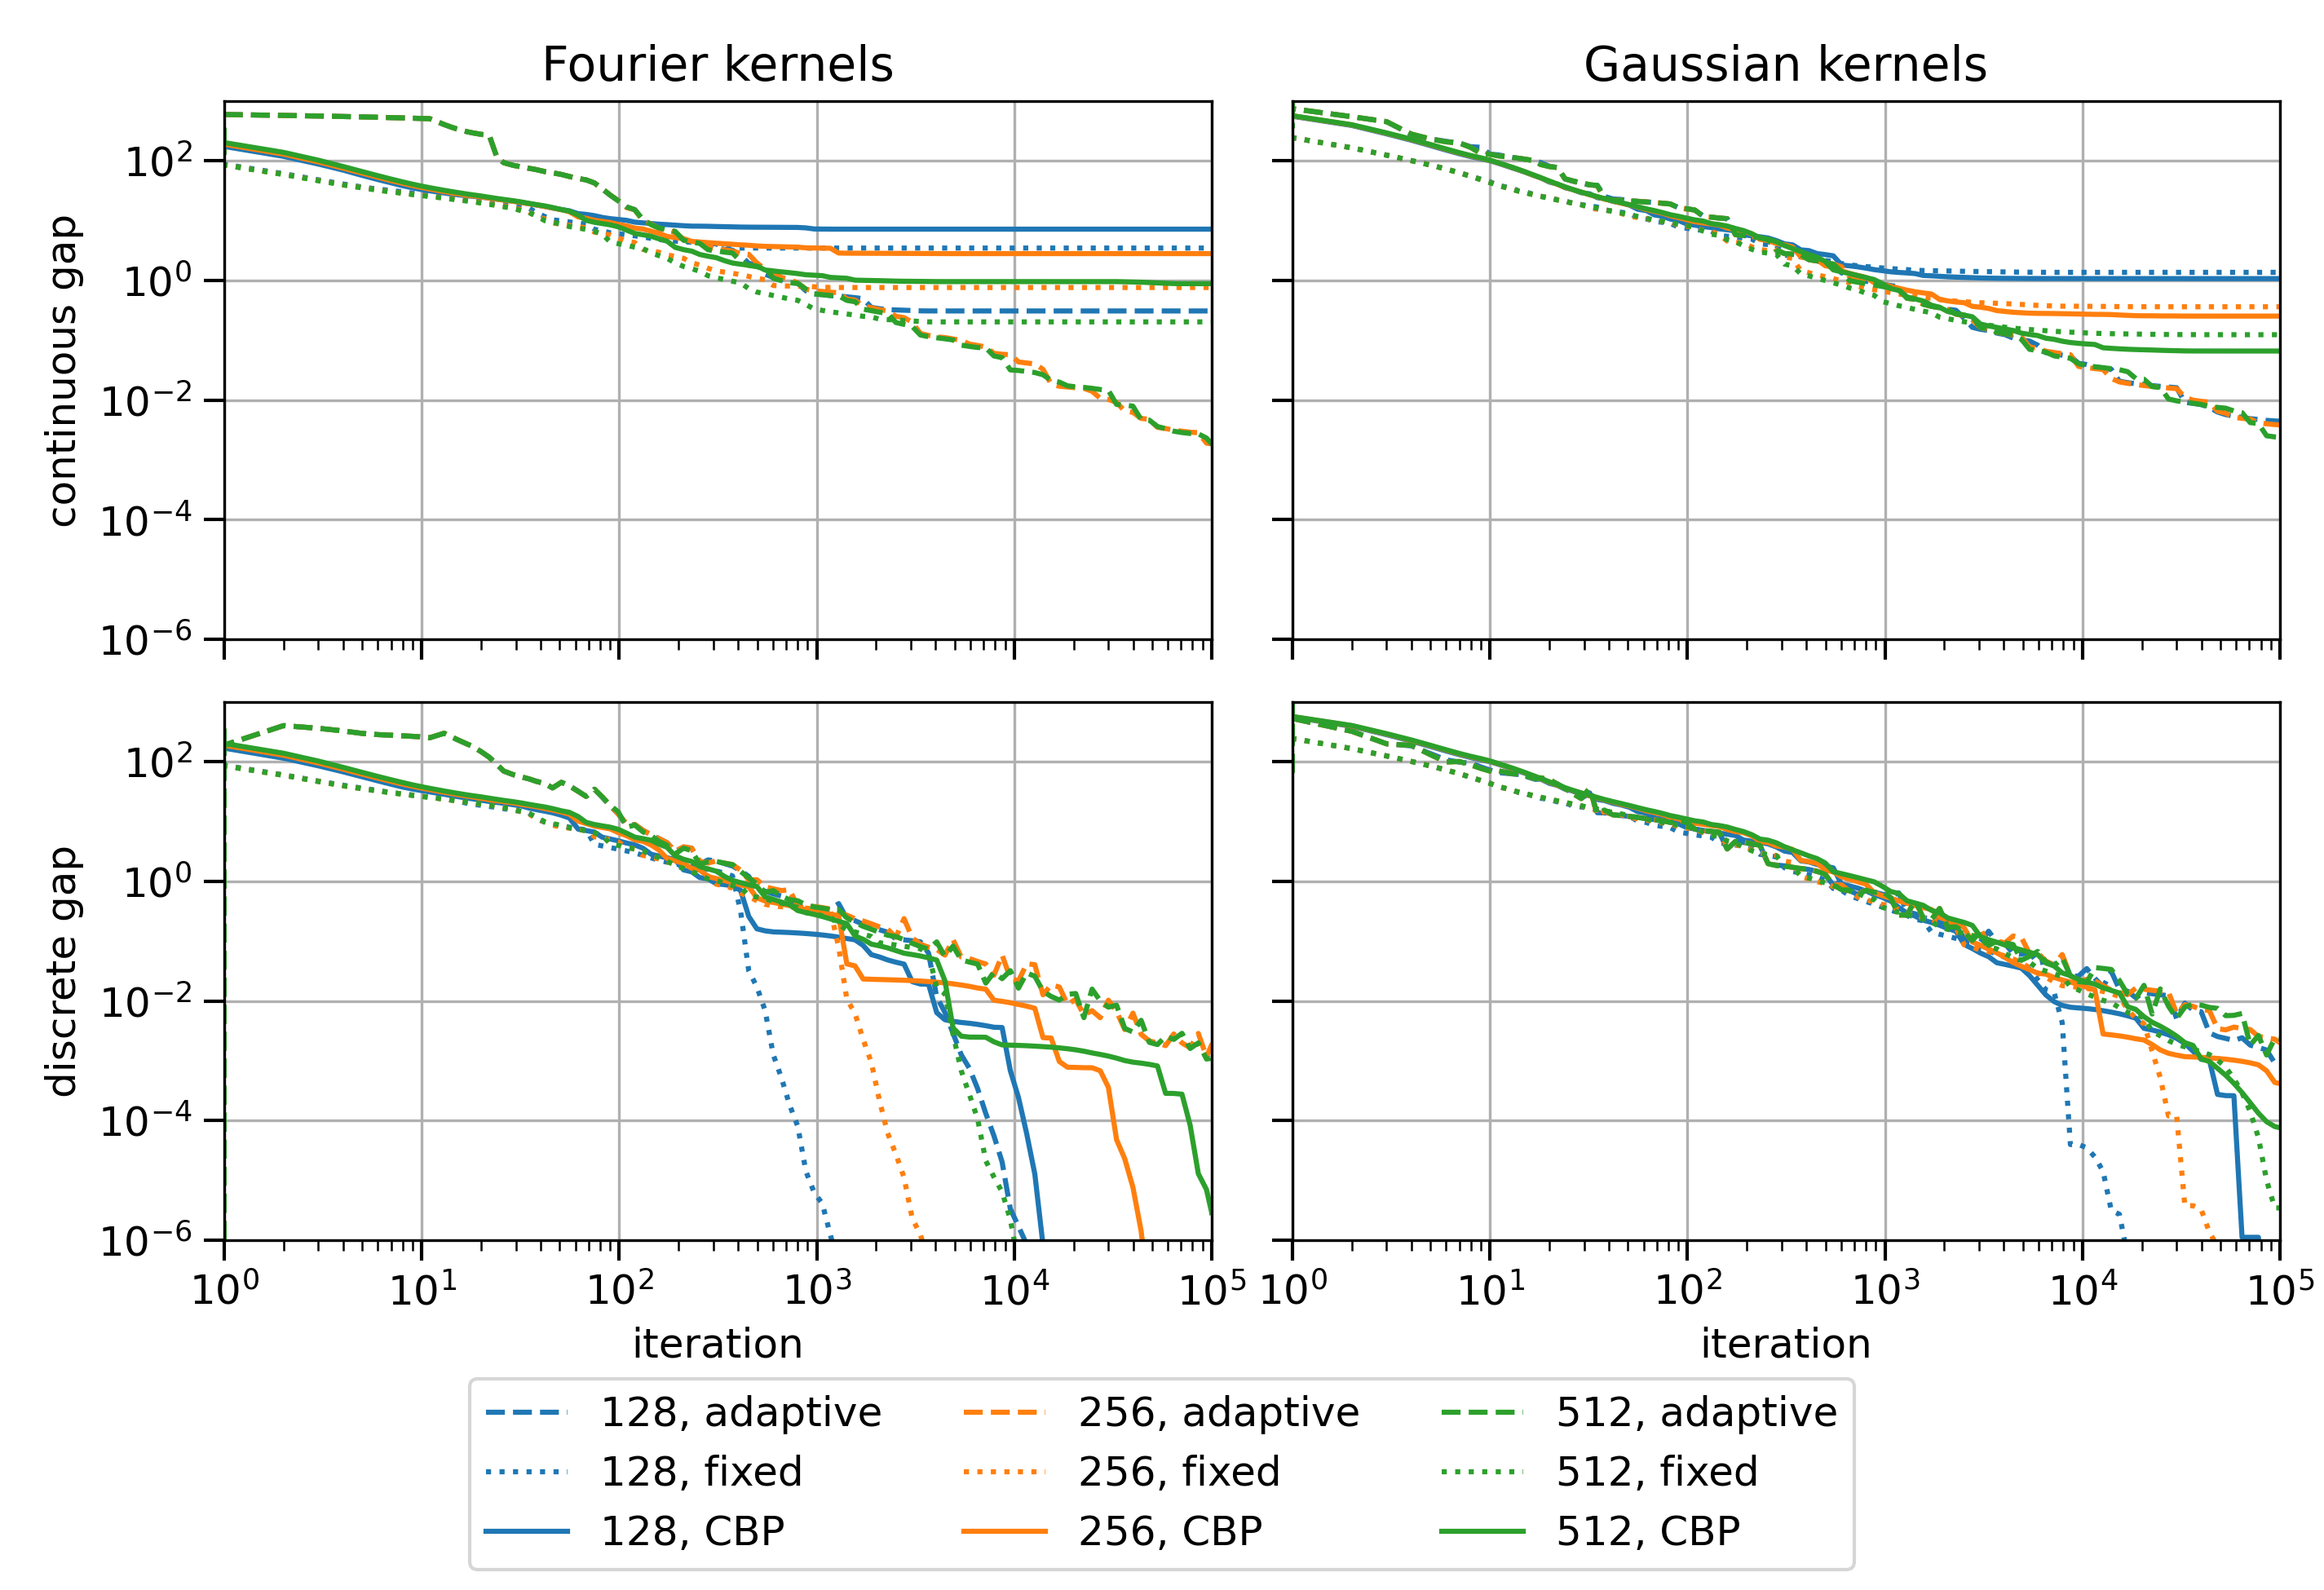
\includegraphics[width=.84\textwidth]{lasso_ndofs_convergence}
	\caption{Rates of continuous/discrete gap convergence for different Lasso algorithms with 128, 256, or 512 pixels. The `adaptive' method uses the proposed algorithm. Both `fixed' and `CBP' use standard FISTA with a uniform discretisation.}\label{fig:ca: convergence with ndofs}
\end{figure}

\paragraph{Comparison of FISTA variants}
There are many variants of FISTA which can also be implemented in the form of \Cref{alg:ca: refining FISTA} just by updating the $\spcf0^n$ on each iteration. Although we have not proven convergence for all of these, \Cref{fig:ca: convergence with method} compares many methods with either fixed or adaptive discretisations. Each adaptive scheme is allowed up to 1024 pixels and each uniform discretisation uses exactly 1024. Forward-Backward splitting (FB) uses a sequence $\vart1_n=1$ otherwise for FISTA a general $\vart1_n = \frac{n+a-1}{a}$ is used. The restarting scheme is given in \Cref{alg:ci: restarting FISTA} and `greedy' FISTA is given in \Cref{alg:ci: greedy FISTA}. In this example CBP used the greedy FISTA implementation which gave faster observed convergence. \Cref{fig:ca: convergence with method} compares the discrete gaps because it is the accurate metric for fixed discretisations, and for the adaptive discretisation it should also be an accurate predictor of the continuous gap. 

\pagebreak The key observations are:
\begin{itemize}
	\item The only algorithm with noticeably different convergence is FB, which is the non-accelerated form of FISTA. Every other algorithm converges at the same approximate rate.
	\item The fixed discretisation schemes have an initial `slow' convergence before reaching a `fast' rate. The solid green line of FISTA $a=2$ appears to achieve the theoretical $\frac1{n^2}$ rate and other FISTA implementations are much faster for large $n$.
	\item During the initial `slow' phase, adaptive and fixed discretisations appear to achieve very similar (discrete) convergence rates. The coarse-to-fine adaptivity is not slower than fixed discretisations in this regime.
	\item \Cref{thm:ca: practical refinement criteria} accurately predicts the $\frac1n$ rate of the adaptive methods, mirrored in the fixed discretisations. This suggests that high-resolution but fixed discretisations are initially limited by the continuous problem before entering the asymptotic discrete regime.
	\item \Cref{thm:ca: practical refinement criteria} only applies to two adaptive schemes, labelled $a=2$ and $a=20$. The remaining FISTA schemes all perform comparably although the restarting scheme is often the slowest. Both $a=20$ and greedy FISTA are consistently the best or near-best performing methods.
\end{itemize}

\begin{figure}[H]\centering
	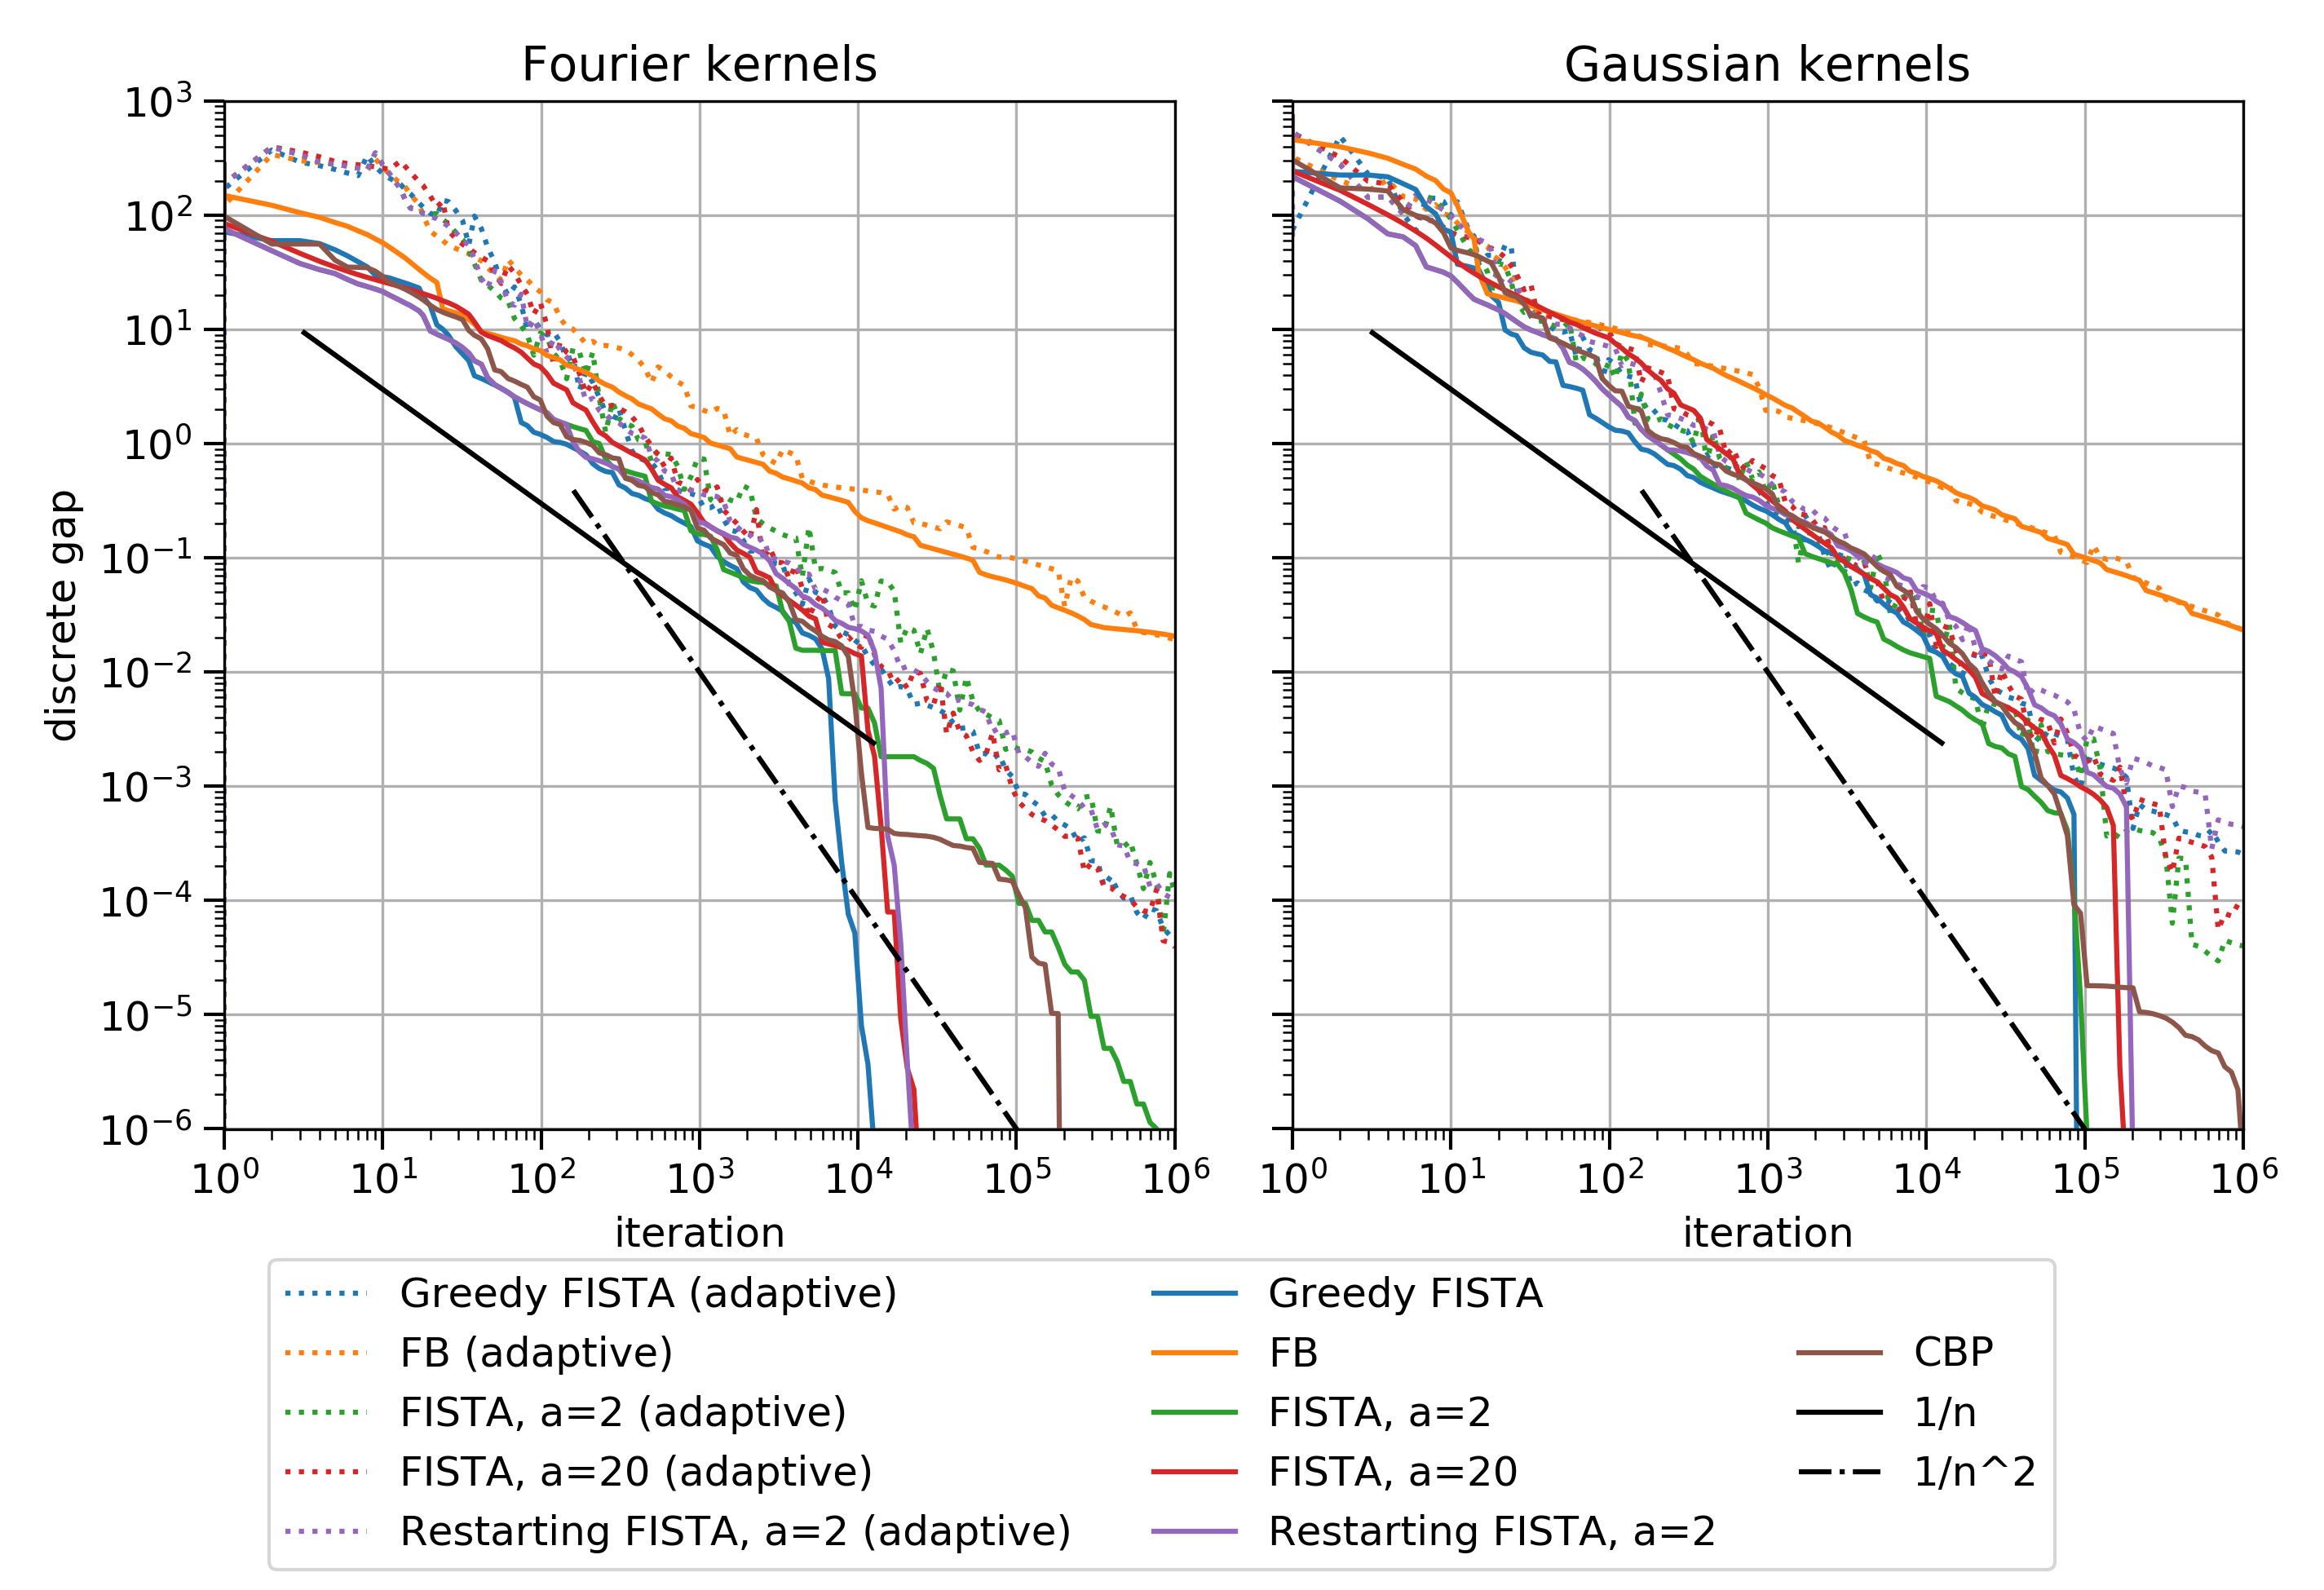
\includegraphics[width=.84\textwidth]{lasso_convergence}
	\caption{Discrete convergence of different algorithms. `Adaptive' methods use \Cref{alg:ca: refining FISTA} with fewer than 1024 pixels and the remaining methods use a uniform discretisation of 1024 pixels.}\label{fig:ca: convergence with method}
\end{figure}

\paragraph{Comparison of fixed and adaptive discretisation}
Motivated by the findings in \Cref{fig:ca: convergence with method}, we now look more closely at the performance of the $a=20$ and the greedy FISTA schemes. We have analytical results for the former but the latter typically performs the best for non-adaptive optimisation and is never worse than $a=20$ in the adaptive setting. We assume that the aim is to find a function $\varf0_n$ with $\Func0_0(\varf0_n)$ smaller than a given threshold. The question is whether it is faster/more efficient to use the proposed adaptive scheme or to use a classical scheme at sufficiently high uniform resolution. The fixed discretisations use 1024 pixels (i.e. uniform pixel size of $2^{-10}$) and the adaptive discretisation starts with two pixels with an upper limit of 1024. 

\Cref{fig:ca: comparison with iteration} shows the convergence with respect to number of iterations. As expected, the fixed discretisation starts with a smaller continuous gap before plateauing to a sub-optimal gap around $\Func0_0=0.1$. In both examples, the greedy FISTA has much faster convergence around $n=100$ and of course the minimum pixel size is constant for the fixed discretisation. 

The adaptive optimisation matches the predicted rates well, both gap and minimum pixel size (equal to $2^{-k}$) decay at a rate of approximately $\frac1n$. Interestingly, in the Fourier case the energy decays a little faster and the resolution is a little slower. This is consistent with $\Func0$ being a little bit smoother than predicted (i.e. $\vars2_{\Func0}>2$). 

It is clear that the adaptive scheme is able to continue reducing the continuous gap far beyond that of the fixed discretisation. The range $n\in[10^3,10^4]$ is particularly interesting because it is the time when the adaptive and fixed curves intersect in both continuous gap and minimum pixel size. Suppose the stopping criterion is to find $\varf0$ such that $\Func0_0(\varf0)<0.1$. \Cref{fig:ca: comparison with iteration} shows that it is equivalent to `guess' the necessary resolution, or to adaptively refine until reaching the stopping criterion. Both methods would converge after $O(10^3)$ iterations with a minimum pixel size of $2^{-10}$.

\Cref{fig:ca: comparison with time} shows a more practical comparison showing wall-clock computation time and number of pixels (memory usage). Optimisation of the fixed discretisation is faster overall but after around \SI{0.1}{\second}, it is always faster to use the adaptive scheme to achieve a given continuous gap. The reason for this can be seen in the numbers of pixels. At the most extreme, in the same computation time the adaptive scheme can achieve more than a factor of 10 better gap using approximately a factor of 10 fewer pixels. The adaptive scheme re-computes the discrete matrix $\A\Pi_n$ each time there is a refinement, but the fixed schemes only compute it once. The adaptive schemes still seem to converge faster than $\frac1{\op{time}}$.

\begin{figure}\centering
	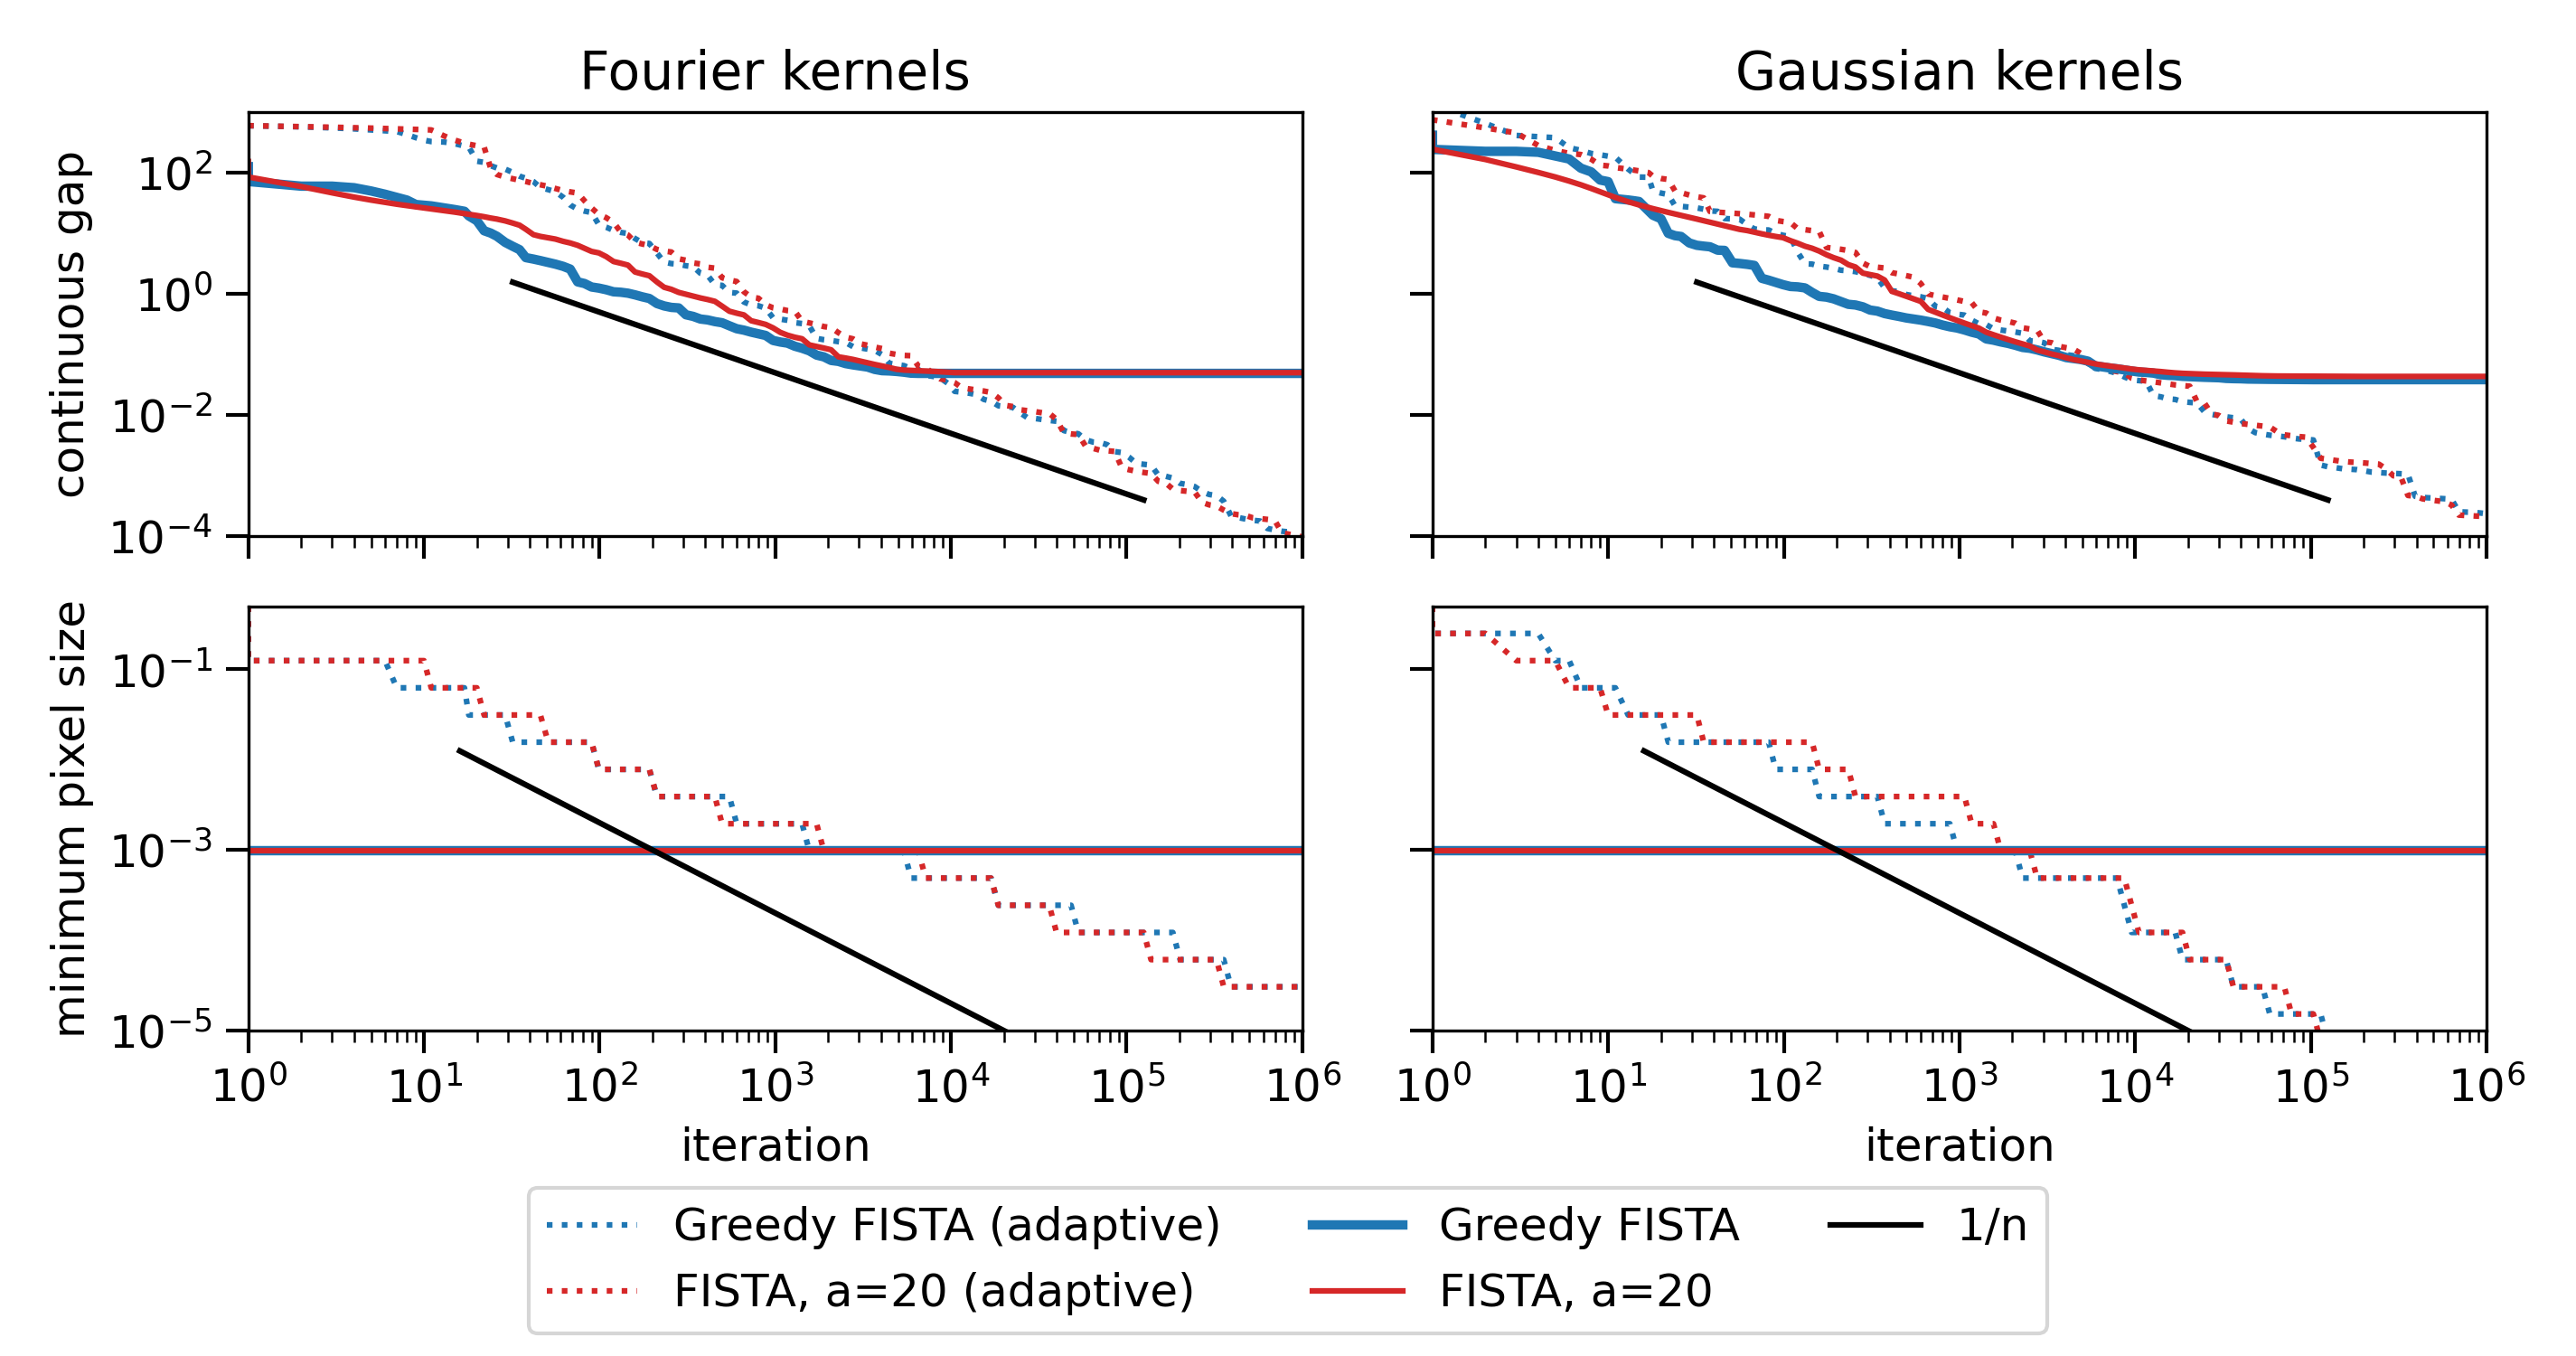
\includegraphics[width=.84\textwidth]{lasso_reduced_convergence}
	\caption{Continuous convergence of adaptive (coarse-to-fine pixel size) compared with uniform discretisation (constant pixel size) with respect to number of iterations. }\label{fig:ca: comparison with iteration}
\end{figure}
\begin{figure}\centering
	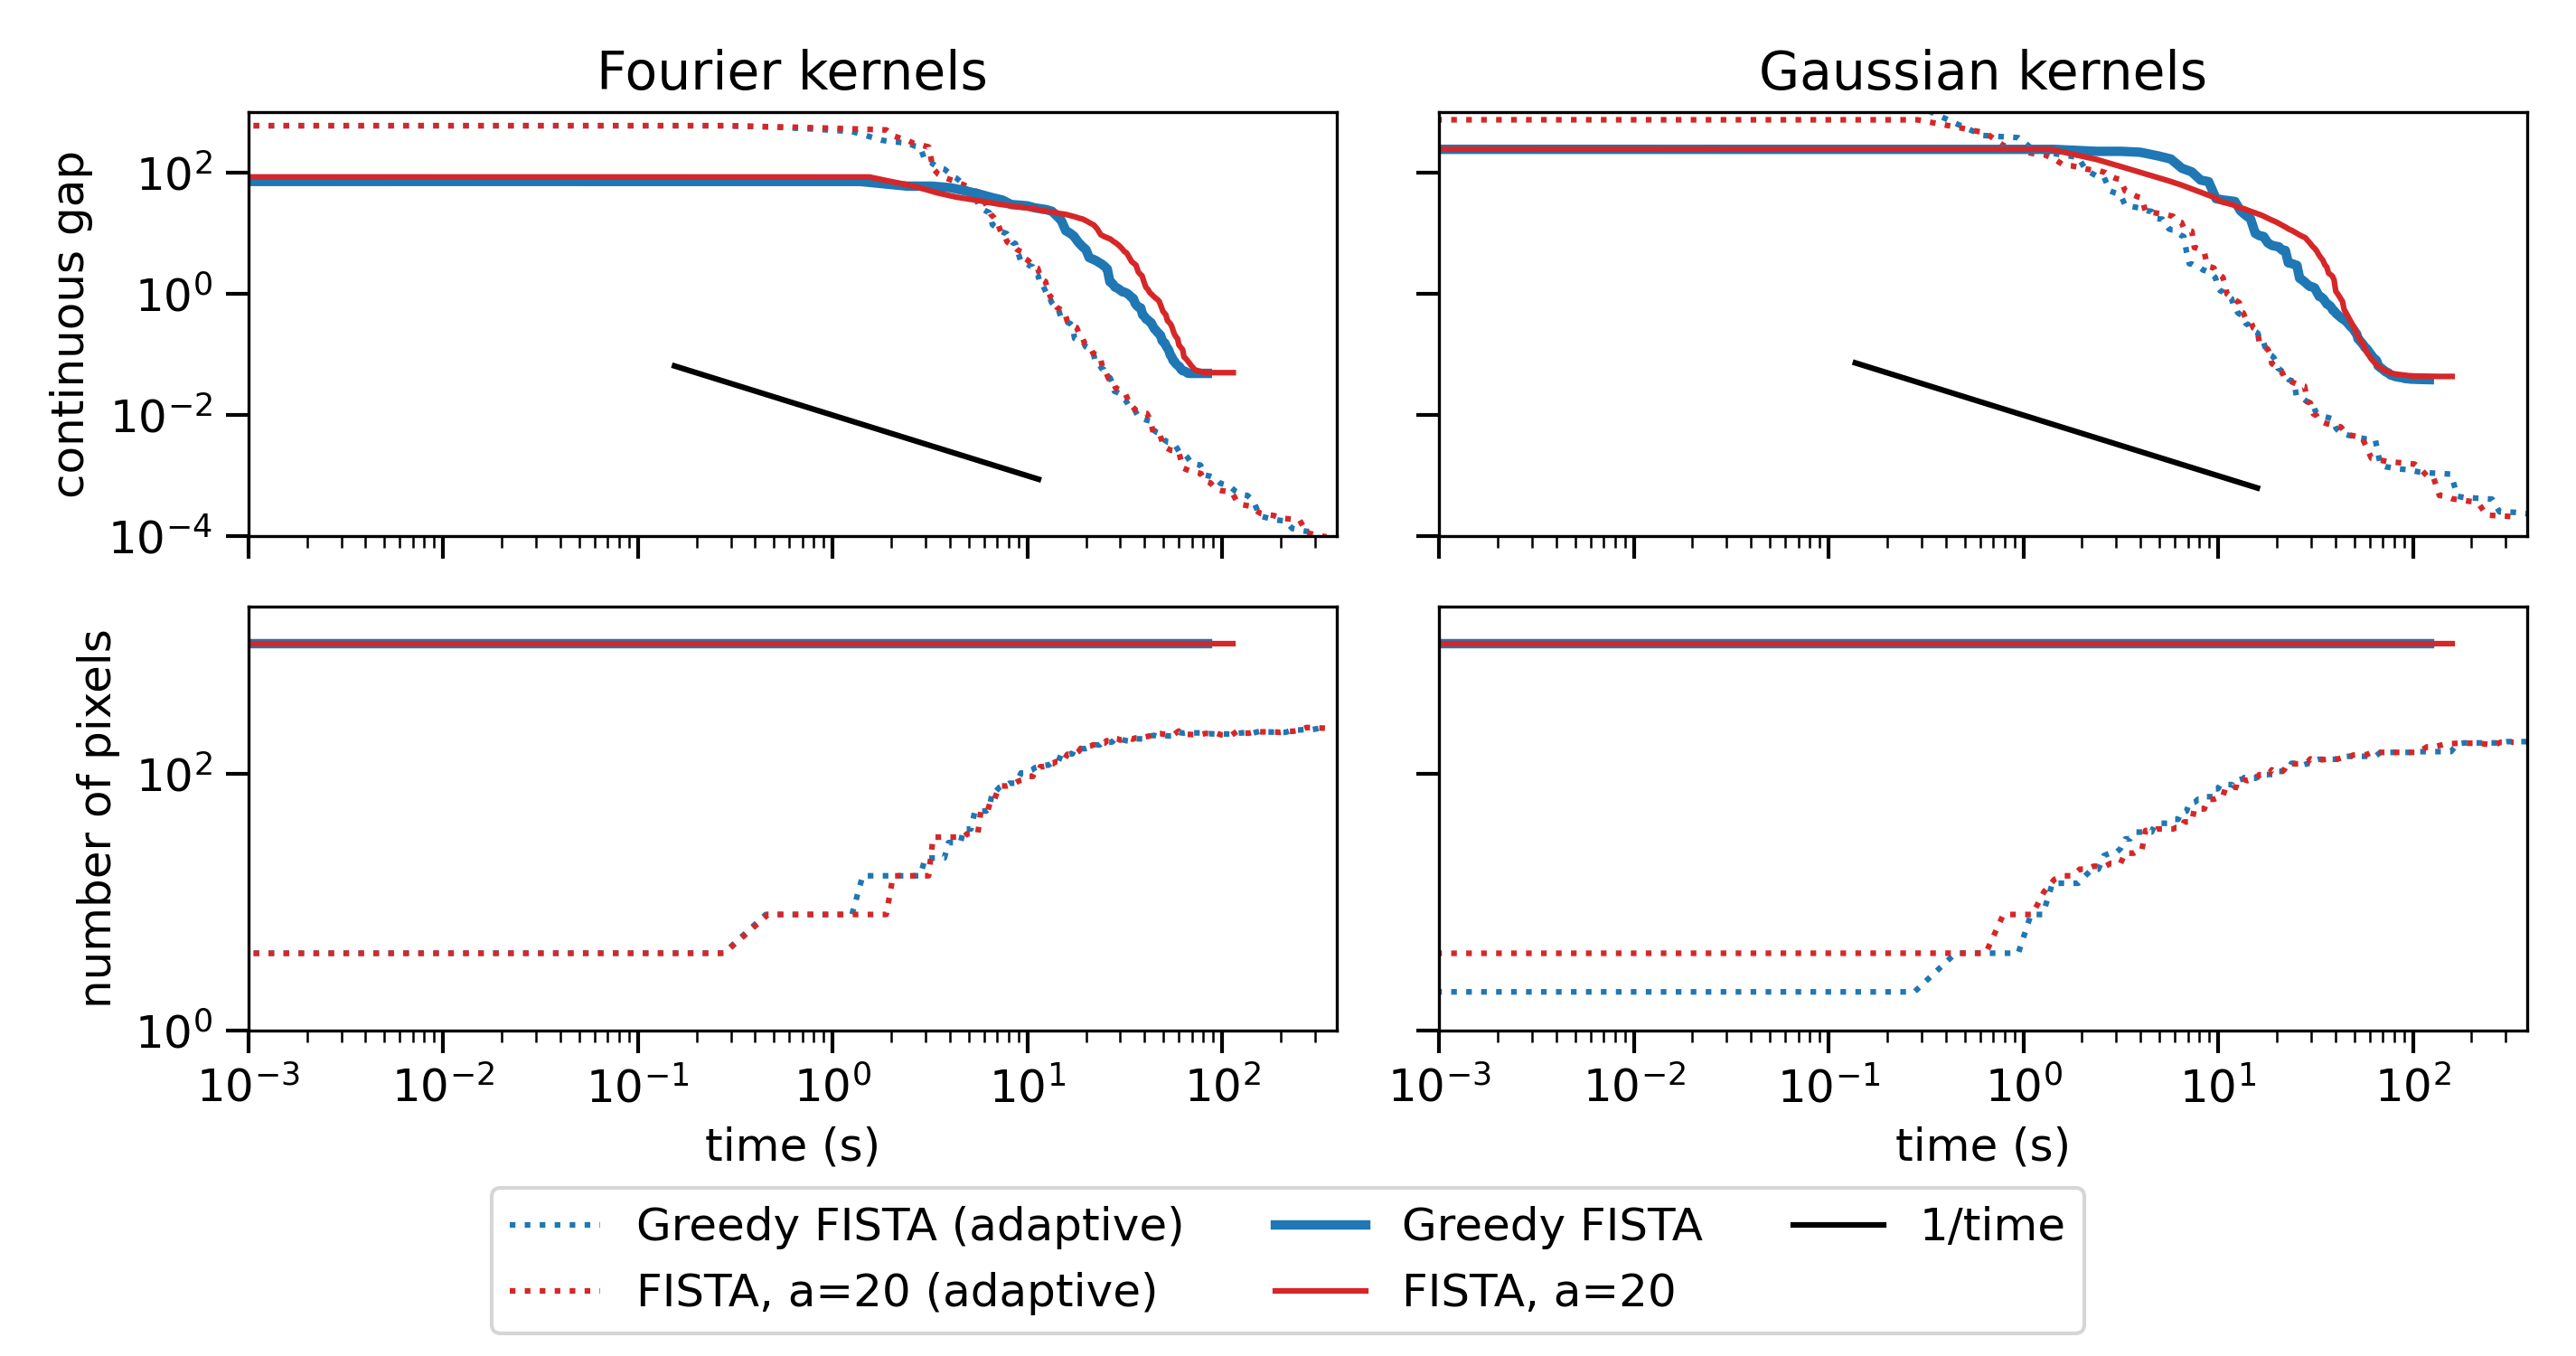
\includegraphics[width=.84\textwidth]{lasso_convergence_time}
	\caption{Continuous convergence of adaptive compared with uniform discretisation with respect to wall-clock time and total number of pixels (memory requirement).}\label{fig:ca: comparison with time}
\end{figure}

\subsection{2D wavelet Lasso}\label{sec:ca: wavelet examples}
In this example we consider $\A$ to be a 2D Radon transform. In particular, the rows of $\A$ correspond to integrals over the sets $\F{\Varx0}^I_i$ where 
$$\F{\Varx0}_i^I = \left\{\vvarx0\in[-\tfrac12,\tfrac12]^2\st \ip{\vvarx0}{\begin{pmatrix}\cos\theta_I\\\sin\theta_I\end{pmatrix}}\in \left[-\tfrac12+\tfrac{i-1}{50},-\tfrac12+\tfrac{i}{50}\right)\right\}, \quad \theta_I=\frac{180^\circ}{51}I \quad \text{ for } i,I\in[50].$$
This is not exactly in the form analysed by \Cref{thm:ca: norm bound examples}, however for each $I$ the sets $\{\F{\Varx0}^I_i\st i\in[50]\}$ are disjoint therefore we can apply \Cref{thm:ca: norm bound examples} block-wise to estimate
$$\norm{\A}_{L^2\to\ell^2} \leq \sqrt{\sum_{I\in[50]}\max_{i\in[50]} |\F{\Varx0}^I_i|} = \sqrt{\sum_{I\in[50]}\max_{i\in[50]} \int_{\F{\Varx0}^I_i}1d\vvarx0}= \sqrt{\sum_{I\in[50]}\max_{i\in[50]}\ (\A\1)_{i,I}}.$$
$\A$ is not smooth, therefore we can't bound $|\A^*|_{C^k}$ for $k>0$, and so we must look to minimise over $\ell^1$ rather than $L^1$. The natural choice is to promote sparsity in a wavelet basis which can be rearranged into the Lasso form:
$$\min_{\varf0\in \spcf0} \tfrac12\norm{\A\varf0-\vdata0}_{\ell^2}^2 + \mu \norm{\linop{W}^{-1}\varf0}_{\ell^1} = \min_{\hat{\varf0}\in\ell^1(\R)} \tfrac12\norm{\A\linop{W}\hat{\varf0}-\vdata0}_{\ell^2}^2 + \mu \norm{\hat{\varf0}}_{\ell^1}.$$
The minimisers are related by $\varf0^* = \linop{W}\hat{\varf0}^*$ and, for wavelet bases, $\linop{W}$ is orthonormal so $\norm{\A\linop{W}}_{\ell^2\to\ell^2} = \norm{\A}_{L^2\to\ell^2}$. From \Cref{sec:ca: Lasso gap and gradient} we know that to track convergence and perform adaptive refinement, it is sufficient to accurately bound $|[\linop{W}^\top \A^*\vvard0_n]_j|$ for all $j\notin J_n$. If $\linop{W}$ is a wavelet transformation then its columns, $w_j\in L^2$, are simply the wavelets themselves and we can use the bound 
\begin{equation*}
	|\IP{w_j}{\A^*\vvard0_n}| = \left|\IP{w_j}{\1_{\supp(w_j)}\A^*\vvard0_n}\right| \leq \norm{\1_{\supp(w_j)} \A^*\vvard0_n}_{L^2}\leq \norm{\1_{\F{\Varx0}} \A^*\vvard0_n}_{L^2}
\end{equation*}
for all $\F{\Varx0}\supset \supp(w_{\vars0})$.
In the case of the Radon transform, we can compute the left-hand side explicitly for the finitely many $j\in J_n$ but we wish to use the right-hand side in a structured way to avoid computing the infinitely many $j\notin J_n$. To do this, we will take a geometrical perspective on the construction of wavelets to view them in a tree format. 

\paragraph{Tree structure of wavelets}
Finite elements are constructed with a mesh which provided a useful tool for adaptive refinement in \Cref{sec:ca: bound continuous}. For wavelets, we will associate a tree with every discretisation and the leaves of the tree form a mesh. This perspective comes from the multi-resolution interpretation of wavelets. We will explain the approach for 1D in detail and then comment on how to extend this picture to higher dimensions. We start with a space $\tilde{\spcf0}^0$ and a normalised mother wavelet $\vard1\colon[0,1]\to \R$ then inductively form $\tilde{\spcf0}^k$ by
$$\tilde{\spcf0}^k = \tilde{\spcf0}^{k-1}\bigcup\left\{w_{j,k}(\varx0) = \sqrt{2}^k\vard1(2^{k}\varx0-j)\st j=0,\ldots 2^k-1\right\}.$$
If we keep track of the support $w_{j,k}$ then we see a tree structure emerging, as shown in \Cref{fig:ca: wavelet tree}.
\begin{figure}\begin{center}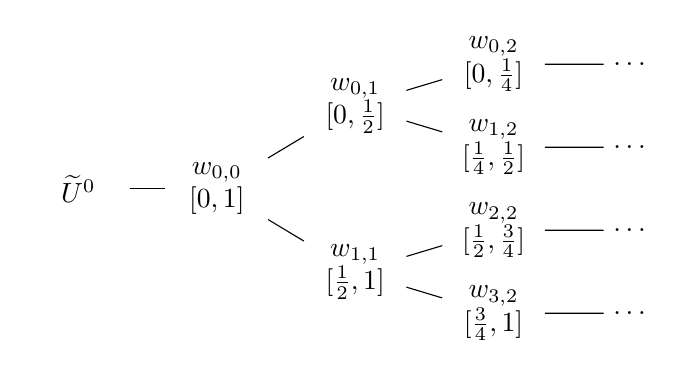
\begin{tikzpicture}[grow'=right]
			\tikzstyle{level 1}=[level distance=5em, sibling distance=0em];
			\tikzstyle{level 2}=[level distance=5em, sibling distance=6em];
			\tikzstyle{level 3}=[level distance=5em, sibling distance=3em];
			\tikzstyle{bag} = [text width=3em, text centered];
			
			\node[bag] {$\tilde{\spcf0}^0$}
			child {node[bag] {$w_{0,0}$ $[0,1]$}
				child {node[bag] {$w_{0,1}$ $[0,\frac12]$}
					child {node[bag] {$w_{0,2}$ $[0,\frac14]$}
						child { node {\ldots} }
					} child {node[bag] {$w_{1,2}$ $[\frac14,\frac12]$}
						child { node {\ldots} }
					}
				} child {node[bag] {$w_{1,1}$ $[\frac12,1]$}
					child {node[bag] {$w_{2,2}$ $[\frac12,\frac34]$}
						child { node {\ldots} }
					} child {node[bag] {$w_{3,2}$ $[\frac34,1]$}
						child { node {\ldots} }
			}}};
	\end{tikzpicture}\end{center}
	\caption{Tree representation of 1D wavelets $w_{j,k}$ are arranged in a tree structure with their support underneath.}\label{fig:ca: wavelet tree}
\end{figure}
Each time a node splits, the support is partitioned exactly between its two children. If we truncate this tree to $J_n$ such that every node either has zero or two children, then the leaves of this tree form a partition of unity. For example
\begin{align*}
	J_n = \{(0,0), (0,1),(1,1), (2,2), (3,2)\} \implies \op{leaf}(J_n) &= \{(0,1), (2,2), (3,2)\}, 
	\\ [0,1] &= [0,\tfrac12]\cup[\tfrac12,\tfrac34]\cup[\tfrac34,1].
\end{align*}
In higher dimensions, the only two things which change are the number of children ($2^d$ for non-leaves) and at each node you store the coefficients of $2^d-1$ wavelets. The support on each node is still a disjoint partition of unity consisting of regular cubes of side length $2^{-k}$ at level $k$. The only change in our own implementation is to translate the support to $[-\tfrac12,\tfrac12]^2$. We briefly remark that the tree structuring of wavelets is not novel and appears more frequently in the Bayesian inverse problems literature, for example in \cite{Castillo2019}.

\paragraph{Continuous gradient estimate}
In \Cref{sec:ca: 1D Lasso examples} we used the continuous gap as a measure for convergence, for wavelets we will use the continuous gradient. With the tree structure we can easily adapt the results of \Cref{sec:ca: Lasso gap and gradient} to estimate gradients (or function gaps). In particular,
\begin{align}
	\Norm{\partial \Func0(\varf0_n)}_* &=\max\left(\Norm{\partial_n\Func0(\varf0_n)}_*, \max_{j\notin J_n} |\IP{w_j}{\A^*\vvard0_n}| -\mu \right) \\&\leq\max\left(\Norm{\partial_n\Func0(\varf0_n)}_*, \max_{j\in \op{leaf}(J_n)} \norm{\1_{\supp(w_j)}\A^*\vvard0_n}_{L^2} -\mu \right).\label{eq:ca: wavelet error metric}
\end{align}
It is interesting to note that 
$$\sum_{j\in\op{leaf}(J_n)} \norm{\1_{\supp(w_j)}\A^*\vvard0^*}_{L^2}^2 = \norm{\A^*\vvard0^*}_{L^2}^2,$$
therefore the task of refinement is somehow to partition the domain of $\A^*\vvard0^*$ such that no single component has more than $\mu$ magnitude. Also, by strong convexity of the dual problem,
$$\left|\vars2_0\norm{\1_{\supp(w_j)}\A^*\vvard0_n}_{L^2} - \norm{\1_{\supp(w_j)}\A^*\vvard0^*}_{L^2}\right| \leq \sqrt{|\supp(w_j)|}\sqrt{2(\Func0(\varf0_n)+\Func0^*(\vars2_0\vvard0_n))},$$
therefore the exact discretisation is reached in finite time. After this point, the discretised problem is equal to the continuous problem, and \Cref{alg:ca: refining FISTA} will behave as in the classical setting.

\paragraph{Numerical results}
We consider two phantoms where $\varf0^\dagger$ is either a binary disc or the Shepp-Logan phantom. No noise is added to the Shepp-Logan data but \SI{5}{\percent} Gaussian white noise is added to the disc data. This is visualised in \Cref{fig:ca: haar data}. All optimisations shown will be spatially adaptive using Haar wavelets and initialised with four degrees of freedom (denoted $\spcf0^1$ in the notation of \Cref{fig:ca: wavelet tree}). The gradient metric shown throughout is the $\ell^2$ norm. Motivated by \eqref{eq:ca: wavelet error metric}, the spatial adaptivity is chosen to refine nodes $j\in\op{leaf}(J_n)$ such that 
$$ \norm{\1_{\supp(w_j)}\A^*\vvard0_n}_{L^2} -\mu  \leq 10\Norm{\partial_n\Func0(\varf0_n)}_*,$$
i.e. so that the continuous gradient is less than 10 times the discrete gradient.

\begin{figure}[H]\centering
	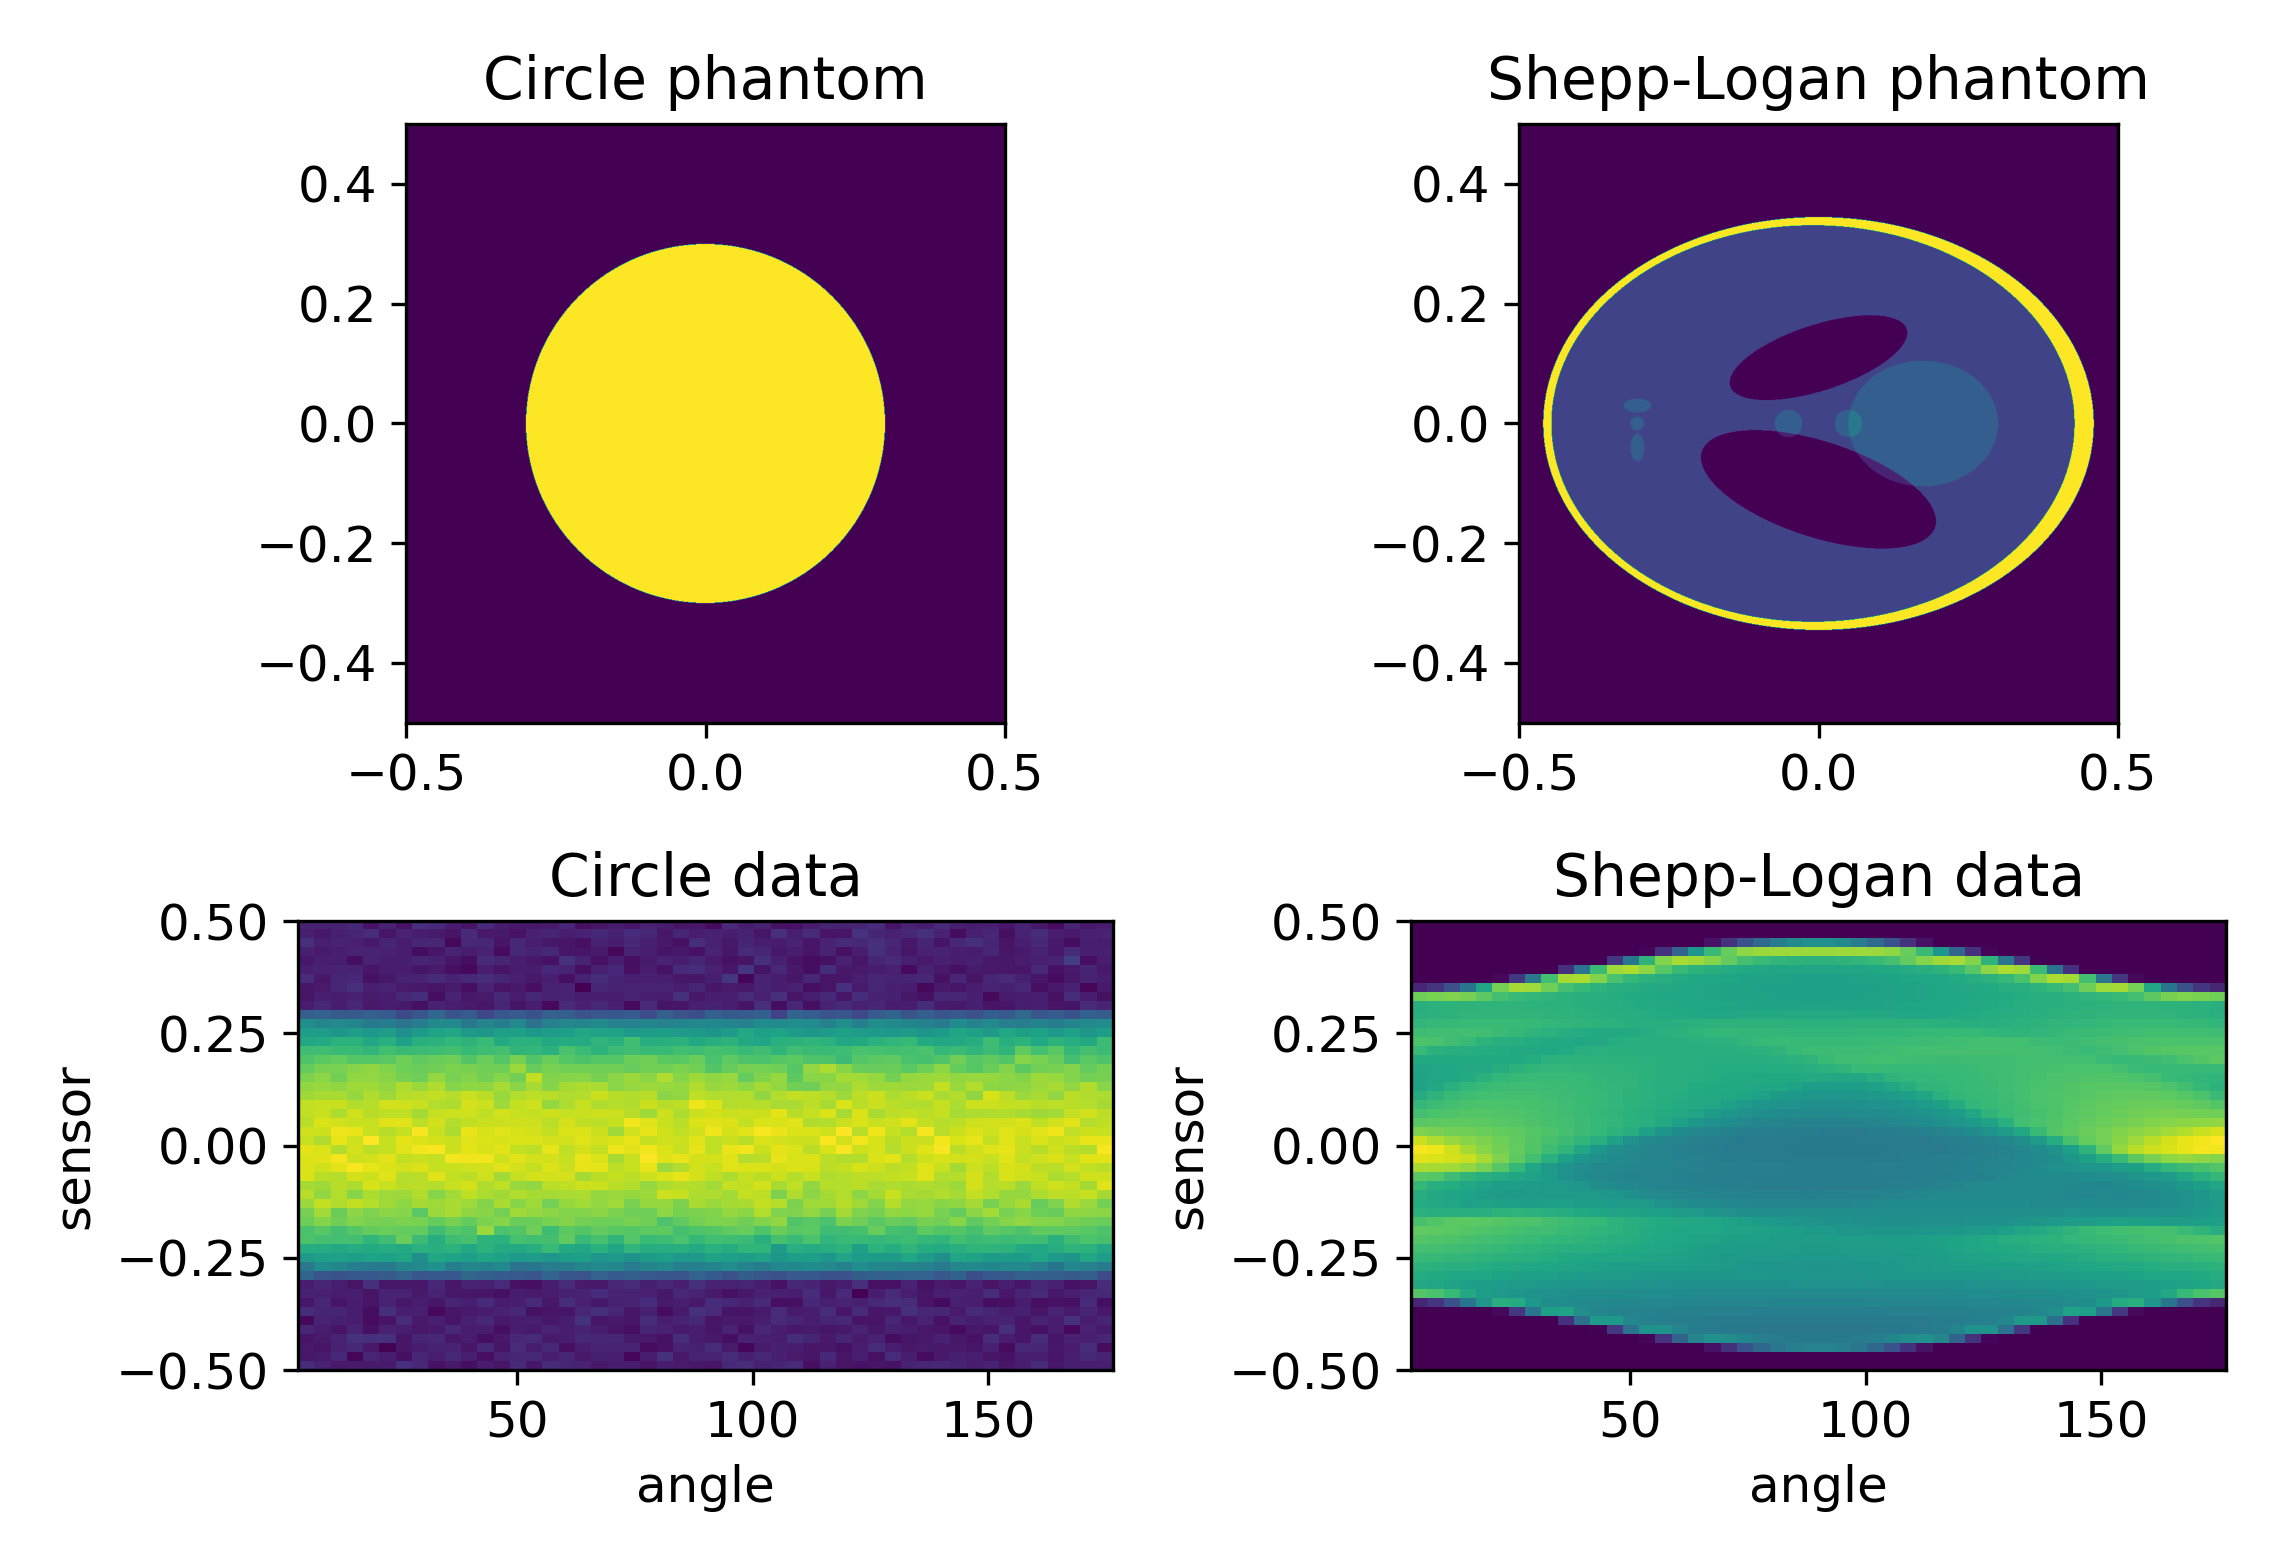
\includegraphics[width=.84\textwidth]{haar_data}
	\caption{Phantoms and data used for wavelet-sparse tomography optimisation. The Shepp-Logan data is exact but the data for the disc-phantom has \SI{5}{\percent}\ Gaussian white noise. Without noise the data would be uniform with respect to the angle.}\label{fig:ca: haar data}
\end{figure}

The first numerical results shown in \Cref{fig:ca: haar convergence} compare the same adaptive algorithms as shown in \Cref{fig:ca: convergence with method}. In these examples we see that the greedy FISTA, restarting, and the $a=20$ algorithms achieve almost linear convergence while $a=2$ and the classical FB are significantly slower. The maximum number of wavelet coefficients used was 312,220 and 44,644 for the circle and Shepp-Logan phantoms respectively.

\begin{figure}[H]\centering
	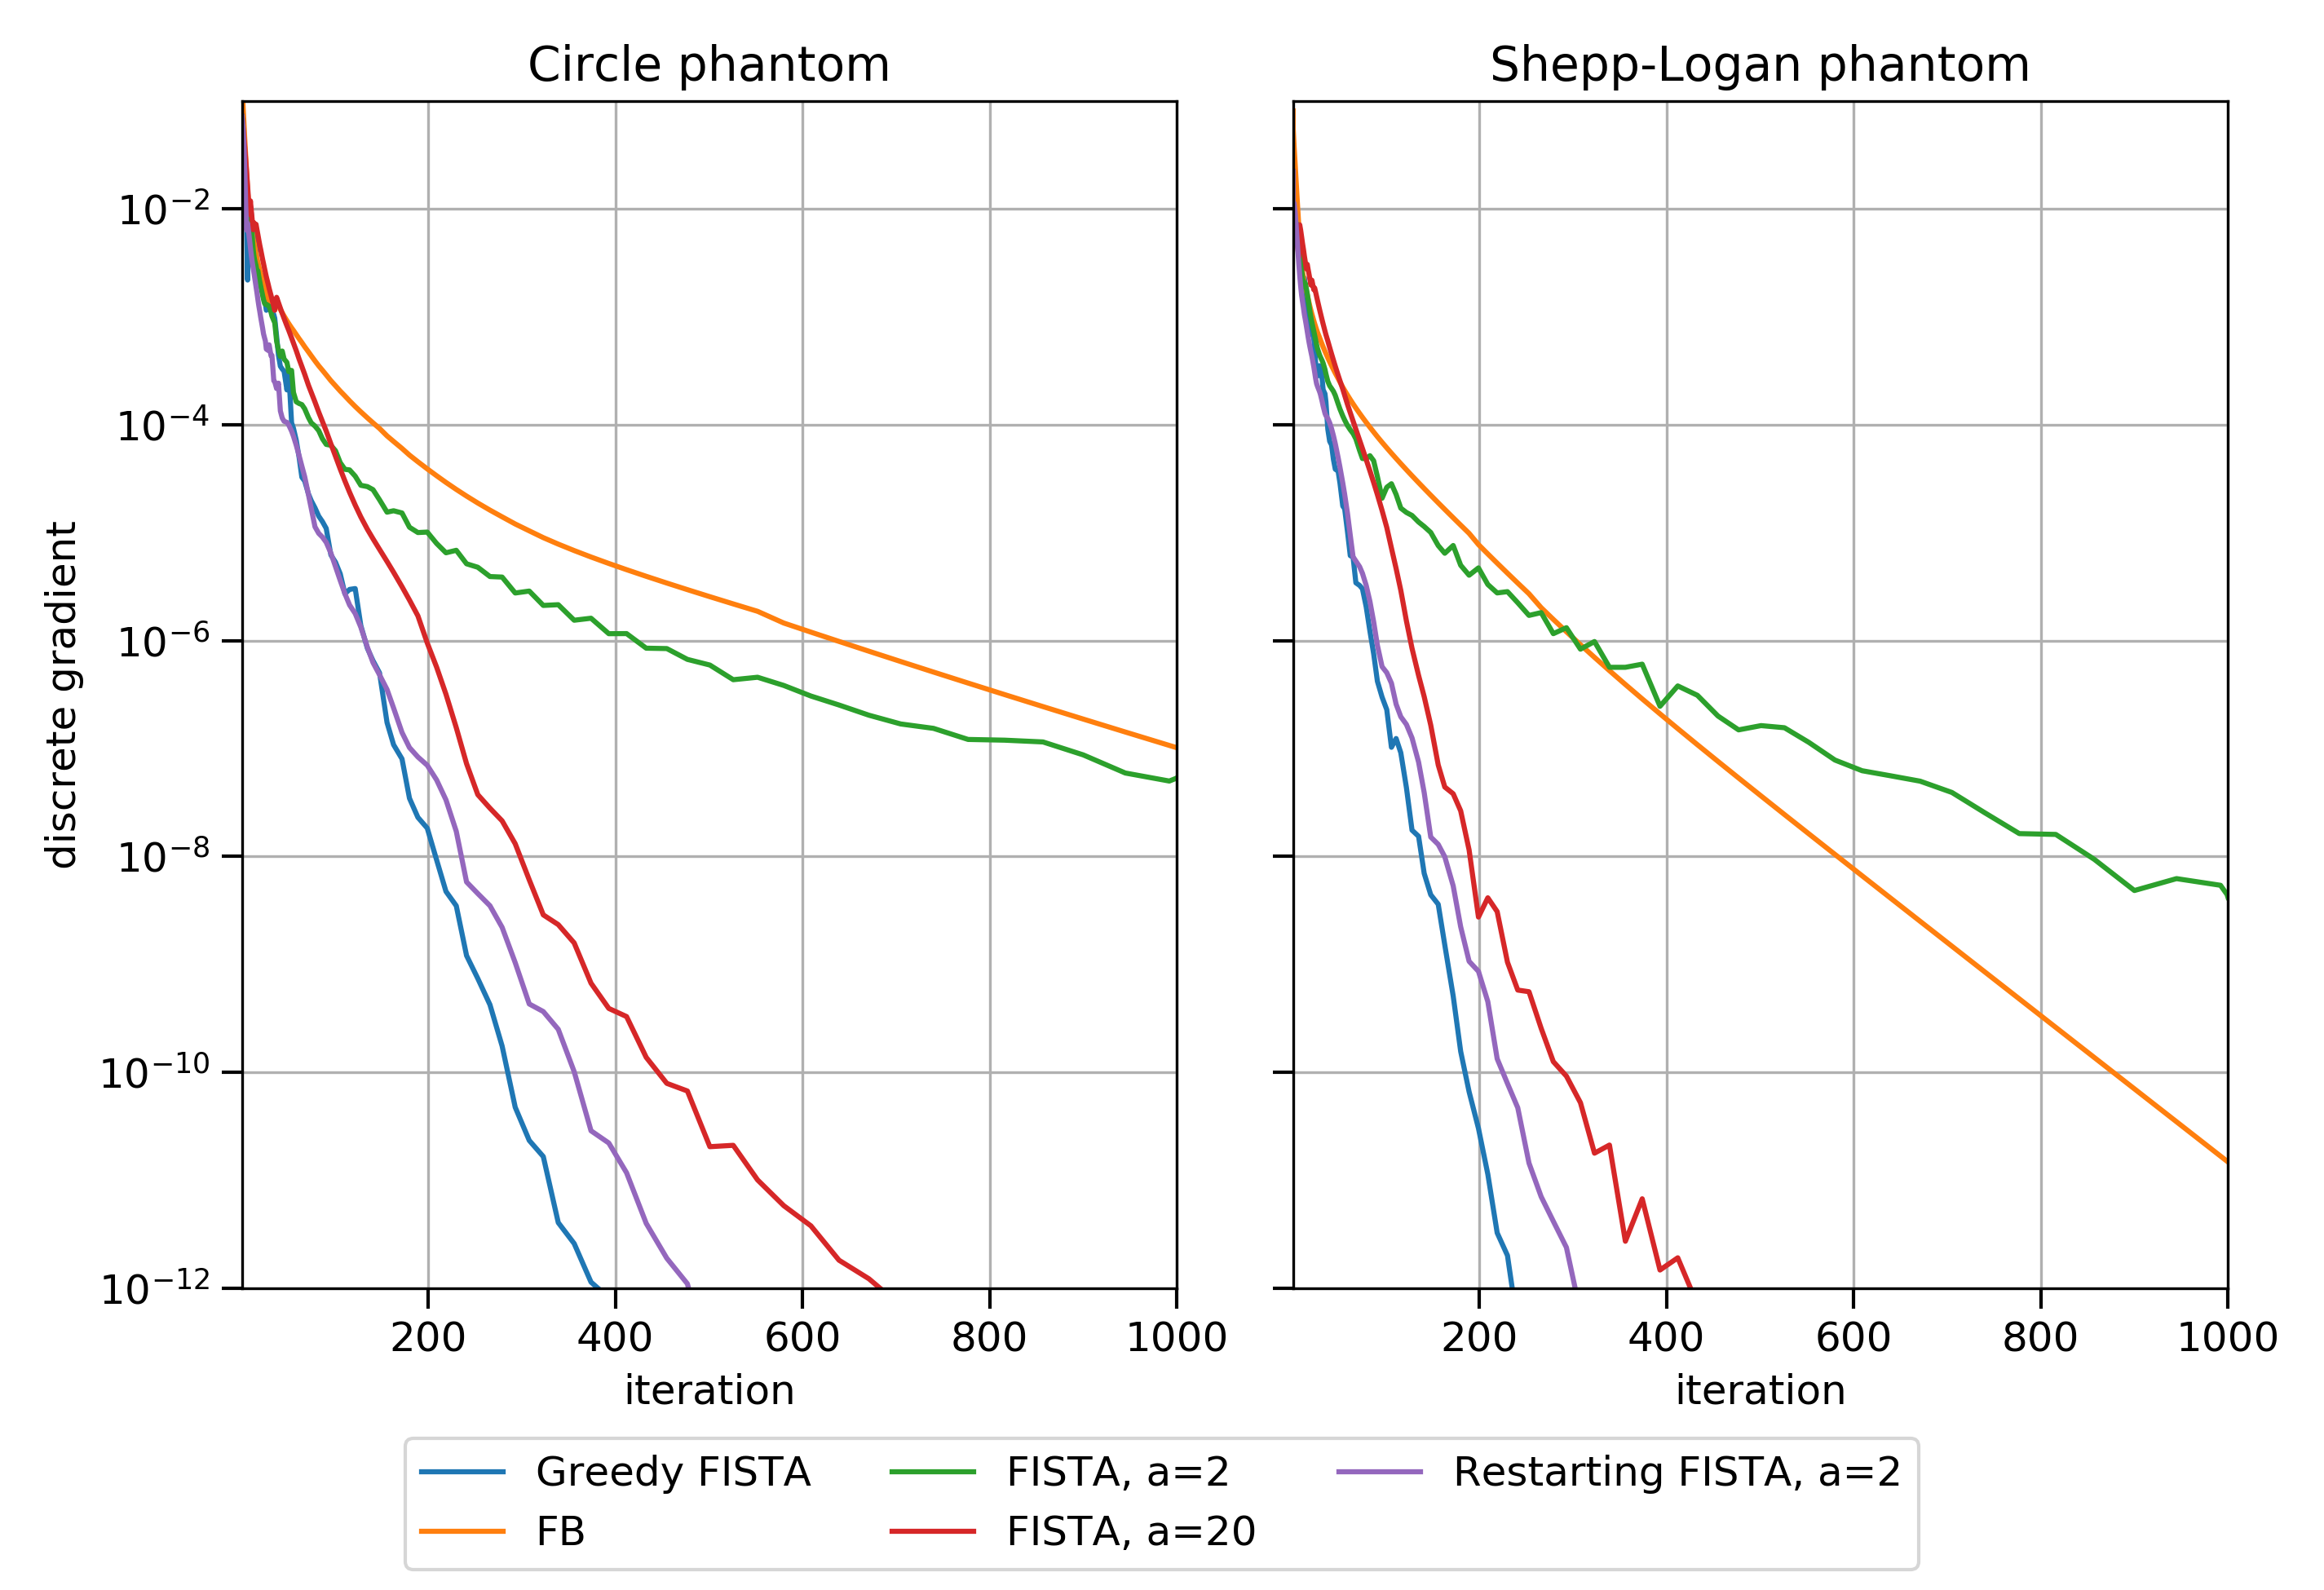
\includegraphics[width=.84\textwidth]{haar_convergence}
	\caption{Discrete convergence of different implementations of \Cref{alg:ca: refining FISTA} with an unlimited number of pixels.}\label{fig:ca: haar convergence}
\end{figure}

As before, we focus on the $a=20$ algorithm to which \Cref{thm:ca: practical refinement criteria} applies, and greedy FISTA which we see achieves slightly faster convergence in \Cref{fig:ca: haar convergence zoom}. Looking at the discrete and continuous gradient norms, we see that they are initially distinct then merge after around 50 iterations. From this point onwards, the continuous and discrete problems are equivalent and the iterations are equivalent to classical FISTA.

\begin{figure}\centering
	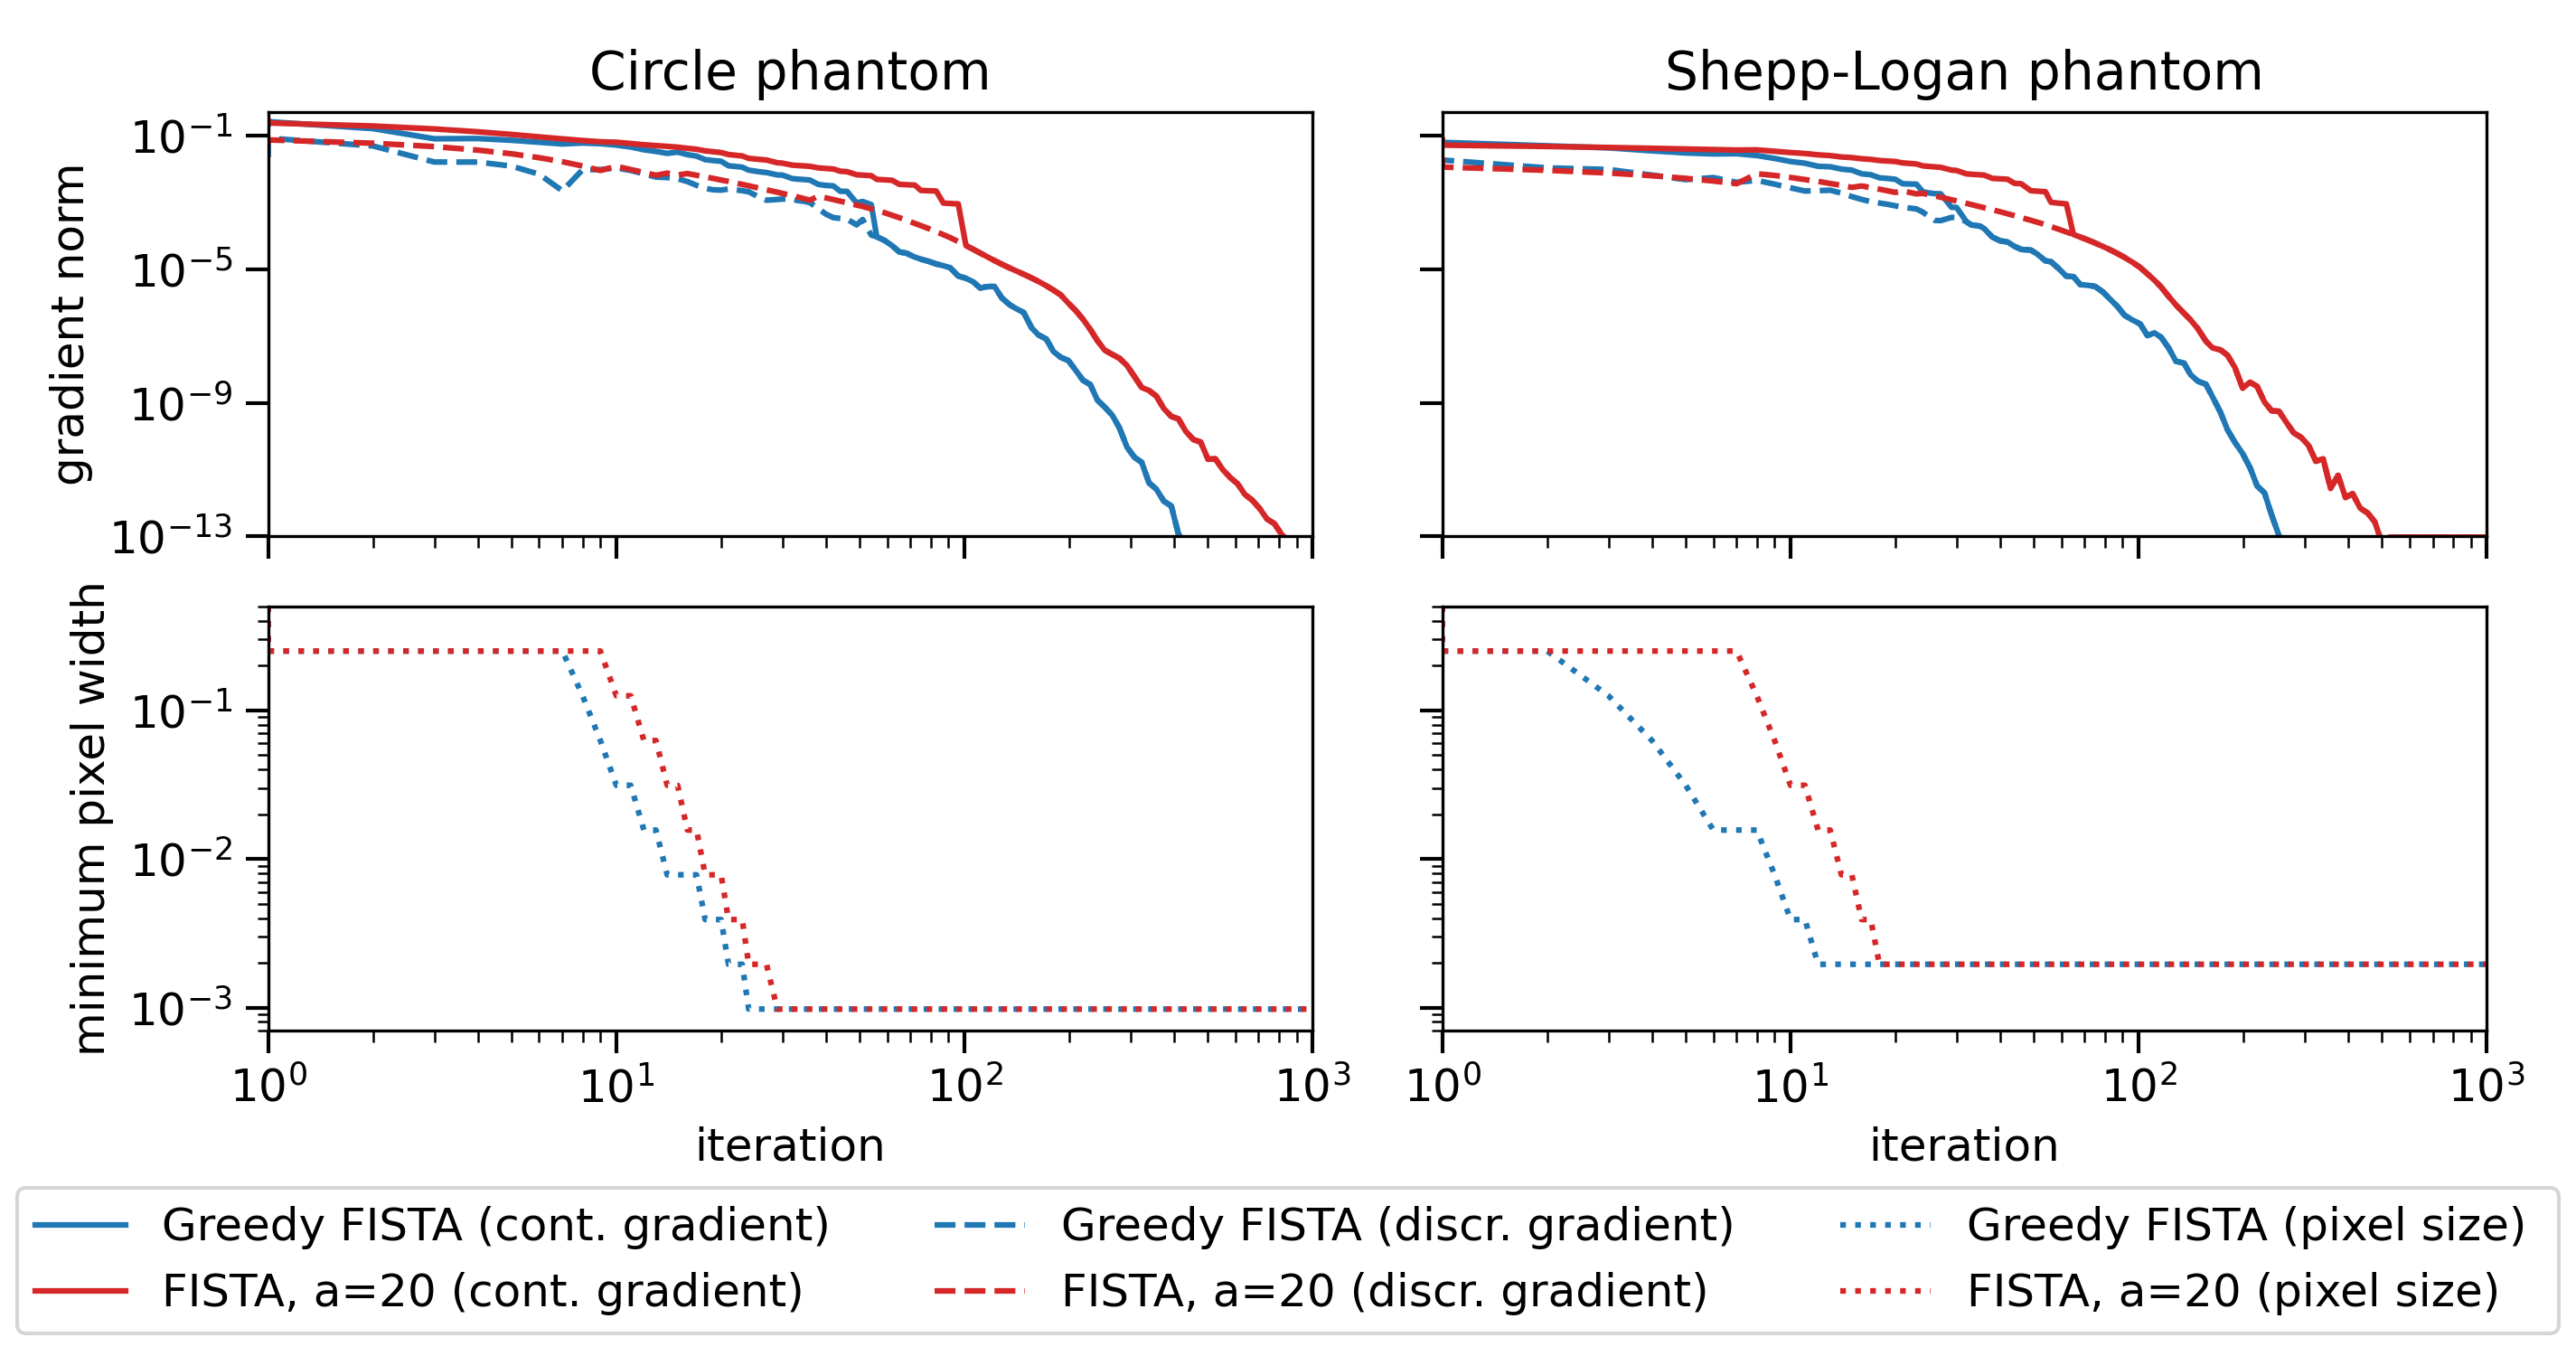
\includegraphics[width=.84\textwidth]{haar_reduced_convergence}
	\caption{Discrete/continuous convergence of adaptive FISTA algorithms on the wavelet Lasso optimisation.}\label{fig:ca: haar convergence zoom}
\end{figure}

\subsection{2D continuous Lasso}
Our final application is a super-resolution/de-blurring inverse problem from biological microscopy. The resolution of visible light microscopy is fundamentally limited by the wavelength of visible light. Classically, this limit has held around \SI{250}{\nano\meter}, however, in recent years new techniques have emerged improving resolution to around \SIrange{30}{50}{\nano\meter} \cite{Schermelleh2019}. A big component of this shift is a growing reliance on more powerful data processing techniques. \emph{Stochastic Optical Reconstruction Microscopy} (STORM) is an example of \emph{Single Molecule Localisation Microscopy} (SMLM) where a large number of coarse blurred images are recorded, then re-combined to form a single sparse super-resolved image. In the context of STORM, each recorded image is modelled as a sparse signal convolved with a point-spread function, then corrupted with noise. The Lasso formulation has previously been shown to be effective in the context of STORM \cite{Huang2017,Denoyelle2019}.

In this example we use a simulated dataset provided as part of the 2016 SMLM challenge\footnote{\url{http://bigwww.epfl.ch/smlm/challenge2016/datasets/MT4.N2.HD/Data/data.html}} for benchmarking software in this application. It is common to model the point-spread function as a Gaussian, in this example the corresponding Lasso formulation  is 
$$ (\A\varf0)_{i} = (2\pi\sigma^2)^{-1}\int_{[0,6.4]^2} \exp\left(-\frac{1}{2\sigma^2}\left|\vvarx0- \Delta\begin{pmatrix}i_1+\tfrac12 & i_2+\tfrac12\end{pmatrix}^\top \right|^2\right)\varf0(\vvarx0)$$
where $\sigma=\SI{0.2}{\micro\meter}$, $\Delta=\SI{0.1}{\micro\meter}$, and $i_1,i_2\in[64]$ where $\spcf0=\C M([\SI{0}{\micro\meter},\SI{6.4}{\micro\meter}]^2)$. 3020 frames are provided, examples of which are shown in \Cref{fig:ca: STORM data}. To process this dataset, image intensities were normalised to $[0,1]$ then a constant was subtracted to approximate 0-mean noise. The greedy FISTA algorithm was used for optimisation with $\mu=0.15$, $10^3$ iterations, and a maximum of $10^5$ pixels per image. 

Finally, all the reconstructions were summed and the result shown in \Cref{fig:ca: STORM results}. The average pixel width after optimisation was approximately \SI{2.4}{\nano\meter}, a factor of 40 super-resolution. If this resolution had been implemented with a uniform discretisation then it would have required $70\times 10^5$ pixels, nearly a factor of 100 greater than achieved with the adaptive discretisation. Lasso is compared with ThunderSTORM \cite{Ovesny2014}, a popular ImageJ plugin \cite{Schindelin2012} which finds the location of signal using Fourier filtering. The performance of ThunderSTORM was rated very highly in the initial competition by \cite{Sage2015}. Both methods compared here demonstrate the key structures of the reconstruction, however, both are sensitive to tuning parameters. In this examples, Lasso has possibly recovered too little signal and ThunderSTORM contains spurious signal. 

\Cref{fig:ca: STORM convergence} shows the convergence behaviour in this example. The estimates given by \eqref{eq:ca: Lasso energy rate} and \eqref{eq:ca: Lasso resolution rate} in dimension $d=2$ predict respectively that the adaptive energy will decay at a rate of $\Func0_0(\varf0_n)\lesssim n^{-\sfrac23}$ so long as the pixel size also decreases at a rate of $\meshsize\sim n^{-\sfrac23}$. This is consistent with the resolution scaling (middle panel) but the energy (left panel in pink) is observed to converge a little faster than predicted. 

In this example we also implement the suggestion of \Cref{sec:ca: support detection} to remove pixels from the iteration once we can guarantee they are outside of the support. \eqref{eq:ca: support equation} provides a threshold to identify the support of the discrete/continuous minimiser and the value of this is plotted in the first panel of \Cref{fig:ca: STORM convergence}, in particular the normalised value $1-\frac{\op{threshold}}{\mu}$ which converges to 0 for large $n$. Any pixel $\domain_i^n$ satisfying 
$$ \vars2_0\norm{\Pi_n\A^*\vvard0_n}_{L^\infty(\domain_i^n)} \leq \op{threshold}$$
guarantees that $\domain_i^n\cap\op{supp}(\varf0^*) = \emptyset$. Once this threshold becomes greater than 0 (plotted value less than 1), we can start reducing the number of pixels instead of just continual refinement. We can see this in the right-hand panel of \Cref{fig:ca: STORM convergence}, after around 30 iterations the total number pixels starts to reduce and stabilise at approximately $6\times10^3$ pixels per frame, well below the upper limit of $10^5$.

\begin{figure}\centering
	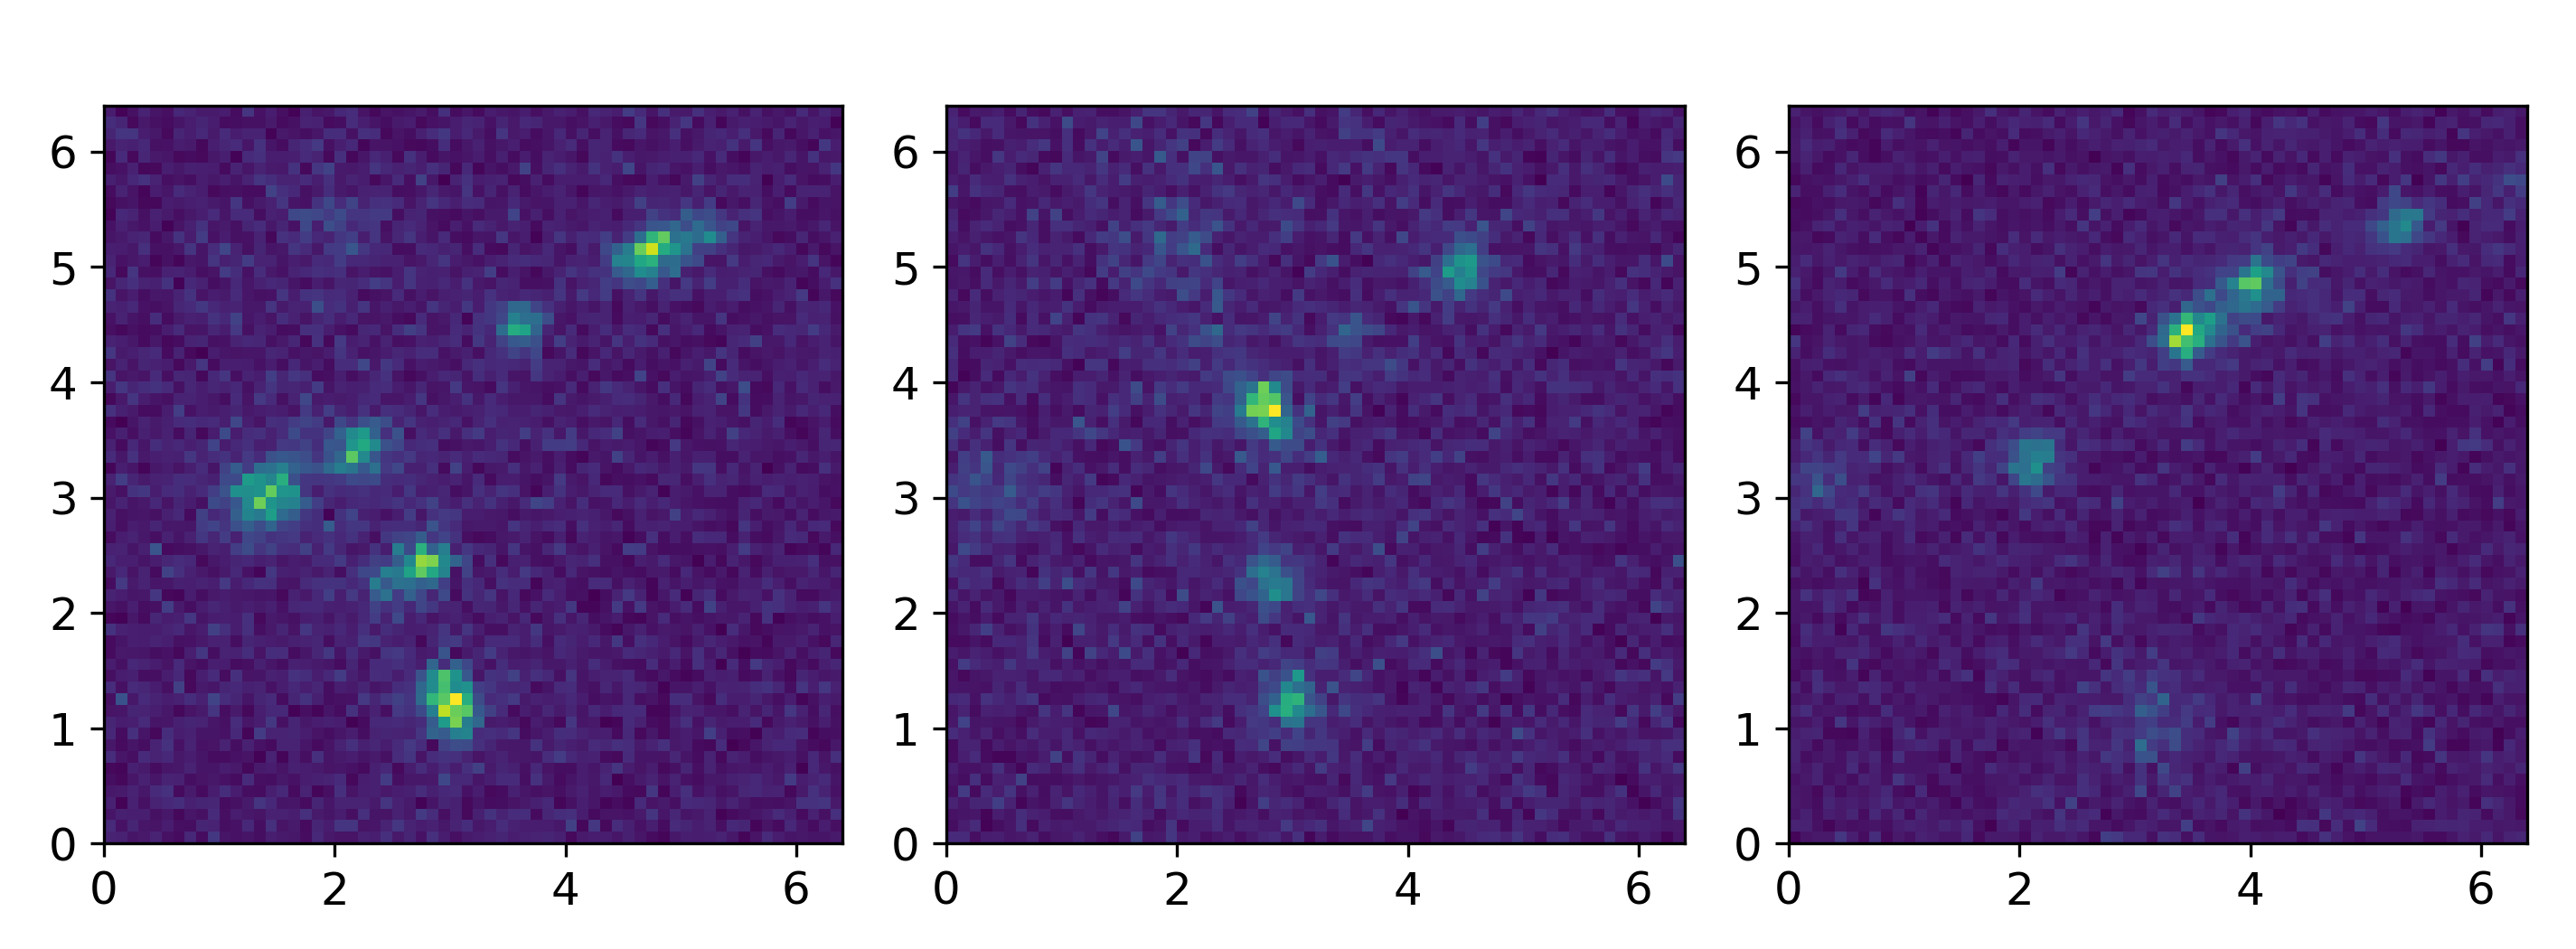
\includegraphics[width=.8\textwidth]{STORM_data}
	\caption{Example of images from STORM dataset.}\label{fig:ca: STORM data}
\end{figure}
\begin{figure}\centering
	\includegraphics[width=.77\textwidth]{STORM_recon}
	\caption{Processed results of the STORM dataset. Top left: Lasso optimisation with \Cref{alg:ca: refining FISTA}. Top right: Comparison with ThunderSTORM plugin. Bottom: Average data, no super-resolution or de-blurring.}\label{fig:ca: STORM results}
\end{figure}
\begin{figure}\centering
	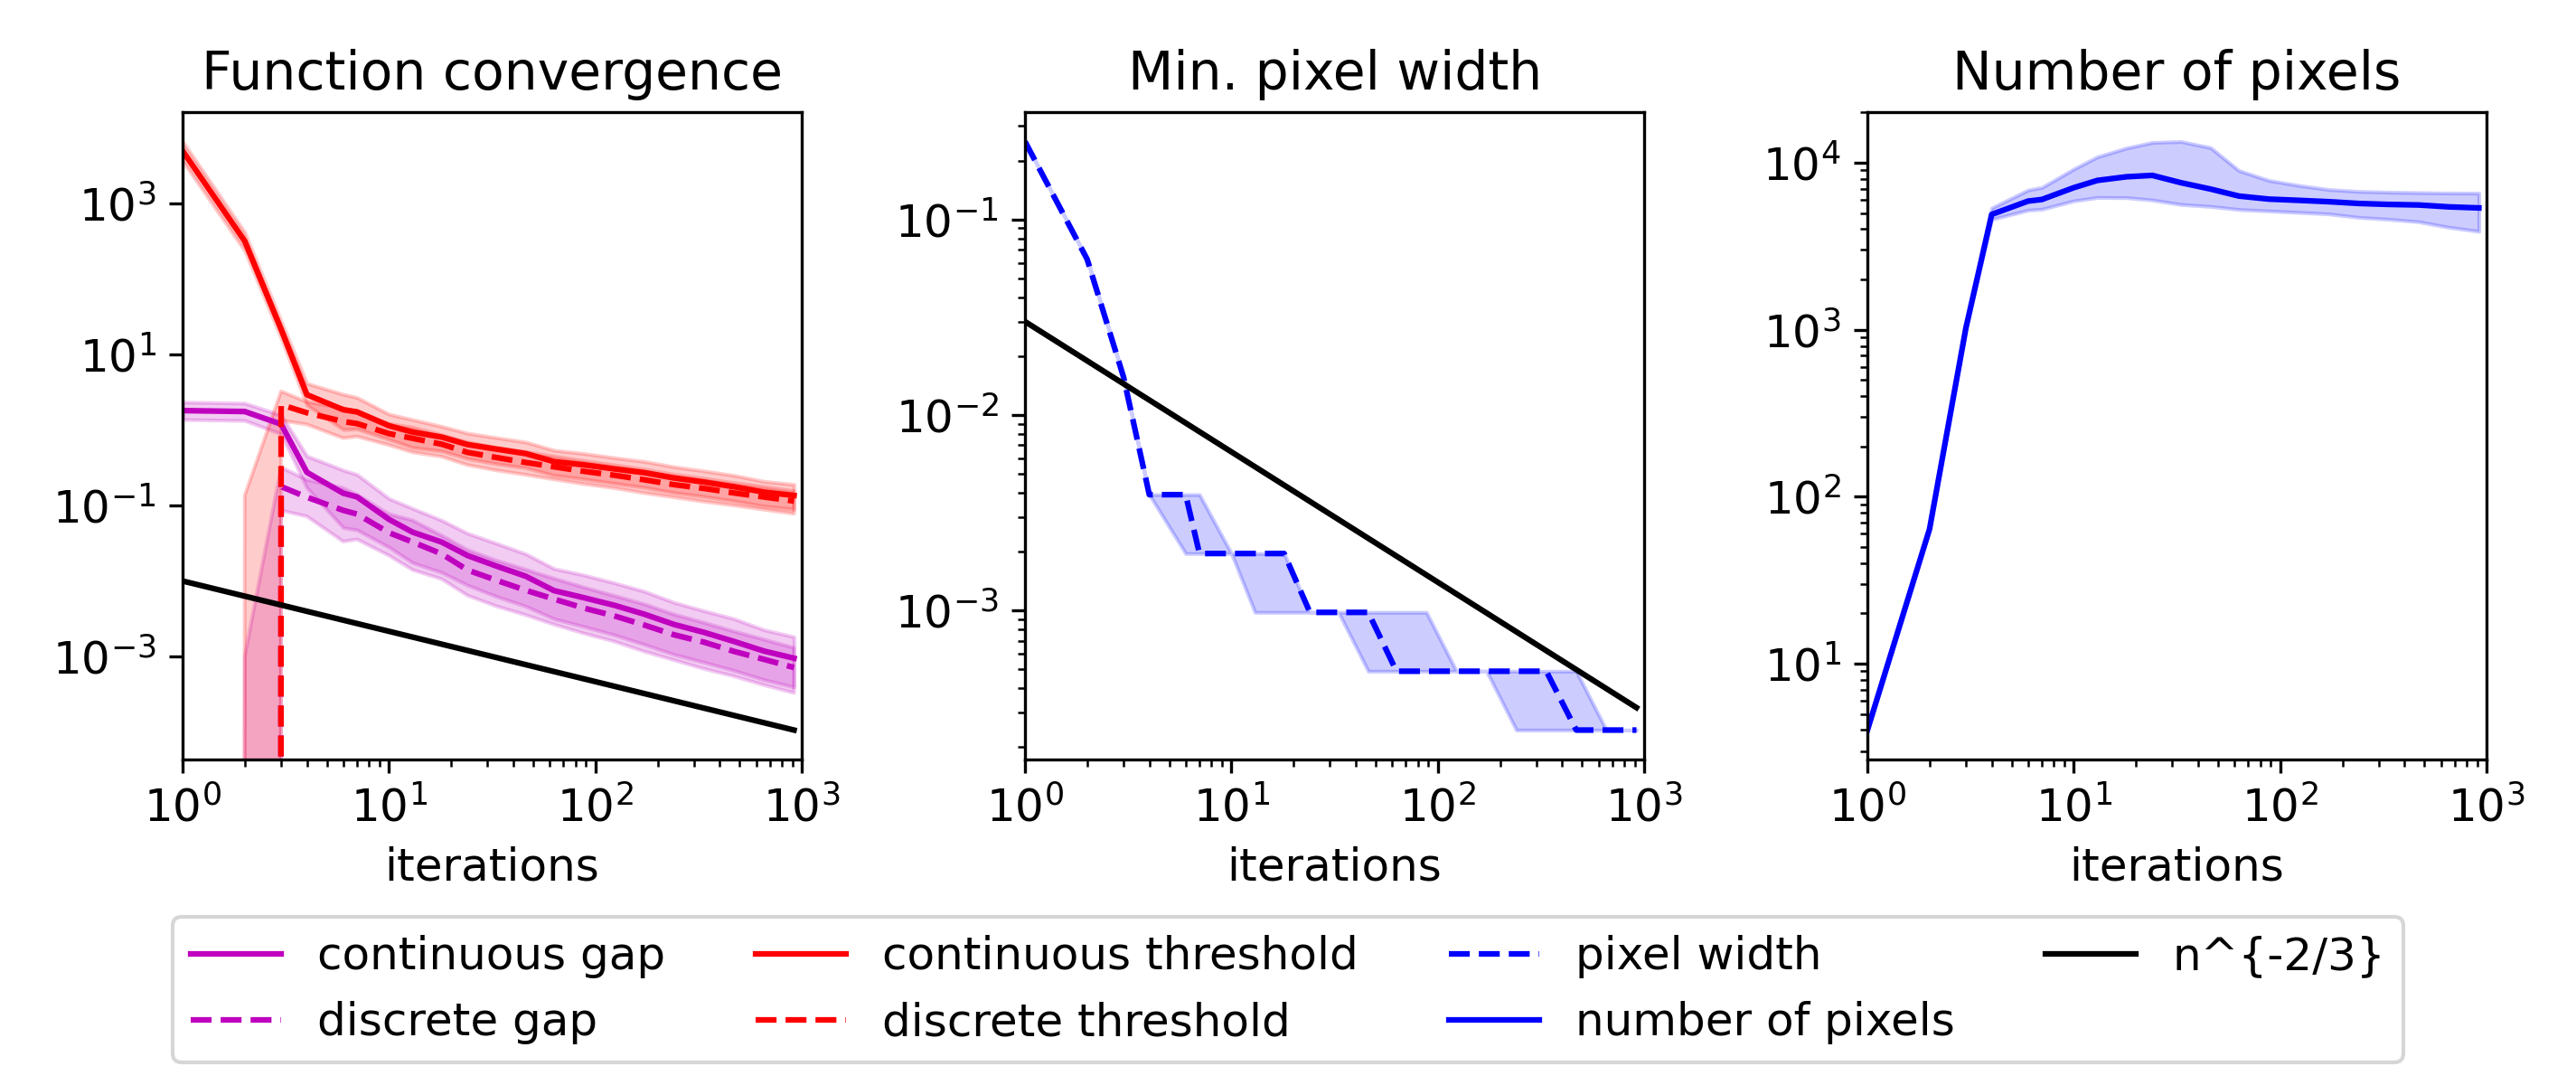
\includegraphics[width=\textwidth]{lasso2_convergence}
	\caption{Convergence of adaptive FISTA for STORM dataset. Lines indicate the median value over 3020 STORM frames. Shaded regions indicate the \SIrange{25}{75}{\percent} inter-quartile range.}\label{fig:ca: STORM convergence}
\end{figure}

\section{Conclusions and outlook}
In this work we have proposed a new adaptive variant of FISTA and provided convergence analysis. This algorithm allows FISTA to be applied outside of the classical Hilbert space setting, still with a guaranteed rate of convergence. We have presented several numerical examples where convergence with the refining discretisation is at least as fast as a uniform discretisation, although more efficient with regards to both memory and computation time. 

In 1D we see good agreement with the theoretical rate. This rate also seems to be a good predictor for all variants of FISTA tested, although this is yet to be proven. Surprisingly, even the classical methods with a fixed discretisation initially seem limited to the slower adaptive rate for small $n$.

The results in 2D are similar, all tested FISTA methods converge at least at the guaranteed rate. The wavelet example was most impressive, achieving nearly linear convergence in energy. This is similar to the behaviour for classical FISTA although it is also yet to be formally proven.

An interesting observation over all of the adaptive Lasso examples is that the classical oscillatory behaviour of FISTA has not occured. With the monotone gaps plotted, oscillatory convergence should correspond to a piecewise constant descending gap. Either this behaviour only emerges for larger $n$, or the adaptivity mimics the restarting behaviour typically used to avoid oscillation. The perturbation provided by the refinement is sufficient to stop FISTA overshooting the minimiser and maintain a predictable rate of convergence to the minimiser. This may also explain why the standard restarting FISTA showed little improvement in these examples.

Moving forward, it would be interesting to see how far the analysis extends to other optimisation algorithms. To cover the numerical results, this would necessitate repeating the presented argument for Forward-Backward splitting and for the modifications of FISTA suggested by \cite{Liang2018}. We feel that the extension to the primal-dual algorithm proposed by \cite{Chambolle2011} should also be possible where there is a classical bound of the form $\min_{n\leq N}\Func0(\varf0_n)+\Func0^*(\vvard0_n) \lesssim \frac{\norm{\varf0_0-\varf0^*}^2 + \norm{\vvard0_0-\vvard0^*}^2}{N}$. This has the same basic ingredients as FISTA although there is now the extra dual variable to account for.

Another interesting outlook is to relax the requirement for $\func1$ to be smooth on the whole of $\spcf0\cap\F H$. An example where this is not the case is the dual problem to total variation denoising where we have
$$ \Func0(\varf0) = \norm{\op{div}\varf0-\vdata0}^2 + \chi(\norm{\varf0}_\infty\leq \mu).$$
The divergence operator is not bounded in $L^2$ but is on each subspace $\spcf0^n$. It is not clear if it is possible to incorporate this into FISTA without restarting each time the step-size changes.

\bibliographystyle{apalike}\bibliography{references} % alpha is also a decent style
\newpage\appendix
\section{Proofs for FISTA convergence}\label{app:ca: FISTA convergence}
This section contains all of the statements and proofs of the results contained in \Cref{sec:ca: FISTA convergence}.

\subsection{Proofs for Step 2}

\begin{lemma}[\Cref{thm:ca: descent lemma}]\label{app:thm:ca: descent lemma}
	\Paste{thm:ca: descent lemma}
\end{lemma}
\begin{proof}
	This is exactly the result of \cite[Lemma 1]{Chambolle2015} applied to the function $\varf0\mapsto\Func0(\Pi_n\varf0)$.
\end{proof}



\begin{theorem*}[\Cref{thm:ca: one step FISTA}]
	\Paste{thm:ca: one step FISTA}
	\begin{equation}
		\vart1_{n}^2(\Func0(\varf0_{n}) - \Func0(\varf2_n)) - (\vart1_{n}^2-\vart1_{n})(\Func0(\varf0_{n-1})-\Func0(\varf2_n)) \leq \tfrac1{2}\left[\norm{\varf1_{n-1}}^2-\norm{\varf1_{n}}^2\right] + \IP{\varf1_{n}-\varf1_{n-1}}{\varf2_n}.\label{app:eq:ca: one-step FISTA}
	\end{equation}
\end{theorem*}
\begin{proof}
	Modifying \cite[Theorem 2]{Chambolle2015}, for $n\geq1$ we apply \Cref{app:thm:ca: descent lemma} with $\bar{\varf0} = \bar{\varf0}_{n-1}$ and $\varf2 = (1-\frac{1}{\vart1_{n}})\varf0_{n-1} + \frac{1}{\vart1_{n}}\varf2_n$. This gives
	$$\Func0(\varf0_{n}) + \tfrac12\norm{\tfrac{1}{\vart1_{n}}\varf1_{n}-\tfrac{1}{\vart1_{n}}\varf2_n}^2 \leq \Func0\left((1-\tfrac{1}{\vart1_{n}})\varf0_{n-1}+\tfrac{1}{\vart1_{n}}\varf2_n\right) + \tfrac12\norm{\tfrac{1}{\vart1_{n}}\varf1_{n-1}-\tfrac{1}{\vart1_{n}}\varf2_n}^2.$$
	By the convexity of $\Func0$, this reduces to
	\begin{align*}
		\Func0(\varf0_{n}) - \Func0(\varf2_n) - (1-\tfrac{1}{\vart1_{n}})[\Func0(\varf0_{n-1})-\Func0(\varf2_n)] &\leq \tfrac1{2\vart1_{n}^2}\norm{\varf1_{n-1}-\varf2_n}^2 - \tfrac1{2\vart1_{n}^2}\norm{\varf1_{n}-\varf2_n}^2
		\\ &= \tfrac1{2\vart1_{n}^2}\left[\norm{\varf1_{n-1}}^2-\norm{\varf1_{n}}^2\right] + \tfrac1{\vart1_{n}^2}\IP{\varf1_{n}-\varf1_{n-1}}{\varf2_n}.
	\end{align*}
\end{proof}



\begin{theorem}[\Cref{thm:ca: mini FISTA convergence}]\label{app:thm:ca: mini FISTA convergence}
	\Paste{thm:ca: mini FISTA convergence}
	\begin{multline}\label{app:eq:ca: FISTA inequality}
		\vart1_N^2\Func0_0(\varf0_N) + \sum_{n=1}^{N-1}\rho_n \Func0_0(\varf0_n) + \frac{\norm{\varf1_N-\varf2_N}^2}{2} \leq \frac{\norm{\varf0_0-\varf2_0}^2-\norm{\varf2_0}^2+\norm{\varf2_N}^2}{2}
		\\ + \sum^N_{n=1} \vart1_n\Func0_0(\varf2_n) + \IP{\varf1_{n-1}}{\varf2_{n-1}-\varf2_n}.
	\end{multline}
\end{theorem}
\begin{proof}
	\Cref{app:thm:ca: mini FISTA convergence} is just a summation of \eqref{app:eq:ca: one-step FISTA} over all $n=1,\ldots,N$. To see this: first add and subtract $\Func0(\varf0^*)$ to each term on the left-hand side to convert $\Func0$ to $\Func0_0$, then move $\Func0_0(\varf2_n)$ to the right-hand side. Now \eqref{app:eq:ca: one-step FISTA} becomes
	$$ \vart1_n^2\Func0_0(\varf0_n) - (\vart1_n^2-\vart1_n)\Func0_0(\varf0_{n-1}) \leq \vart1_n\Func0_0(\varf2_n) + \tfrac1{2}\left[\norm{\varf1_{n-1}}^2-\norm{\varf1_n}^2\right] + \IP{\varf1_n-\varf1_{n-1}}{\varf2_n}. $$
	Summing this inequality from $n=1$ to $n=N$ gives
	$$\vart1_N^2\Func0_0(\varf0_N) + \sum_{n=1}^{N-1}(\underbrace{\vart1_n^2-\vart1_{n+1}^2+\vart1_{n+1}}_{=\rho_n})\Func0_0(\varf0_n) \leq \frac{\norm{\varf1_0}^2-\norm{\varf1_N}^2}{2} + \sum_{n=1}^N \vart1_n\Func0_0(\varf2_n)+\IP{\varf1_n-\varf1_{n-1}}{\varf2_n}.$$
	This is almost in the desired form, however, we would like to flip the roles of $\varf1_n$/$\varf2_n$ in the final inner product term. Re-writing the right-hand side gives
	$$\sum_{n=1}^N\IP{\varf1_n-\varf1_{n-1}}{\varf2_n} = \IP{\varf1_N}{\varf2_N} - \IP{\varf1_0}{\varf2_0}+ \sum_{n=1}^N\IP{\varf1_{n-1}}{\varf2_{n-1}-\varf2_n}.$$
	Noting $\varf1_0=\varf0_0$, combining the previous two equations proves the statement of \Cref{app:thm:ca: mini FISTA convergence}.
\end{proof}



\newpage\noindent The following lemma is used to produce a sharper estimate on sequences $\vart1_n$.
\begin{lemma}\label{app:ca: tn upper bound}
	If $\rho_n=\vart1_{n}^2-\vart1_{n+1}^2+\vart1_{n+1}\geq0$, $\vart1_n\geq 1$ for all $n\in\F N$ then $\vart1_n\leq n-1 +\vart1_1$.
\end{lemma}
\begin{proof}
	This is trivially true for $n=1$. Suppose true for $n-1$, the condition on $\rho_{n-1}$ gives
	$$\vart1_n^2 -\vart1_n \leq \vart1_{n-1}^2 \leq (n-2+\vart1_1)^2 = (n-1+\vart1_1)^2 -2(n-1+\vart1_1) + 1.$$
	Assuming the contradiction, if $\vart1_n> n-1+\vart1_1$ then we get $n-1+\vart1_1 < 1$ but $\vart1_1\geq 1$ so this becomes $n<1$ which completes the contradiction.
\end{proof}



\begin{lemma}[\Cref{thm:ca: mini exponential FISTA convergence}]\label{app:thm:ca: mini exponential FISTA convergence}
	\Paste{thm:ca: mini exponential FISTA convergence}
\end{lemma}
\begin{proof}
	This is just a telescoping of the right-hand side of \eqref{app:eq:ca: FISTA inequality} with the introduction of $n_k$ and simplification $\varf2_n = \tilde{\varf2}_k$,
	\begin{multline*}
		\tfrac12\norm{\varf2_N}^2 + \sum^N_{n=1} \vart1_n\Func0_0(\Pi_n\varf2_n) + \IP{\varf1_{n-1}}{\varf2_{n-1}-\varf2_n} = \tfrac12\norm{\tilde{\varf2}_K}^2 + \sum_{n=n_K}^N\vart1_n\Func0_0(\tilde{\varf2}_K) 
		\\+ \sum_{k=1}^K\sum_{n=n_{k-1}}^{n_k-1}\vart1_n\Func0_0(\tilde{\varf2}_K) 
		+ \IP{\varf1_{n_k-1}}{\tilde{\varf2}_k-\tilde{\varf2}_{k+1}}.
	\end{multline*}
	\begin{samepage}
		By \Cref{app:ca: tn upper bound}, $\vart1_n\leq n$ so we can further simplify
		$$\sum_{n=\vars3}^{\vars4-1}\vart1_n \leq \sum_{n=\vars3}^{\vars4-1}n = (\vars4-\vars3)\frac{\vars4-1+\vars3}{2} \leq \frac{\vars4^2-\vars3^2}{2}$$
		to get the required bound.
	\end{samepage}
\end{proof}

\subsection{Proof for Step 3}
\begin{lemma}[\Cref{thm:ca: sufficiently fast}]\label{app:thm:ca: sufficiently fast}
	\Paste{thm:ca: sufficiently fast}
\end{lemma}
\todo{This proof is quite long and not very explicit. Should I compute the constant?}
\begin{proof}
	Inserting the assumed rates into \Cref{app:thm:ca: mini exponential FISTA convergence} gives
	$$	\vart1_N^2\Func0_0(\varf0_N) + \tfrac12\norm{\varf1_N-\tilde{\varf2}_K}^2 \lesssim \vars3_{\Varf0}^{2K} + (N+1)^2\vars3_{\Func0}^{-K} + \sum_{k=1}^{K}n_k^2\vars3_{\Func0}^{-k} + \vars3_{\Varf0}^{k}\norm{\varf1_{n_k-1}-\tilde{\varf2}_{k-1}} + \vars3_{\Varf0}^{2k}.$$
	Each case now needs its own induction. When $\vars3_{\Varf0}>1$ we simplify the inequality to 
	\begin{align*}
		\vart1_N^2\Func0_0(\varf0_N) + \tfrac12\norm{\varf1_N-\tilde{\varf2}_K}^2 &\lesssim \vars3_{\Varf0}^{2K} + \vars3_{\Varf0}^{2K+2} + \sum_{k=1}^{K}\vars3_{\Varf0}^{2k} + \vars3_{\Varf0}^{k}\norm{\varf1_{n_k-1}-\tilde{\varf2}_{k-1}}
		\\&\leq C_1\left(\vars3_{\Varf0}^{2K+2} + \frac{\vars3_{\Varf0}^{2K+2}}{\vars3_{\Varf0}^2-1} + \sum_{k=1}^{K}\vars3_{\Varf0}^{k}\norm{\varf1_{n_k-1}-\tilde{\varf2}_{k-1}}\right).
	\end{align*}
	for some $C_1$ sufficiently large. Assume $\norm{\varf1_{n_k-1}-\tilde{\varf2}_{k-1}}\leq C_2\vars3_{\Varf0}^k$ for $k\leq K$, then for $N=n_{K+1}-1$ we have
	$$\tfrac12\norm{\varf1_{n_{K+1}-1}-\tilde{\varf2}_K}^2 \leq \frac{C_1\vars3_{\Varf0}^{2K+2}}{\vars3_{\Varf0}^2-1}\left(\vars3_{\Varf0}^2+C_2\right).$$
	If $C_2$ is sufficiently large, then $\frac{C_1\vars3_{\Varf0}^{2K+2}}{\vars3_{\Varf0}^2-1}\left(\vars3_{\Varf0}^2+C_2\right) \leq \tfrac12C_2^2\vars3_{\Varf0}^{2K+2}$ which completes the induction. This bounds the growth of the right hand side and so for any $N<n_{K+1}$ we have $t_N^2\Func0_0(\varf0_N) \lesssim \vars3_{\Varf0}^{2K}$.
	
	When $\vars3_{\Varf0}=1$, the assumptions are stronger so the induction becomes more direct. Assuming $\norm{\varf1_{n_k-1}-\tilde{\varf2}_{k-1}}\leq C_2$ for $k\leq K$, there exists $C_1>0$ such that 
	\begin{align*}
		\vart1_{N+1}^2\Func0_0(\varf0_{N+1}) + \tfrac12\norm{\varf1_{N+1}-\tilde{\varf2}_{K}}^2 &\leq C_1 + \max_{k\leq K}\norm{\varf1_{n_k-1}-\tilde{\varf2}_{k-1}}
		\\&\leq C_1 + C_2.
	\end{align*}
	If $C_2$ is sufficiently large then $C_1 + C_2 \leq \tfrac14C_2^2$ which completes the second induction. This confirms $t_N^2\Func0_0(\varf0_N) \leq \tfrac14C_2^2$ is bounded uniformly.
\end{proof}

\subsection{Proof for Step 4}
\begin{lemma}[\Cref{thm:ca: sufficiently slow}]\label{app:thm:ca: sufficiently slow}
	\Paste{thm:ca: sufficiently slow}
\end{lemma}
\begin{proof}
	The proof is direct computation,
	$$ \log N^2 \geq \log C + K\left(\log \vars3_{\Func0} + \log \vars3_{\Varf0}^2\right)$$ 
	which leads to
	\begin{align*}
		\vars3_{\Varf0}^{2K} & = \exp(K\log \vars3_{\Varf0}^2)
		\\&\leq \exp\left(\log N^2\frac{\log \vars3_{\Varf0}^2}{\log \vars3_{\Func0} + \log \vars3_{\Varf0}^2} - \frac{\log C\log \vars3_{\Varf0}^2}{\log \vars3_{\Func0} + \log \vars3_{\Varf0}^2}\right)
		\\&\lesssim N^{2\epsilon}
	\end{align*}
	as required.
\end{proof}



\begin{theorem}[\Cref{thm:ca: exponential FISTA convergence}]
	\Paste{thm:ca: exponential FISTA convergence}
\end{theorem}
\begin{proof}
	If the conditions of this theorem are satisfied, then so are \Cref{app:thm:ca: mini exponential FISTA convergence,app:thm:ca: sufficiently fast,app:thm:ca: sufficiently slow}. The final result is just the conclusion of \Cref{app:thm:ca: sufficiently slow}.
\end{proof}


\subsection{Proofs for Step 5}
\begin{theorem}[\Cref{thm:ca: stronger exponential FISTA convergence}]\label{app:thm:ca: stronger exponential FISTA convergence}
	\Paste{thm:ca: stronger exponential FISTA convergence}
\end{theorem}
\begin{proof}
	To apply \Cref{app:thm:ca: sufficiently fast}, we need
	$$n_k^2\lesssim \splitln{(\vars3_{\Func0}\vars3_{\Varf0}^2)^k}{\vars3_{\Varf0}>1}{k^{-2}\vars3_{\Func0}^k}{\vars3_{\Varf0}=1}, \qquad \norm{\tilde{\varf2}_k}\lesssim \vars3_{\Varf0}^{k}, \qquad \text{ and } \Func0_0(\tilde{\varf2}_k)\lesssim \vars3_{\Func0}^{-k}$$
	and $\sum_{k=1}^\infty\norm{\tilde{\varf2}_k-\tilde{\varf2}_{k+1}}<\infty$ when $\vars3_{\Varf0}=1$. The only one which is not directly assumed is easily verified,
	$$\Func0_0(\tilde{\varf2}_k) = \min_{\varf0\in\spcf0^{n_k}}\Func0_0(\varf0) \leq\Func0_0(\varf0_{n_k-1}) \lesssim \vars3_{\Func0}^{-k}.$$
	Therefore, the result of \Cref{app:thm:ca: sufficiently fast} gives
	$$\Func0_0(\varf0_N) \lesssim \frac{\vars3_{\Varf0}^{2K}}{\vart1_N^2} \lesssim \frac{\vars3_{\Varf0}^{2K}}{N^2}.$$
	In the case $\vars3_{\Varf0}=1$, this is already the optimal rate and therefore sharp. If this were sharp for general $\vars3_{\Varf0}$ and $\Func0$, then we gain nothing by refining early (increasing $K$ for fixed $N$) however, we can at least guarantee that refining early does not lose the optimal rate.
	
	\begin{samepage}
		If we fix $N^2\lesssim (\vars3_{\Func0}\vars3_{\Varf0}^2)^k$, then
		$$\min_{n\leq N} \Func0_0(\varf0_n)\lesssim \splitln{\vars3_{\Func0}^{-k}}{N>n_k}{ \sfrac{\vars3_{\Varf0}^{2k}}{N^2}}{N\leq n_k} \lesssim N^{-2}\max(\vars3_{\Varf0}^{2k},\vars3_{\Varf0}^{2k}) \lesssim N^{-2(1-\epsilon)}$$
		as required.
	\end{samepage}
\end{proof}



\begin{lemma}[\Cref{thm:ca: practical refinement criteria}]
	\Paste{thm:ca: practical refinement criteria}
\end{lemma}
\todo{This is a very long theorem which I don't really use in the end. The result is a little bit useful but not difficult.}
\begin{proof}
	The proof is simply to justify that the conditions of \Cref{app:thm:ca: stronger exponential FISTA convergence} are met for all refinement criteria described here. $\norm{\tilde{\varf2}_k}\lesssim \vars3_{\Varf0}^k$ is enforced at every step and condition (2) guarantees the back-stop condition on $n_k$.
	
	To complete the requirements of \Cref{app:thm:ca: stronger exponential FISTA convergence}, we first need to show inductively that $\Func0_0(\tilde{\varf2}_{k-1}) \leq C\vars3_{\Func0}^{-k}$, then it follows that $\Func0_0(\varf0_{n_k-1})\leq C\vars3_{\Func0}^{-k}$. To be explicit, when $\Func0$ has bounded sublevel sets, assume that the bound for $\{\varf0\in\F H\st \Func0(\varf0)\leq \Func0(\varf0_0)\}$ is $R>0$.
	
	For (2) and (5) the decay of $\Func0_0(\tilde{\varf2}_{k-1})$ is already assumed but otherwise we need to perform the formal induction. Assume $\Func0_0(\tilde{\varf2}_{k-1}) \leq C\vars3_{\Func0}^{1-k}$, then for each remaining adaptive criterion:
	\begin{itemize}
		\item[(1)] $\Func0_0(\tilde{\varf2}_k)\leq \Func0_0(\varf0_{k})\leq\vars1 \vars3_{\Func0}^{-k}$ by definition, the induction holds if $C\geq \vars1$.
		\item[(3)] $\Func0_0(\tilde{\varf2}_k)\leq \Func0_0(\varf0_{k})\leq\frac{\vars1}{1-\vars1}\Func0_0(\tilde{\varf2}_{k-1})$, the induction holds if $\vars1\leq \frac{1}{1+\vars3_{\Func0}}$.
		\item[(4)] $\Func0_0(\tilde{\varf2}_k)\leq \Func0_0(\varf0_{k}) \leq \IP{\partial\Func0(\varf0_{k})}{\varf0_{n_k-1}-\varf0^*} \leq 2R\vars1\vars3_{\Func0}^{-k}$, the induction holds for $C\geq 2R\vars1$.
	\end{itemize}
	In each case, with $C$ sufficiently large, the induction holds. Now we can return to the precise condition of \Cref{app:thm:ca: stronger exponential FISTA convergence}, $\Func0_0(\varf0_{n_k-1}) \leq C'\vars3_{\Func0}^{-k}$. Assume true for $k-1$. For each adaptive criterion:
	\begin{itemize}
		\item[(1)] $\Func0_0(\varf0_{k})\leq\vars1 \vars3_{\Func0}^{-k}$ is by definition.
		\item[(2)] $\Func0_0(\varf0_{k})\leq\vars1 \vars3_{\Func0}^{-k} + \Func0_0(\tilde{\varf2}_{k-1})$ requires $C'\geq \vars1+\vars3_{\Func0}C$.
		\item[(3)] $\Func0_0(\varf0_{k})\leq\frac{\vars1}{1-\vars1}\Func0_0(\tilde{\varf2}_{k-1})$ requires $C'\geq \frac{\vars1}{1-\vars1}C$.
		\item[(4)] $\Func0_0(\varf0_{k}) \leq 2R\vars1\vars3_{\Func0}^{-k}$, the induction holds for large $C'$.
		\item[(5)] $\Func0_0(\varf0_{k})\leq 2R\vars1\vars3_{\Func0}^{-k} + \Func0_0(\tilde{\varf2}_{k-1})$, the induction holds for large $C'\geq 2R\vars1+C$.
	\end{itemize}
	This completes the requirements of \Cref{app:thm:ca: stronger exponential FISTA convergence}, therefore also this proof.
\end{proof}


\section{Proof of \texorpdfstring{\Cref{thm:ca: generic a_U and a_E}}{rates for general finite element spaces}}\label{app:ca: generic a_U and a_E}
\todo{This whole section is unnecessary for the numerics. It is possibly useful to get a general understanding of the rates one can achieve but not strong enough for Lasso. It is quite a long proof for that level of reward\ldots}
The proof of \Cref{thm:ca: generic a_U and a_E} is the result of the following three lemmas. The first, \Cref{app:thm:ca: generic a_U bound}, is a general quantification of the equivalence between $L^q$ and $L^2$ norms on finite dimensional sub-spaces. A special case occurs when $q=1$ because the dual norm is a supremum rather than an integral. In \Cref{app:thm:ca: specific a_U bound}, this locality is exploited by finite element spaces, which we assumed had a basis with local support. \Cref{app:thm:ca: generic a_E bound} then performs the computations for the $\vars3_{\Func0}$ constant depending on the smoothness properties of $\Func0$.

\begin{lemma}\label{app:thm:ca: generic a_U bound}
	Suppose $\F H= L^2(\Domain)$ for some compact domain $\Domain\subset\R^d$ and $\norm\cdot_q\lesssim \Norm\cdot$ for some $q\in[1,\infty]$. Let $\tilde{\spcf0}\subset \spcf0\cap\F H$ be a finite dimensional subspace with orthonormal basis $\{e_j\st j=1,\ldots,\op{dim}(\tilde{\spcf0})\}\subset\tilde{\spcf0}$ and orthogonal projection $\Pi\colon\F H\to\tilde{\spcf0}$. If these conditions hold, then:
	\begin{itemize}
		\item if $q\geq 2$, then $$\norm{\Pi\varf2} \lesssim \Norm{\varf2}, $$
		\item otherwise, if $e_j\in \spcf0^*$, then
		$$\norm{\Pi\varf2} \leq \sqrt{\op{dim}(\tilde{\spcf0})}\max_j\Norm{e_j}_*\Norm{\varf2},$$
		\item otherwise, if $e_j\in L^\infty(\Domain)$ and $ |\{j:e_j(\vvarx0)\neq 0\}|\leq C$ for almost all $\vvarx0\in\Domain$, then
		$$\norm{\Pi\varf2} \lesssim \sqrt C\max_j\norm{e_j}_{L^\infty}\Norm{\varf2} $$
	\end{itemize}
	uniformly for all $\varf2\in \F H$.
\end{lemma}
\begin{proof}
	The first statement for $q\geq 2$ is from H\"older's inequality combined with the fact that compact domains have finite volume,
	$$\norm{\Pi\varf2}^2 \leq \norm{\varf2}^2 = \norm{\varf2}_2^2 = \norm{\varf2^2}_1 \lesssim \norm{\varf2}_q^2 \lesssim \Norm{\varf2}^2.$$
	The remaining statements come from the equivalence of norms on finite dimensional spaces. Note that
	$$\norm{\Pi\varf2} = \frac{\IP{\Pi\varf2}{\Pi\varf2}}{\norm{\Pi\varf2}} = \frac{\IP{\Pi\varf2}{\varf2}}{\norm{\Pi\varf2}} \leq \frac{\Norm{\Pi\varf2}_*}{\norm{\Pi\varf2}}\Norm{\varf2},$$
	therefore it is sufficient to bound $\frac{\Norm\cdot_*}{\norm\cdot}$ on the subspace $\tilde{\spcf0}$. Switching to the given basis, for $\varf0 = \sum_j \varx3_je_j$ we have
	\begin{align*}
		\norm{\varf0}^2 &= \sum_{j=1}^{\op{dim}(\tilde{\spcf0})} \varx3_j^2 = \norm{\vvarx3}_{\ell^2}^2,
		\\\Norm{\varf0}_*&\leq \sum_{j=1}^{\op{dim}(\tilde{\spcf0})} |\varx3_j|\Norm{e_j}_* \leq \max_j\Norm{e_j}_*\norm{\vvarx3}_{\ell^1},
		\\\implies \frac{\Norm{\varf0}_*}{\norm{\varf0}} &\leq \max_j\Norm{e_j}_*\frac{\norm{\vvarx3}_{\ell^1}}{\norm{\vvarx3}_{\ell^2}} \leq \max_j\Norm{e_j}_*\sqrt{\op{dim}(\tilde{\spcf0})}.
	\end{align*}
	Alternatively, we can use the inequality
	$$\norm{\Pi\varf2} = \frac{\IP{\Pi\varf2}{\varf2}}{\norm{\Pi\varf2}} \leq \frac{\norm{\Pi\varf2}_{\infty}}{\norm{\Pi\varf2}}\norm{\varf2}_1\lesssim  \frac{\norm{\Pi\varf2}_{\infty}}{\norm{\Pi\varf2}}\norm{\varf2}_q \lesssim \frac{\norm{\Pi\varf2}_{\infty}}{\norm{\Pi\varf2}}\Norm{\varf2}.$$
	This simplifies the equivalence constant because for any $\varf0 = \sum \varx3_je_j$ and $\mu>1$, there exists a set of points $\vvarx0\in\Domain$ with non-zero measure such that $\norm{\varf0}_\infty\leq \mu|\varf0(\vvarx0)|$. This gives
	\begin{align*}
		\norm{\varf0}^2 &= \sum \varx3_j^2 \geq \sum_{e_j(\vvarx0)\neq 0} \varx3_j^2,
		\\\norm{\varf0}_\infty& \leq \mu|\varf0(\vvarx0)| \leq \mu\sum_{e_j(\vvarx0)\neq 0} |\varx3_j|\norm{e_j}_\infty,
		\\\implies \frac{\norm{\varf0}_\infty}{\norm{\varf0}} &\leq \mu\max_j\norm{e_j}_\infty\sqrt{C}.
	\end{align*}
	This inequality holds for all $\mu>1$ therefore also for $\mu=1$. Essentially, with an extra smoothness assumption on $e_j$, we can reduce the dimension of the problem to $\op{dim}(\tilde{\spcf0})=C $ and use the previous result.
\end{proof}



\begin{lemma}\label{app:thm:ca: specific a_U bound}
	Suppose $\F H= L^2(\Domain)$ for some compact domain $\Domain\subset\R^d$ and $\norm\cdot_q\lesssim \Norm\cdot$ for some $q\in[1,\infty]$. Let $(\tilde{\spcf0}^k)_k$ be a sequence of $\meshsize$-refining finite element spaces with orthogonal projections $\tilde\Pi_k\colon\F H\to\tilde{\spcf0}^k $. If $q\geq 2$,
	$$\norm{\tilde\Pi_k\varf2} \lesssim \Norm{\varf2}, $$
	otherwise,
	$$\norm{\tilde\Pi_k\varf2} \lesssim \sqrt{\op{dim}(\tilde{\spcf0}^0)}\meshsize^{-\frac{kd}{2}}\Norm{\varf2} $$
	uniformly for all $\varf2\in \F H$.
\end{lemma}
\begin{proof}
	Most of the conditions of \Cref{app:thm:ca: generic a_U bound} are already satisfied. Denote $C=\op{dim}(\tilde{\spcf0^0})$ and $\{e_j\st j\in[C]\}$ the standard orthonormal basis of $\tilde{\spcf0}^0$. The scaling properties of $\meshsize$-refining finite element spaces guarantee that the value of $C$ satisfies the conditions of \Cref{app:thm:ca: generic a_U bound} and a basis of $\tilde{\spcf0}^k$ is given by
	$$ \left\{\vvarx0\mapsto\varf0_j(\vars0^{i,k}\vvarx0+\vvars1^{i,k}) \qquad\st\qquad i=1,\ldots,|\F M^k|,\ j=1,\ldots,C\right\}$$
	for some $\vars0^{i,k}\in\R^{d\times d}$, and $\vvars1^{i,k}\in\R^d$ such that $0<\op{det}(\vars0^{i,k})\lesssim \meshsize^{-kd}$.
	
	We now compute the scaling constant in \Cref{app:thm:ca: generic a_U bound}:
	$$ \frac{\norm{\varf0_j(\vars0^{i,k}\cdot+\vvars1^{i,k})}_\infty}{\norm{\varf0_j(\vars0^{i,k}\cdot+\vvars1^{i,k})}} = \frac{\norm{\varf0_j}_\infty}{\sqrt{\int_{\domain_i^k} e_j(\vars0^{i,k} \vvarx0+\vvars1^{i,k})^2d\vvarx0}} = \frac{\norm{\varf0_j}_\infty}{\sqrt{\op{det}(\vars0^{i,k})^{-1}}} \lesssim \meshsize^{-\frac{kd}{2}}.$$
	This value is independent of $j$ and gives the desired bound as a result of \Cref{app:thm:ca: generic a_U bound}.
\end{proof}



\begin{lemma}\label{app:thm:ca: generic a_E bound}
	Let $(\tilde{\spcf0}^k)_k$ be a sequence of $\meshsize$-refining finite element spaces of order $p$ with $\tilde{\varf2}^k=\argmin_{\varf0\in\tilde{\spcf0}^k}\Func0(\varf0)$.
	\begin{enumerate}
		\item If $\Func0$ is $\Norm\cdot$-Lipschitz at $\varf0^*$, then
		$\Func0(\tilde{\varf2}^k)-\Func0(\varf0^*) \lesssim \meshsize^p\Norm{\varf0^*}.$
		\item If $\Func0$ is $\Norm\cdot$-smooth at $\varf0^*$, then 
		$\Func0(\tilde{\varf2}^k)-\Func0(\varf0^*) \lesssim \meshsize^{2p}\Norm{\varf0^*}.$
		\item If $\func1$ is $\Norm\cdot$-Lipschitz at $\varf0^*$ and 
		$$\min_{\varf2\in\tilde{\spcf0}^k}\left\{\Norm{\varf2-\varf0^*}\st \func2(\varf2)\leq \func2(\varf0^*)\right\} \lesssim \min_{\varf2\in\tilde{\spcf0}^k}\Norm{\varf2-\varf0^*}$$
		uniformly for $k\in\F N$, then
		$\Func0(\tilde{\varf2}^k)-\Func0(\varf0^*) \lesssim \meshsize^p\Norm{\varf0^*}.$
	\end{enumerate}
\end{lemma}
\begin{proof}
	Each statement is by definition, observe
	\begin{gather*}
		\Func0(\varf2)-\Func0(\varf0^*) \leq \op{Lip}(\Func0)\Norm{\varf2-\varf0^*},
		\\\Func0(\varf2)-\Func0(\varf0^*) \leq \IP{\partial \Func0(\varf2)}{(\varf2-\varf0^*)} = \IP{\nabla \Func0(\varf2)-\nabla \Func0(\varf0^*)}{ \varf2-\varf0^*} \leq \op{Lip}(\nabla F)\Norm{\varf2-\varf0^*}^2,
		\\\Func0(\varf2)-\Func0(\varf0^*) \leq \func1(\varf2)-\func1(\varf0^*) \leq \op{Lip}(\func1)\Norm{\varf2-\varf0^*}.
	\end{gather*}
	Minimising over the right-hand side over $\varf2$ and substituting the definition of order gives the desired result.
\end{proof}


\section{Operator norms for numerical examples}
\begin{theorem}[\Cref{thm:ca: norm bound examples}]\label{app:thm:ca: norm bound examples}
	\Paste{thm:ca: norm bound examples}
\end{theorem}
\todo{A very boring theorem but needs to be somewhere to justify the numerics. I don't know if the $\Delta\ll\sigma$ case is interesting to anyone else.}
\begin{proof}[Proof case 1:]
	From \Cref{thm:ca: norm bound L2} we have 
	$$(\A\A^*)_{i,j} = \IP{\1_{\F{\Varx0}_i}}{\1_{\F{\Varx0}_j}} = |\F{\Varx0}_i\cap \F{\Varx0}_j| = \splitln{|\F{\Varx0}_i|}{i=j}{0}{i\neq j}.$$
	Therefore, $\A\A^*$ is a diagonal matrix and $\norm{\A\A^*}_{\ell^2\to\ell^2} = \max_j |\F{\Varx0}_j|$ completes the result.
\end{proof}

\begin{proof}[Proof case 2:]
	$\vard1_j$ are not necessarily orthogonal however $|\IP{\vard1_i}{\vard1_j}|\leq 1$ therefore we can estimate
	$$\norm{\A\A^*}_{\ell^2\to\ell^2} \leq \norm{\A\A^*}_{\ell^\infty\to\ell^\infty} \leq m.$$
	Now looking to apply \Cref{thm:ca: norm bound smoothness}, note $\norm{\nabla^k\vard1_j}_\infty \leq \Vars3^k$, therefore
	\begin{align*}
		|\A^*\vvarx3|_{C^k}&\leq \Vars3^k m^{\frac1{q^*}}\norm{\vvarx3}_q = \Vars3^k m^{1-\frac1{q}}\norm{\vvarx3}_q,
		\\|\A^*|_{\ell^2\to C^k} &\leq \Vars3^k \min_{q\in[1,\infty]}m^{1-\frac1q}\sqrt{m}^{\max(0,2-q)} = \sqrt{m}\Vars3^k.
	\end{align*}
\end{proof}

\begin{proof}[Proof of asymptotic case 3:]
	In the Gaussian case, we build our approximations around the idea that sums of Gaussians on a regular grid look like a discretised integral. The first example can be used to approximate the operator norm. Computing the inner products gives
	\\\parbox{\linewidth+5pt}{\begin{multline*}
				\IP{\vard1_i}{\vard1_j} = (2\pi\sigma^2)^{-d}\int_{[0,1]^d} \exp\left(-\tfrac{|\vvarx0-\vvarx0_i|^2}{2\sigma^2}-\tfrac{|\vvarx0-\vvarx0_j|^2}{2\sigma^2}\right) \leq (2\pi\sigma^2)^{-d}(\pi\sigma^2)^{\frac{d}{2}}\exp\left(-\tfrac{|\vvarx0_i-\vvarx0_j|^2}{4\sigma^2}\right) 
				\\= (4\pi\sigma^2)^{-\frac d2} \exp\left(-\tfrac{|\vvarx0_i-\vvarx0_j|^2}{4\sigma^2}\right).
	\end{multline*}}
	Estimating the operator norm,
	\\{\centering\resizebox{.9\textwidth}{!}{\parbox{\textwidth}{\begin{align*}
					\norm{\A\A^*}_{\ell^2\to\ell^2}&\leq \norm{\A\A^*}_{\ell^\infty\to\ell^\infty} = \max_{i\in[m]} \sum_{j=1}^m |\IP{\vard1_i}{\vard1_j}| 
					\\&= \max_{i\in[m]}(4\pi\sigma^2)^{-\frac d2}\sum_{j_1,\ldots,j_d\in[\hat m]} \exp\left(-\frac{(j_1\Delta-i_1\Delta)^2+\ldots+(j_d\Delta-i_d\Delta)^2}{4\sigma^2}\right)
					\\&\leq (4\pi\sigma^2)^{-\frac d2}\sum_{\vec j\in\F Z^d\cap[-\hat m,\hat m]^d} \exp\left(-\frac{(j_1\Delta)^2+\ldots+(j_d\Delta)^2}{4\sigma^2}\right)
					\\&= \frac{(4\pi)^{-\frac d2}}{\Delta^d}\sum_{\vec j\in\F Z^d\cap[-\hat m,\hat m]^d} \exp\left(-\frac14\left|\vec j\frac{\Delta}{\sigma}\right|^2\right)\frac{\Delta^d}{\sigma^d}
					\\&\sim \frac{(4\pi\sigma^2)^{-\frac d2}}{\Delta^d}\int_{\R^d} \exp\left(-\tfrac{|\vvarx0|^2}{4\sigma^2}\right) \quad = \Delta^{-d}.
	\end{align*}}}}
	\\This is a nice approximation because it depends only on $\Delta$, overcoming the $\frac1\sigma$ scaling. To convert this into an upper bound, we just compute the sum explicitly. In particular, as the sum factorises over dimensions,
	$$\norm{\A\A^*}_{\ell^2\to\ell^2} \leq (4\pi\sigma^2)^{-\frac d2}\left(\sum_{j=-\hat m,\ldots, \hat m}\exp\left(-\tfrac{\Delta^2}{4\sigma^2}j^2\right)\right)^d.$$
	Applying the same ideas to \Cref{thm:ca: norm bound smoothness}, note
	$$\begin{array}{rll}
			\displaystyle |\vard1_j(\vvarx0)| &\displaystyle= \left|\vard1_j(\vvarx0)\right| &\displaystyle = (2\pi\sigma^2)^{-\frac d2}\exp\left(-\frac{|\vvarx0-\vvarx0_j|^2}{2\sigma^2}\right),
			\\\displaystyle |\nabla\vard1_j(\vvarx0)| &\displaystyle= \left|\frac{\vvarx0-\vvarx0_j}{\sigma^2}\vard1_j(\vvarx0)\right| &\displaystyle = \frac{(2\pi\sigma^2)^{-\frac d2}}{\sigma}\frac{|\vvarx0-\vvarx0_j|}{\sigma}\exp\left(-\frac{|\vvarx0-\vvarx0_j|^2}{2\sigma^2}\right),
			\\|\nabla^2\vard1_j(\vvarx0)| &\displaystyle =\left|\frac1{\sigma^2} + \frac{(\vvarx0-\vvarx0_j)(\vvarx0-\vvarx0_j)^\top }{\sigma^4}\right|\vard1_j(\vvarx0) &\displaystyle = \frac{(2\pi\sigma^2)^{-\frac d2}}{\sigma^2}\left(1+\frac{|\vvarx0-\vvarx0_j|^2}{\sigma^2}\right)\exp\left(-\frac{|\vvarx0-\vvarx0_j|^2}{2\sigma^2}\right).
	\end{array}$$
	With the substitution $\vvarx0=\frac{\Delta}{\sigma}\vec j$, the asymptotic bounds on these are clear:
	\begin{align*}
		\sum_{\vec j\in[\hat m]^d} |\vard1_{\vec j}(\vvarx0)|^{q^*} &\lesssim (2\pi\sigma^2)^{-\frac{dq^*}{2}}\frac{\sigma^d}{\Delta^d}\int_{\R^d}\exp\left(-\frac{q^*|\vvarx0|^2}{2}\right),
		\\\sum_{\vec j\in[\hat m]^d} |\nabla\vard1_{\vec j}(\vvarx0)|^{q^*} &\lesssim \frac{(2\pi\sigma^2)^{-\frac{dq^*}{2}}}{\sigma}\frac{\sigma^d}{\Delta^d}\int_{\R^d}|\vvarx0|^{q^*}\exp\left(-\frac{q^*|\vvarx0|^2}{2}\right),
		\\\sum_{\vec j\in[\hat m]^d} |\nabla^2\vard1_{\vec j}(\vvarx0)|^{q^*} &\lesssim \frac{(2\pi\sigma^2)^{-\frac{dq^*}{2}}}{\sigma^2}\frac{\sigma^d}{\Delta^d}\int_{\R^d}(1+|\vvarx0|^2)^{q^*}\exp\left(-\frac{q^*|\vvarx0|^2}{2}\right).
	\end{align*}
\end{proof}

\begin{proof}[Proof of precise case 3:]
	In the asymptotic case we have shown
	$$\begin{array}{rll}
			\displaystyle |\vard1_j(\vvarx0)| &\displaystyle= \left|\vard1_j(\vvarx0)\right| &\displaystyle = (2\pi\sigma^2)^{-\frac d2}\exp\left(-\frac{|\vvarx0-\vvarx0_j|^2}{2\sigma^2}\right),
			\\\displaystyle |\nabla\vard1_j(\vvarx0)| &\displaystyle= \left|\frac{\vvarx0-\vvarx0_j}{\sigma^2}\vard1_j(\vvarx0)\right| &\displaystyle = \frac{(2\pi\sigma^2)^{-\frac d2}}{\sigma}\frac{|\vvarx0-\vvarx0_j|}{\sigma}\exp\left(-\frac{|\vvarx0-\vvarx0_j|^2}{2\sigma^2}\right),
			\\|\nabla^2\vard1_j(\vvarx0)| &\displaystyle =\left|\frac1{\sigma^2} + \frac{(\vvarx0-\vvarx0_j)(\vvarx0-\vvarx0_j)^\top }{\sigma^4}\right|\vard1_j(\vvarx0) &\displaystyle = \frac{(2\pi\sigma^2)^{-\frac d2}}{\sigma^2}\left(1+\frac{|\vvarx0-\vvarx0_j|^2}{\sigma^2}\right)\exp\left(-\frac{|\vvarx0-\vvarx0_j|^2}{2\sigma^2}\right).
	\end{array}$$
	We now wish to sum over $j=1,\ldots,m$ and produce an upper bound on these, independent of $t$. To do so we will use the following lemma.
	
	\begin{lemma}\label{app:ca: exp sum bound}
		Suppose $q>0$. If the polynomial $p(|\vvarx0|) = \sum p_k|\vvarx0|^k$ has non-negative coefficients and $\vvarx0\in[-m,m]^d$, then
		$$\sum_{\substack{\vec{j}\in\F Z^d\\\norm{\vec{j}}_{\ell^\infty}\leq m}} p(|\vec{j}-\vvarx0|)\exp\left(-\tfrac{q|\vec{j}-\vvarx0|^2}{2}\right)\leq \left[\sum_{\substack{\vec{j}\in\F Z^d\\\norm{\vec{j}}_{\ell^\infty}\leq2m}}p(|\vec{j}|+\delta)\exp\left(-\frac{q\max(0,|\vec{j}|-\delta)^2}{2}\right)\right]$$
		where $\delta\coloneqq \frac{\sqrt{d}}{2}$.
	\end{lemma}
	\begin{proof}
		There exists $\hat{\vvarx0}\in[-\tfrac12,\tfrac12]^d$ such that $\vvarx0 + \hat{\vvarx0}\in\F Z^d$, therefore
		\begin{align*}
			\sum_{\substack{\vec{j}\in\F Z^d\\\norm{\vec{j}}_{\ell^\infty}\leq m}} p(|\vec{j}-\vvarx0|)\exp\left(-\tfrac{q|\vec{j}-\vvarx0|^2}{2}\right) &= \sum_{\substack{\vec{j}\in\F Z^d\\\norm{\vec{j}}_{\ell^\infty}\leq m}} p(|\vec{j}-(\vvarx0+\hat{\vvarx0})+\hat{\vvarx0}|)\exp\left(-\tfrac{q|\vec{j}-(\vvarx0+\hat{\vvarx0})+\hat{\vvarx0}|^2}{2}\right)
			\\&\leq \sum_{\substack{\vec{j}\in\F Z^d\\\norm{\vec{j}}_{\ell^\infty}\leq2m}} p(|\vec{j}+\hat{\vvarx0}|)\exp\left(-\tfrac{q|\vec{j}+\hat{\vvarx0}|^2}{2}\right)
			\\&\leq \sum_{\substack{\vec{j}\in\F Z^d\\\norm{\vec{j}}_{\ell^\infty}\leq2m}} p(|\vec{j}|+\delta)\exp\left(-\tfrac{q\max(0,|\vec{j}|-\delta)^2}{2}\right)
		\end{align*}
		as $|\hat{\vvarx0}|\leq \delta$ and $p$ has non-negative coefficients. 
	\end{proof}
	
	Now, continuing the proof of \Cref{app:thm:ca: norm bound examples}, for $\hat m=\sqrt[d]{m}$, $\delta=\frac{\sqrt{d}}{2}$ and $J=\{\vec{j}\in\F Z^d \st \norm{\vec{j}}_{\ell^\infty}\leq 2\hat m\}$, \Cref{app:ca: exp sum bound} bounds 
	\begin{align*}
		\sum_{j=1}^m |\vard1_j(\vvarx0)|^{q^*} &\leq (2\pi\sigma^2)^{-\frac{dq^*}{2}} \left[\sum_{\vec{j}\in J} \exp\left(-\frac{q^*\Delta^2}{2\sigma^2}\max(0,|\vec{j}|-\delta)^2\right)\right]
		\\\sum_{j=1}^m |\nabla\vard1_j(\vvarx0)|^{q^*} &\leq \frac{(2\pi\sigma^2)^{-\frac{dq^*}{2}}}{\sigma^{q^*}}\frac{\Delta^{q^*}}{\sigma^{q^*}} \left[\sum_{\vec{j}\in J} (|\vec{j}|+\delta)^{q^*}\exp\left(-\frac{q^*\Delta^2}{2\sigma^2}\max(0,|\vec{j}|-\delta)^2\right)\right]
		\\\sum_{j=1}^m |\nabla^2\vard1_j(\vvarx0)|^{q^*} &\leq \frac{(2\pi\sigma^2)^{-\frac{dq^*}{2}}}{\sigma^{2q^*}} \left[\sum_{\vec{j}\in J} \left(1+\frac{\Delta^2}{\sigma^2}(|\vec{j}|+\delta)^2\right)^{q^*}\exp\left(-\frac{q^*\Delta^2}{2\sigma^2}\max(0,|\vec{j}|-\delta)^2\right)\right]
	\end{align*}
	for all $\vvarx0\in\Domain$. In a worst case, this is $O(2^dm)$ time complexity however the summands all decay faster than exponentially and so should converge very quickly.	
\end{proof}


\end{document}
